\documentclass{report}

% preamble speciale Jacob Harder
% 31. jan. 2020

%packages

\usepackage[utf8]{inputenc} %utf8 is probably good
\usepackage{amsmath}
\usepackage{amssymb}
\usepackage{amsthm}
\usepackage{graphicx} %for including images
\usepackage{float} %for exact placement of figure (and more?)
\usepackage{mathtools} %for \mathclap (stacking under sums)
\usepackage{dsfont} %for boldface numbers
\usepackage{bm} %vectors in bold
\usepackage[ruled,vlined]{algorithm2e}
\usepackage{cleveref}
\usepackage{ifthen}
\usepackage{commath}
\usepackage[a4paper,width=150mm,top=25mm,bottom=25mm]{geometry}
\usepackage{upgreek}
%\usepackage[inline]{enumitem}
\usepackage{multicol}
%\usepackage{fancyhdr} %maybe later..
%\pagestyle{fancy}
\usepackage{mathabx}
\usepackage{csquotes}
\usepackage{tikz}
\usepackage{outline} %for subitems in lists

%front page
\usepackage{wallpaper}
\usepackage{titling}

%bibliography
\usepackage[numbers]{natbib}
\bibliographystyle{plainnat}
\newcommand{\mcite}[1]{[\citenum{#1}, \citeauthor{#1} (\citeyear{#1})]}
\newcommand{\ncite}[1]{\cite{#1}}

%linespread and geometry
\linespread{1.3}

%commands
\newcommand{\Cal}{\mathcal}
\newcommand{\cl}{\mathcal}
\newcommand{\fk}{\mathfrak}
\newcommand{\bb}{\mathbb}
\newcommand{\Q}{\bb{Q}}
\newcommand{\Z}{\bb{Z}}
\newcommand{\N}{\bb{N}}
\newcommand{\R}{\bb{R}}
\newcommand{\C}{\bb{C}}
\newcommand{\E}{\bb{E}}
\newcommand{\Rext}{\ol{\ul{\R}}}
\newcommand{\Var}{\mathrm{Var}}
\newcommand{\Prob}{\mathds{P}} %fundamental probability measure
\newcommand{\idc}{\mathds{1}}
\newcommand{\ve}{\varepsilon} %abbreviation for epsilon
\newcommand{\Yp}{\Upupsilon} %abbreviation for Ypsilon
\newcommand{\difd}{\; \mathrm{d}} %differential d
\newcommand{\wt}{\widetilde}
\newcommand{\wh}{\widehat}
\newcommand{\ol}{\overline}
\newcommand{\ul}{\underline}
\newcommand{\Mid}{\;\middle\vert\;}
\newcommand{\id}{\text{id}}
\newcommand{\supp}{\text{supp}}
\newcommand{\defemph}[1]{\textbf{#1}} %first-mentions of names
\DeclarePairedDelimiter\ceil{\lceil}{\rceil}
\DeclarePairedDelimiter\floor{\lfloor}{\rfloor}
\DeclareMathOperator*{\argmax}{argmax}
\DeclareMathOperator*{\argmin}{argmin}
\newcommand{\defeq}{\vcentcolon=} %definition equality symbol
%add single eq. tag in align*
\newcommand\numberthis{\addtocounter{equation}{1}\tag{\theequation}}
\newcommand{\rleft}[1]{\rotatebox[origin=c]{90}{\ensuremath{#1}}}
\newcommand{\vrel}[3]{ % for vertical subseteq e.g.
\vcenter{\halign{\hfill##\hfill\cr
\ensuremath{#1}\cr
\rotatebox[origin=c]{270}{\ensuremath{#2}}\cr
\ensuremath{#3}\cr
}}}
\newcommand{\lar}{\leftrightarrow}
\newcommand{\Span}{\mathrm{span}}
\newcommand{\Gr}{\mathrm{Gr}}

%theorems
\theoremstyle{definition}
\newtheorem{thm}{Theorem}[chapter]
\newtheorem{lem}[thm]{Lemma}
\newtheorem{defn}[thm]{Definition}
\newtheorem{cor}[thm]{Corollary}
\newtheorem{rem}[thm]{Remark}
\newtheorem{prop}[thm]{Proposition}
\newtheorem{asm}{Assumption}
\newtheorem{example}[thm]{Example}
%\newtheorem{cond}{Condition}
\newtheorem{sett}{Setting}
\newtheorem{innercond}{Condition}
\newenvironment{cond}[1]
  {\renewcommand\theinnercond{#1}\innercond}
  {\endinnercond}

%cref
\crefname{algocf}{alg.}{algs.}
\Crefname{algocf}{Algorithm}{Algorithms}
\crefname{innercond}{}{}
\Crefname{innercond}{}{}



\title{Theorical aspects of Q-learning}

\author{Jacob Harder \\ University of Copenhagen}

\begin{document}

%\maketitle

\clearpage
\thispagestyle{empty}

\begin{titlingpage}
	\ThisLRCornerWallPaper{1}{1.pdf}	
	\vspace*{5.5cm}
	\noindent
	{\large\textsc{Jacob Harder}}\\[0.5cm]
	{\large\textsc{\mbox{Theoretical aspects of Q-learning}}}\\[0.1cm]
	\vfill\noindent
	{\large\textsc{Master thesis in Mathematics}}\\[0.2cm]
	\noindent
	{\large\textsc{Department of Mathematical Sciences}}\\[0.2cm]
	\noindent
	{\large\textsc{University of Copenhagen}}\\[1cm]
	{\large\textsc{Advisors \\[0.2cm] {\Large Stefan Horst Sommer } }}\\[1cm]
	{\large\textsc{\today}}
	\let\cleardoublepage\clearpage
\end{titlingpage}
\normalfont
\restoregeometry
\cleardoublepage



\subsection*{Abstract}

In this paper we present
\begin{enumerate}
  \item a framework for studying Q-learning for decision processes with
    in the generality of non-Markov dynamics and
    continuous state and action spaces
  \item sufficient criteria for existence of optimal policies in general
    (possibly non-Markov and with continuous state and action spaces)
    decision processes based on \mcite{S75} and \mcite{BSA83}
  \item relations between value-iteration and Q-iteration and their convergence
    properties in the setting of Markov decision processes with
    continuous state and action space
  \item bounds on deviations from optimality of Q-iteration when using function
    approximators focusing in particular on two function classes:
    \begin{enumerate}
      \item Artifical neural networks
      \item Bernstein polynomials
    \end{enumerate}
\end{enumerate}


\newpage
\renewcommand{\baselinestretch}{1.0}\normalsize
\tableofcontents
\renewcommand{\baselinestretch}{1.3}\normalsize

\newpage
\chapter{Introduction}

\subsection{Reinforcement Learning}

RL is a broad topic and a main branch of
machine learning. Because of its broadness it overlaps with other disciplines
such as control theory and dynamic programming.

In Reinforcement Learning, as in dynamic programming,
we are concerned with finding an optimal policy
for an agent in some environment.
This environment is described by
a sequence of state and action spaces
$\Cal{S}_1, \Cal{A}_1, \Cal{S}_2, \dots$
and rules (or dynamics) formalized as probability kernels
$P_1, R_1, P_2, \dots$ specifying which states and rewards
are likely to follow after some action is chosen.
One can then specify rules $\pi$, called a \emph{policy},
for how the agent should choose actions in every situation in the environment.
Given an environment and a policy one obtains a stochastic process,
that is a distribution on sequences of states, actions and
rewards.
One can then measure the performance of the policy by looking at
the expected accumulated rewards called the \emph{policy evaluations}
$V_\pi$ of the policy.
The goal of reinforcement learning is to find an optimal policy $\pi^*$,
maximizing the value function.

$V_\pi$ is viewed as function that evaluates for each \emph{starting state}
$s \in \cl{S}_1$ the expected accumulated rewards when starting in state $s$
and following policy $\pi$.
There might therefore be different optimal policies for each such starting
state.
Traditionally one defines an optimal value function $V^*(s)$
by taking supremum over all policies $\sup_\pi V_\pi(s)$ for every state
$s \in \cl{S}_1$.
Then an optimal policy $\pi^*$ should satisfy $V_{\pi^*} = V^*$,
i.e. it should be optimal uniformly across all starting states $\cl{S}_1$.
The existence of optimal policies defined in this way is a non-trivial
question and we will devote some time on this.

A particular class of environments which are called Markov decision processes
(MDPs).
In an MDP the same state space $\cl{S}$, action space $\cl{A}$ and rules
$P, R$ are used throughout the process.
They are by far the most well-studied environments.
With an MDP and a value function $V_1$ satisfying certain assumptions 
one can obtain a policy $\pi_1$ by choosing actions
leading to the maximum average values (according to $V_1$).
Such policies are called \emph{greedy policies}.
We can then evaluate the policy $\pi_1$
yielding a new value function $V_2 = V_{\pi_1}$.
The process of evaluating policies and picking greedy policies
is formalised by so called \emph{T-operators} $T_\pi, T$.
One of these ($T$) is called the \emph{Bellman optimality operator}
and combines policy evaluation and greedy choices.
This process of applying the $T$ operators and picking greedy policies
can be continued indefinitely yielding a sequence of value
functions and policies.
Variations of this idea are called \emph{value iteration} and
\emph{policy iteration},
and is derived from dynamic programming.
We show that value iteration converges to the optimal value functions
given mild assumptions on the MDP.
Furthermore we show that the optimal value functions is a fixed point
of the Bellman optimality operator: $TV^* = V^*$
This is called the \emph{Bellman optimality equation} and
is central to all problems in dynamic programming.

We have now described the roots of RL in dynamic programming.
However RL usually refers to algorithms that
are not merely value iterations, but instead work without
directly using the transition and reward dynamics,
and instead estimate value functions based only on sampling from the
environment. Such algorithms are called \emph{model-free}.
We will not look at algorithms which are based on sampling, and instead focus
on theoretical aspects assuming it is possible to use the transition dynamics
directly.

\subsection{Q-learning}

A problem with value functions defined on the set of states $\cl{S}$ is that
picking optimal actions require knowledge of the transition dynamics $P$.
This is especially a problem for model-free algorithms.
To get around this problem \emph{Q-functions} were introduced, which evaluates
the value of a state-action pair, instead of only a state.

Given a Q-function $Q$, picking best actions according to $Q$ now
merely require maximization over $Q$ itself.
Also it turns out that Q-functions is
more convenient to work with computationally.
In this paper we show that value and policy iteration can be done
for Q-functions in a virtually identical manner, when the process dynamics
are known.

When the process dynamics are hidden designing algorithms becomes trickier.
In such settings approaches to the problem
fall in two categories. In the \emph{indirect} approaches
one attempts to estimate the process dynamics first and then afterwards
methods for the known-dynamics are applied.
The \emph{direct} approaches basically covers \emph{the rest}.
In the direct category we find the popular \emph{temporal difference}
algorithms on which \emph{fitted Q-iteration} (FQI)
and the \emph{deep Q-network} (DQN) algorithm of \ncite{M15} is based.
Many direct approaching such as FQI and DQN can be seen as
stochastic approximations of the Bellman optimality equation.

\emph{Q-learning} is the category of algorithms that iteratively updates
Q-functions in the attempt to improve the derived policy.
\emph{Deep} Q-learning is then the subcategory of algorithms which
uses deep neural networks as approximators for the Q-functions.
We will see in this paper how Q-functions are used to find optimal
policies (strategies) for decision processes and how they work
as the underlying \emph{knowledge} that drives the decisions of
the agent. We will use a wide array of function classes in the attempt
to approximate ideal Q-functions such as the policy evaluations and
optimal Q-functions.

All this will be made precise in the next section.
Before proceeding to this we include a brief introduction to the basic
concept and notation we are going to use throughout the paper.

\subsection{Basic concepts and notation}

The real numbers $\R$ is endowed with
the standard ordering with
giving rise to the
standard order topolog
(\cref{defn:orderTop}).
This in turn give rise to the standard Borel $\sigma$-algebra
(\cref{defn:BorelAlg}) $\bb{B} = \sigma(\cl{O})$
generated by the open sets $\cl{O}$ of the standard topology on $\R$.

When considering a measurable space $\cl{X}$ 
we always denote its $\sigma$-algebra
$\Sigma_\cl{X}$ when not ambiguous.
We always
consider the cartesian product of measurable spaces
with the product $\sigma$-algebra (\cref{defn:prodSigmaAlg})
unless otherwise specified.
We denote the set of measurable functions (\cref{defn:measFunc})
$\cl{X} \to \cl{Y}$ between two measurable spaces by 
$\cl{M}(\Sigma_\cl{X}, \Sigma_\cl{Y})$ or $\cl{M}(\cl{X}, \cl{Y})$
when the $\sigma$-algebras are not ambiguous
or simply $\cl{M}(\cl{X})$ when $\cl{Y} = \R$.

The set of probability measures on $\cl{X}$ is denoted
$\cl{P}(\Sigma_\cl{X})$ or $\cl{P}(\cl{X})$ when $\Sigma_\cl{X}$ is implicit
(not to be confused with the powerset of $\cl{X}$
which we denote $2^{\cl{X}}$).

When talking about functions $f_1, f_2, \dots : \cl{X} \to \R$
limits are always understood pointwise, unless otherwise stated,
meaning that $f_n \to f$ is to be read as
$\forall x \in \cl{X} : f_n(x) \to f(x)$.
The same goes for logical operators, e.g. $f > 0$ is to be understood
as $f(x) > 0$ for all $x \in \cl{X}$.



%\subsection{Measure theory}
%

We work with a background probability space $(\Omega, \Sigma_\Omega, \Prob)$.
For a measurable space $(\Cal{X}, \Sigma_{\Cal{X}})$ we denote
the set of probability measures on this space $\Cal{P}(\Sigma_\Cal{X})$ or
simply $\Cal{P}(\Cal{X})$ when the $\sigma$-algebra is unambiguous.
When taking cartesian products $\Cal{X} \times \Cal{Y}$ of measurable spaces
$(\Cal{X}, \Sigma_\Cal{X}), (\Cal{Y}, \Sigma_\Cal{Y})$ we always endow such
with the product $\sigma$-algebra $\Sigma_\Cal{X} \otimes \Sigma_\Cal{Y}$,
unless otherwise specified.
A map $f: \Cal{X} \to \Cal{Y}$ is called $\Sigma_{\Cal{X}}$-$\Sigma_{\Cal{Y}}$
measurable provided $f^{-1}(\Sigma_{\Cal{Y}}) \subseteq \Sigma_{\Cal{X}}$
and we denote the set of such functions $\Cal{M}(\Sigma_{\Cal{X}},
\Sigma_{\Cal{Y}})$.
By a random variable $X$ on $(\Cal{X}, \Sigma_{\Cal{X}})$ mean a
$\Sigma_\Omega$-$\Sigma_{\Cal{X}}$ measurable map.

\subsubsection{Kernels}

\begin{defn}[Probability kernel]
  Let $(\Cal{X}, \Sigma_\Cal{X}), (Y, \Sigma_\Cal{Y})$ be measurable spaces.
  A function
  \[ \kappa(\cdot \mid \cdot) : \Sigma_\Cal{Y} \times \Cal{X} \to [0,1] \]
  is a $(\Cal{X}, \Sigma_\Cal{X})$-\defemph{probability kernel}
  on $(\Cal{Y}, \Sigma_\Cal{Y})$ provided
  \begin{enumerate}
    \item $B \mapsto \kappa(B \mid x) \in \Cal{P}(\Sigma_\Cal{Y})$
      that is $\kappa(\cdot \mid x)$ is a probability measure
      for any $x \in \Cal{X}$.
    \item
      $x \mapsto \kappa(B \mid x) \in \Cal{M}(\Sigma_\Cal{X}, \Sigma_\Cal{Y})$
      that is $\kappa(B \mid \cdot)$ is ($\Sigma_\Cal{X}$-$\Sigma_\Cal{Y}$)
      measurable for any $B \in \Sigma_\Cal{Y}$.
  \end{enumerate}
  When the $\sigma$-algebras are unambiguous we shall simply say an
  $\Cal{X} \leadsto \Cal{Y}$ kernel.
  For any $x \in \Cal{X}$ and $f \in \Cal{L}_1(\kappa(\cdot \mid x))$
  we write the integral of $f$ over $\kappa(\cdot \mid x)$ as
  $\int f(y) \difd \kappa(y \mid x)$.
  \label{defn:probKer}
\end{defn}

We now state some fundamental results on probability kernels
\begin{thm}[Integration of a kernel]
  Let $\mu \in \Cal{P}(\Cal{X})$ and $\kappa : \Cal{X} \leadsto \Cal{Y}$.
  Then there exists a uniquely determined probability measure
  $\lambda \in \Cal{P}(\Sigma_\Cal{X} \otimes \Sigma_\Cal{Y})$
  such that
  \[ \lambda(A \times B) = \int_A \kappa(B, x) \difd \mu(x) \]
  \label{thm:intKer}
  We denote this measure $\lambda = \kappa \mu$.
\end{thm}
\begin{proof}
  We refer to [ref to EH markov, thm. 1.2.1].
\end{proof}

Notice that by \cref{thm:intKer}
besides getting a probability measure on $\Cal{X} \times \Cal{Y}$
we get an induced probability measure
on $\Cal{Y}$ defined by $B \mapsto (\kappa \mu)(\Cal{X} \times B)$.
We will denote this measure by $\kappa \circ \mu$.
This way $\kappa$ can also be seen as a mapping from
$\Cal{P}(\Cal{X}) \to \Cal{P}(\Cal{Y})$.
Also note that $\kappa \circ \delta_x = \kappa(\cdot \mid x)$.

For an idea how to actually compute integrals over kernel derived measures
we here include
\begin{thm}[Extended Tonelli and Fubini]
  Let $\mu \in \Cal{P}(\Cal{X})$,
  $f \in \Cal{M}(\Sigma_\Cal{X} \otimes \Sigma_\Cal{Y}, \bb{B})$
  be a measurable function and
  $\kappa : \Cal{X} \leadsto \Cal{Y}$ be a probability kernel.
  Then
  \[ \int \abs{f} \difd \kappa \circ \mu
  = \int \int \abs{f} \difd \kappa(\cdot \mid x) \difd \mu(x) \]
  Furthermore if this is finite, i.e. $f \in \Cal{L}_1(\kappa(\cdot, \mu))$
  then $A_0 \defeq \left\{ x \in \Cal{X} \Mid
    \int f \difd \kappa(\cdot \mid x) < \infty \right\}
  \in \Sigma_\Cal{X}$
  with $\mu(A_0) = 1$, 
  \[ x \mapsto \begin{cases}
      \int f \difd \kappa(\cdot \mid x) & x \in A_0
      \\ 0 & x \not\in A_0
  \end{cases} \]
  is $\Sigma_\Cal{X}$-$\bb{B}$ measurable and
  \[ \int f \difd \kappa(\cdot \mid \mu)
  = \int_{A_0} \int f \difd \kappa(\cdot \mid x) \difd \mu(x) \]  
  \label{thm:extTonFub}
\end{thm}
\begin{proof}
  We refer to [ref to EH markov, thm. 1.3.2 + 1.3.3]
\end{proof}

\begin{prop}[Composition of kernels]
  Let $\kappa : \Cal{X} \leadsto \Cal{Y}, \psi : \Cal{Y} \leadsto \Cal{Z}$
  be probability kernels. Then
  \[ (\psi \circ \kappa)(A \mid x) \defeq
    \int \psi(A \mid y) \difd \kappa(y \mid x)
  ,\qquad \forall A \in \Sigma_{\Cal{Z}}, x \in \Cal{X} \]
  is a $\Cal{X} \leadsto \Cal{Z}$ probability kernel called the
  composition of $\kappa$ and $\psi$. The composition operator
  $\circ$ is associative, i.e. if $\phi : \Cal{Z} \leadsto \Cal{W}$ is
  a third probability kernel then $(\phi \circ \psi) \circ \kappa = 
  \phi \circ (\psi \circ \kappa)$.
  The associativity also extends to measures, i.e.
  $\forall \mu \in \Cal{X}
  : (\psi \circ \kappa) \circ \mu = \psi \circ (\kappa \circ \mu) $
  and this is uniquely determined by $\psi, \kappa$ and $\mu$.
  \label{prop:compKer}
\end{prop}
\begin{proof}
  The first assertion is a trivial verification of the two conditions
  in \cref{defn:probKer} and left as an exercise.
  For the associativity we refer to [todo ref to EH markov, lem. 4.5.4].
\end{proof}

\Cref{prop:compKer} actually makes the class of measurable spaces
into a category [todo ref: see Lawvere, The Category of Probabilistic
Mappings], with identity $\id_{\Cal{X}}(\cdot \mid x) = \delta_x$.
Notice that the mapping $(A, x) \mapsto \delta_x(A) \kappa(A \mid x)$
defines a probability kernel $\Cal{X} \leadsto \Cal{X} \times \Cal{Y}$
which we could denote $\id_{\Cal{X}} \times \kappa$.
Now if $\psi : \Cal{X} \times \Cal{Y} \leadsto \Cal{Z}$ is a kernel
then by \cref{prop:compKer} the composition
$(\id_{\Cal{X} \times \Cal{Y}} \times \psi)
\circ (\id_{\Cal{X}} \times \kappa)$
is a kernel $\Cal{X} \to \Cal{X} \times \Cal{Y} \times \Cal{Z}$
which we will denote $\psi \kappa$.
It inherits associativity from $\circ$ and again this associativity
extends to application on measures: if $\mu$ is a measure on $\Cal{X}$
then $\psi (\kappa \mu) = (\psi \kappa) \mu$.

\begin{prop}
  Let $\kappa : \Cal{X} \to \Cal{Y}$ be a probability kernel
  and $f : \Cal{Y} \to \ol{\ul{\R}}$ be integrabel.
  Then $x \mapsto \int f \difd \kappa(\cdot \mid x)$ is measurable
  into $(\ol{\ul{\R}}, \ol{\ul{\bb{B}}})$.
  \label{prop:intKerMeas}
\end{prop}
\begin{proof}
  Simple functions are measurable since $\kappa$ is a kernel.
  Now extend by sums and limits.
\end{proof}

\subsubsection{Kernel derived processes}

Let $(\Cal{X}_n, \Sigma_{\Cal{X}_n})_{n \in \N}$ be a sequence
of measurable spaces. For each $n \in \N$ define
$\Cal{X}^{\ul{n}} \defeq \Cal{X}_1 \times \dots \times \Cal{X}_n$,
$\Sigma_{\Cal{X}^{\ul{n}}} \defeq \Sigma_{\Cal{X}_1} \otimes
\dots \otimes \Sigma_{\Cal{X}_n}$
and let
$\kappa_n : \Cal{X}^{\ul{n}} \leadsto \Cal{X}_{n+1}$ be a probability kernel.
Then $\kappa^{\ul{n}} \defeq \kappa_n \dots \kappa_1$ is a kernel
from $\Cal{X}_1$ to $\Cal{X}^{\ul{n}}$.
So for any probability measure $\rho_1 \in \Cal{P}(\Cal{X}_1)$
there exists a unique probability measure 
$\rho_n$ on $\Cal{X}^{\ul{n}}$ defined by
$\kappa^{\ul{n}} \rho_1$.

Let $\Cal{X}^{\ul{\infty}} \defeq \prod_{n \in \N} \Cal{X}_n$
and $\Sigma_{\Cal{X}^{\ul{\infty}}} \defeq \bigotimes_{n \in \N}
\Sigma_{\Cal{X}_n}$.
We are not equipped to establish existence of a
kernel generated measure on
$(\Cal{X}^{\ul{\infty}}, \Sigma_{\Cal{X}^{\ul{\infty}}})$ 
yet which we will need.
This problem was solved by Cassius Ionescu-Tulcea in 1949:

\begin{thm}[Ionescu-Tulcea extension theorem]
  For every $\mu \in \Cal{P}(\Cal{X}_1)$ 
  there exists a unique probability measure
  $\rho \in \Cal{P}(\Cal{X}^{\ul{\infty}})$ such that
  \[ \rho_n(A) = \rho \left( A \times \prod_{k=n+1}^\infty \Cal{X}_k \right)
  , \qquad \forall A \in \Sigma_{\Cal{X}^{\ul{n}}}, n \in \N \]
  We denote this measure
  $\dots \kappa_2 \kappa_1 \mu = \prod_{i=1}^\infty \kappa_i \mu \defeq \rho$.
  \label{thm:ionescuTulcea}
\end{thm}
\begin{proof}
  Todo: what about this.
\end{proof}

\begin{prop}[Ionescu-Tulcea kernel]
  Let $\mu_x$ denote the Ionescu-Tulcea measure of a
  sequence of probability kernels
  $\kappa_i : \Cal{X}^{\ul{i}} \to \Cal{X}_{i+1}$
  with starting measure $\delta_x$ on $\Cal{X}_1$ for any $x \in \Cal{X}_1$.
  Then $\kappa(A \mid x) = \mu_x(A)$ defines a probability kernel
  $\kappa : \Cal{X}_1 \to \Cal{X}^{\ul{\infty}}$.
\end{prop}
\begin{proof}
  Since we already know that $\mu_x$ is a probability measure for any
  $x \in \Cal{X}_1$,
  we just have to show that $\kappa(A \mid x) = \mu_x(A)$ is measurable for all
  $A \in \bigotimes_i \Sigma_{\Cal{X}_i}$.
  \dots todo
\end{proof}

\begin{lem}
  The Ionescu-Tulcea kernel satisfies
  $\prod_{i=1}^\infty \kappa_i = (\prod_{i=2}^\infty \kappa_i) \kappa_1 $.
  \label{lem:ionescu}
\end{lem}
\begin{proof}
  Let $x \in \Cal{X}_1$.
  Notice that by associativity of the finitely induced measures
  $\kappa_n \dots \kappa_1 \delta_x
  = (\kappa_n \dots \kappa_2) (\kappa_1 \delta_x)$.
  This implies that
  \[ \prod_{i=1}^\infty \kappa_i \delta_x
    \left( A \times \prod_{k=n+1}^\infty \Cal{X}_k \right)
    = \prod_{i=2}^\infty \kappa_i \kappa_1 \delta_x
  \left( A \times \prod_{k=n+1}^\infty \Cal{X}_k \right) \]
  for all $n \in \N$ and $A \in \Sigma_{\Cal{X}^{\ul{n}}}$.
  By the uniqueness in \cref{thm:ionescuTulcea} we are done.
\end{proof}


\begin{prop}
  Let $\Cal{X}, \Cal{Y}$ be separable and metrizable,
  $\kappa : \Cal{X} \to \Cal{Y}$ be a continuous probability kernel
  and $f:\Cal{X} \times \Cal{Y} \to \ul{\ol{\R}}$ be Borel-measurable
  satisfying one of
  $f \leq 0, f \geq 0, \abs{f} < \infty$.
  If $f$ is bounded from above (below) and upper (lower) semicontinuous
  then
  \[ x \mapsto \int f \difd \kappa(\cdot \mid x) \]
  is bounded from above (below) and upper (lower) semicontinuous. 
  \label{prop:BS7_31}
\end{prop}

\begin{proof}
  We refer to [BS SOC, prop. 7.31]. %todo do it yourself
\end{proof}


\chapter{Decision models and value functions}



To get started with reinforcement learning,
we need to define the most basic concept, the
\emph{environment} for the decision taking \emph{agent}.
This environment is formalized as a so called \emph{decision process}.
In order to define this we need the concept of a \emph{probability kernel}

\begin{defn}[Probability kernel]
  Let $\Cal{X}$ and $\cl{Y}$ be measurable spaces.
  A function
  \[ \kappa(\cdot \mid \cdot) : \Sigma_\Cal{Y} \times \Cal{X} \to [0,1] \]
  is an $\cl{X}$-\defemph{probability kernel}
  on $\cl{Y}$ provided
  \begin{enumerate}
    \item $B \mapsto \kappa(B \mid x) \in \Cal{P}(\cl{Y})$
      that is $\kappa(\cdot \mid x)$ is a probability measure
      for any $x \in \Cal{X}$.
    \item
      $x \mapsto \kappa(B \mid x) \in \Cal{M}(\Cal{X}, \Cal{Y})$
      that is $\kappa(B \mid \cdot)$ is $\Sigma_\Cal{X}$-$\Sigma_\Cal{Y}$
      measurable for any $B \in \Sigma_\Cal{Y}$.
  \end{enumerate}
  We write $\kappa : \Cal{X} \leadsto \Cal{Y}$.
  \label{defn:probKer}
\end{defn}
\begin{rem}
  Note that probability kernel $\kappa$ can also be viewed as a mapping
  $\kappa : \cl{X} \to \cl{P}(\cl{Y})$.
\end{rem}

Probability kernels are easily obtained by integration over suitable
measurable functions.

\begin{example}
  If $f : \cl{X} \times \cl{Y} \to [0,\infty)$
  is a positive measurable function with the property that
  \[ \forall x \in \cl{X} : \int f(x, y) \difd \mu(y) = 1 \]
  for some measure $\mu$ on $\cl{Y}$
  then $\kappa(B \mid x) = \int_B f(x, y) \difd \mu(y)$ defines a
  $\cl{X}$-probability kernel on $\cl{Y}$.
  This follows by basic measure theory and we omit these details.
\end{example}

A handy property of kernels is
\begin{prop}
  Let $\kappa : \Cal{X} \leadsto \Cal{Y}$ be a probability kernel
  and $f : \cl{X} \times \cl{Y} \to \R$ be measurable satisfying
  that $f(x, \cdot)$ is $\kappa(\cdot \mid x)$-integrable for every $x \in \cl{X}$.
  Then the map
  \[ x \mapsto \int f(x, \cdot) \difd \kappa(\cdot \mid x)\]
  is measurable into $(\R, \bb{B})$.
  \label{prop:intKerMeas}
\end{prop}
\begin{proof}
  This is a matter of going through the standard construction of the integral,
  noting that indicator functions $1_A$ on a measurable set $A \in \Sigma_\cl{X}$
  are measurable by \cref{defn:probKer}.2 since $\kappa$ is a kernel.
  Then extend by sums and limits.
\end{proof}

We can now state the definition of a decision process

\begin{defn}[History dependent decision process]
  A (countable)
  \defemph{history dependent decision process} (HDP) is determined by
  \begin{enumerate}
    \item $(\Cal{S}_n)_{n \in \N}$ a 
      measurable space of \defemph{states} for each timestep $n$.
    \item $(\Cal{A}_n)_{n \in \N}$ a 
      measurable space of \defemph{actions} for each timestep $n$.

      for each $n \in \N \cup \{\infty\}$
      define the \defemph{history} spaces
      \[ \Cal{H}_1 = \Cal{S}_1, \quad
      \Cal{H}_2 = \Cal{S}_1 \times \Cal{A}_1\times \Cal{S}_2 \]
      \[ \Cal{H}_n = \Cal{S}_1 \times \Cal{A}_1
	\times \Cal{S}_2 \times \Cal{A}_2
      \times \Cal{S}_3 \times \dots \times \Cal{S}_n \]
      \[
	\Cal{H}_\infty = \Cal{S}_1 \times \Cal{A}_1 \times \Cal{S}_2 \times
	\dots
      \]
    \item $(P_n)_{n \in \N}$ a sequence of
      $\Cal{H}_n \times \Cal{A}_n \leadsto \Cal{S}_{n+1}$ probability kernels
      called the \defemph{transition} kernels.
    \item $(R_n)_{n \in \N}$ a sequence of
      $\Cal{H}_{n+1} \leadsto \R$ probability kernels
      called the \defemph{reward} kernels.
    \item $\frak{A}_n(h_n) \subseteq \cl{A}_n$ a set of admissable actions
      for each $h_n \in \cl{H}_n$ and $n \in \N$.
  \end{enumerate}
  \label{sett:HDP}
\end{defn}

%todo example
With a HDP and an a way of choosing actions for each new state
we can obtain sequence of states, actions and rewards, that is
a history, by sampling from the kernels.
%todo example
To make precise what it means to choose actions we introduce the notion
of a \emph{policy}.

\begin{defn}[Policy]
  A (randomized) \defemph{policy} $\pi = (\pi_n)_{n \in \N}$ for a
  HDP is a sequence of probability kernels 
  $\pi_n : \Cal{H}_n \leadsto \Cal{A}_n$,
  such that $\pi_n(\frak{A}(h_i) \mid h_i) = 1$ for alle $h_i \in \cl{H}_i$,
  i.e. the policy chooses only admissable actions (with probability 1).
  The set of all policies we denote $R\Pi$.
\end{defn}

With a HDP, and some distribution $\mu \in \cl{P}(\cl{S}_1)$
of the \emph{starting state} $S_1 \sim \mu$
and some policy $\pi$ intuitively we
should be able to obtain a history by sampling
\begin{itemize}
  \item an action $A_1 \in \frak{A}_1(S_1)$ from $\pi_1(\cdot \mid H_1)$
  \item a state $S_2 \in \cl{S}_2$ from $P(\cdot \mid S_1, A_1)$,
  \item an action $A_2 \in \frak{A}_2(S_1, A_1, S_2)$ from $\pi_2(\cdot \mid
    S_1, A_1, S_2)$
  \item and so on.
\end{itemize}

where $S_1, A_1, S_2, A_2, \dots$ 
And in fact we will now see that it is possible to use the transition
and reward kernels to obtain a measure on $\cl{H}_\infty$.
For this we need some additional measure theory on
probability kernels.

\begin{thm}[Integration of a kernel]
  Let $\mu \in \Cal{P}(\Cal{X})$ and $\kappa : \Cal{X} \leadsto \Cal{Y}$.
  Then there exists a uniquely determined probability measure
  $\lambda \in \Cal{P}(\Cal{X} \times \Cal{Y})$
  such that for all $A \in \Sigma_\cl{X}, \; B \in \Sigma_\cl{Y}$
  \[ \lambda(A \times B) = \int_A \kappa(B \mid x) \difd \mu(x) \]
  \label{thm:intKer}
  We denote this measure $\lambda = \kappa \mu$.
\end{thm}
\begin{proof}
  For $G \in \Sigma_\cl{X} \otimes \Sigma_\cl{Y}$ and $x \in \cl{X}$ define
  $G^x \defeq \{ y \in \cl{Y} \mid (x, y) \in G \} $.
  It is easy to check that the map $x \mapsto \kappa(G^x \mid x)$ is
  measurable, using a Dynkin class argument.
  Thus we can define
  \[ \lambda(G) = \int \kappa(G^x \mid x) \difd \mu(x) \]
  Immedially we see that
  $\lambda(\cl{X} \times \cl{Y}) = 1$.
  Let $G_1, G_2, \dots \in \Sigma_\cl{X} \otimes \Sigma_\cl{Y}$ be
  mutually disjoint.
  Then $G_1^x, G_2^x, \dots$ are mutually disjoint aswell.
  So by monotone convergence
  \[ \lambda \left( \bigcup_{i \in \N} G_i \right)
  = \int \kappa\left( \bigcup_{i=1}^\infty G_i^x \Mid x \right) \difd \mu(x)
    = \int \sum_{i=1}^\infty \kappa(G^x_i \mid x) \difd \mu(x)
  = \sum_{i=1}^\infty \lambda (G_i) \]
  Uniqueness follows because the property
  \[ \lambda(A \times B) = \int_A \kappa(B, x) \difd \mu(x) \]
  should hold on the all product sets, which form an
  intersection-stable generating collection for
  $\Sigma_\cl{X} \otimes \Sigma_\cl{Y}$.
\end{proof}

\begin{rem}
  In light of \cref{thm:intKer} we can view a probability kernel as a mapping
  $\kappa : \cl{P}(X) \to \cl{P}(\cl{X} \times \cl{Y})$
  defined by $\mu \mapsto \kappa \mu$.
  \label{rem:measureMap}
\end{rem}

For an idea how to actually compute integrals over kernel derived measures
we here include
\begin{thm}[Extended Tonelli and Fubini]
  Let $\mu \in \Cal{P}(\Cal{X})$,
  $f \in \Cal{M}(\Sigma_\Cal{X} \otimes \Sigma_\Cal{Y}, \bb{B})$
  be a measurable function and
  $\kappa : \Cal{X} \leadsto \Cal{Y}$ be a probability kernel.
  Then
  \[ \int \abs{f} \difd \kappa \mu
  = \int \int \abs{f} \difd \kappa(\cdot \mid x) \difd \mu(x) \]
  Furthermore if this is finite, i.e. $f \in \Cal{L}_1(\kappa(\cdot, \mu))$
  then $A_0 \defeq \left\{ x \in \Cal{X} \Mid
    \int f \difd \kappa(\cdot \mid x) < \infty \right\}
  \in \Sigma_\Cal{X}$
  with $\mu(A_0) = 1$, 
  \[ x \mapsto \begin{cases}
      \int f \difd \kappa(\cdot \mid x) & x \in A_0
      \\ 0 & x \not\in A_0
  \end{cases} \]
  is $\Sigma_\Cal{X}$-$\bb{B}$ measurable and
  \[ \int f \difd \kappa \mu
  = \int_{A_0} \int f \difd \kappa(\cdot \mid x) \difd \mu(x) \]  
  \label{thm:extTonFub}
\end{thm}
\begin{proof}
  We refer to \ncite{RH14} thm. 1.3.2 and 1.3.3.
\end{proof}

\begin{prop}[Composition of kernels]
  Let $\kappa : \cl{X} \leadsto \cl{Y}$ and
  $\phi : \cl{X} \times \cl{Y} \leadsto \cl{Z}$ be probability kernels.
  Then there exists a unique probability kernel
  $\phi \kappa: \cl{X} \leadsto \cl{Y} \times \cl{Z}$
  satisfying
  \[ \phi \kappa(B \times C \mid x) = \int 1_B(y) \phi(C \mid x, y)
  \difd \kappa(y \mid x), \quad B \in \Sigma_\cl{Y}, \; C \in \Sigma_\cl{Z} \]
  called the \defemph{composition} of $\phi$ and $\kappa$.
  The composition is associative,
  that is if $\psi : \cl{X} \times \cl{Y} \times \cl{Z}
  \leadsto \cl{W}$
  is another probability kernel, then
  $(\psi \phi) \kappa = \psi (\phi \kappa)$.
  Associativity extends to kernel-measure compositions, that is if
  $\mu \in \cl{P}(\cl{X})$ is a probability measure then
  $\phi (\kappa \mu) = (\phi \kappa) \mu$.
  Furthermore if $f : \cl{X} \times \cl{Y} \times \cl{Z} \to \R$ is
  a measurable function such that $f(x, \cdot, \cdot)$ is
  $\phi \kappa( \cdot \mid x )$-integrable then
  \[ \int f(x, y, z) \difd \phi \kappa (y, z \mid x)
  = \int \int f(x, y, z) \difd \phi(z \mid x, y) \difd \kappa(y \mid x) \]
  \label{prop:compKer}
\end{prop}
\begin{proof}
  See \cref{proof:compKer}.
\end{proof}

\begin{rem}
  A kernel $\varphi:\cl{Y} \leadsto \cl{Z}$
  can also be considered a kernel
  $\varphi' : \cl{X} \times \cl{Y} \leadsto \cl{Z}$
  by defining
  $\varphi'(\cdot \mid x, y) = \kappa(\cdot \mid y)$
  that is ignoring the first input.
  Therefore we can use \cref{prop:compKer} on $\varphi'$ to get
  $\varphi \kappa : \cl{X} \leadsto \cl{Y} \times \cl{Z}$.
  Projection $\rho_\cl{Z}$ onto $\cl{Z}$ also preserves the kernel property,
  so $\rho_\cl{Z}(\varphi' \kappa) : \cl{X} \leadsto \cl{Z}$ is
  yet another probability kernel.
  We denote this $\varphi \circ \kappa = \rho_\cl{Z}(\varphi' \kappa)$
  and this is also called \emph{composition of kernels} by some authors.
  We can extend this to the kernel-measure composition (of \cref{thm:intKer}):
  If $\mu \in \cl{P}(\cl{X})$ is a probability measure on $\cl{X}$ then
  $\rho_\cl{Y}(\kappa \mu) \in \cl{P}(\cl{Y})$ and we denote this
  $\kappa \circ \mu = \rho_\cl{Y}(\kappa \mu)$.
  In fact $\circ$ makes the class of measurable spaces
  into a category (see \mcite{L62}),
  with identity $\id_{\Cal{X}}(\cdot \mid x) = \delta_x$
  (for a proof of this last statement see \cref{prop:identityKernel}).
  \label{rem:altComp}
\end{rem}

\begin{example}
  To get feel for how kernels combine, let $\kappa: \cl{X} \leadsto \cl{Y}$,
  $\phi : \cl{X} \times \cl{Y} \leadsto \cl{Z}$ and
  $\psi : \cl{X} \times \cl{Y} \times \cl{Z} \leadsto \cl{W}$
  be probability kernels.
  Then $\psi \phi(\cdot , \cdot \mid \cdot, \cdot)$
  is a $\cl{X} \times \cl{Y}$-kernel on $\cl{Z} \times \cl{W}$
  and so can be combined with $\kappa$ to get
  $(\psi \phi) \kappa : \cl{X} \leadsto \cl{Y} \times (\cl{Z} \times \cl{W})$.
  On the other hand $\phi \kappa : \cl{X} \leadsto \cl{Y} \times \cl{Z}$
  can be combined with $\psi$ to get
  $\psi (\phi \kappa) : \cl{X} \leadsto (\cl{Y} \times \cl{Z}) \times \cl{W}$.
  By the associativity result in \cref{prop:compKer}
  (and of the cartesian product) these kernels are the same.
\end{example}

\subsubsection{From kernels to processes}

Throughout this section let $(\Cal{X}_n)_{n \in \N}$ be a sequence
of measurable spaces. For each $n \in \N$ let
$\cl{X}^{\ul{n}} \defeq \cl{X}_1 \times \dots \times \cl{X}_n$ and
$\kappa_n : \Cal{X}^{\ul{n}} \leadsto \Cal{X}_{n+1}$ be a probability kernel.

\begin{prop} For all $n \in \N$ the composition
  $\kappa^{\ul{n}} \defeq \kappa_n \dots \kappa_1$ yields a $\cl{X}_1$-probability
  kernel on $\cl{X}_2 \times \dots \times \cl{X}_{n+1}$.
  \label{prop:kappaN}
\end{prop}
\begin{proof}
  This is by induction using \cref{prop:compKer}.
\end{proof}

\Cref{prop:kappaN} allows us to make sense to finite decision processes.
That is for any
$n \in \N$, distribution $\mu \in \cl{P}(\cl{S}_1)$ of $S_1$ 
and policy $(\pi_1, \pi_2, \dots) \in R\Pi$ we can get a distribution
of the $n$th history $H_n \in \cl{H}_n$ by the composition of kernels
\[ P_{n-1} \pi_{n-1} 
\dots P_2 \pi_2 P_1 \pi_1 \mu \in \cl{P}(\cl{H}_n) \]
We would like to extend this to a distribution on $\cl{H}_\infty$.
To do this we will need

\begin{thm}[Ionescu-Tulcea extension theorem]
  For every $\mu \in \Cal{P}(\Cal{X}_1)$ 
  there exists a unique probability measure
  $\rho \in \Cal{P}(\Cal{X}^{\ul{\infty}})$ such that
  \[ \kappa^{\ul{n-1}} \mu (A_1 \times A_2 \times \dots \times A_n) = \rho
    \left( A_1 \times A_2 \times \dots \times A_n \times
    \prod_{k=n+1}^\infty \Cal{X}_k \right)
  , \qquad \forall A \in \Sigma_{\Cal{X}^{\ul{n}}}, n \in \N \]
  \label{thm:ionescuTulcea}
\end{thm}
\begin{proof}
  We refer to \mcite{K02} thm. 5.17. %todo do the proof instead
\end{proof}

In particular \cref{thm:ionescuTulcea} applied to the measure Dirac-measure
$\delta_x$ can be interpreted as starting the process in $x \in \cl{X}_1$.
Later we would like to consider function defined

\begin{prop}[Ionescu-Tulcea kernel]
  Let $\mu_x$ denote the Ionescu-Tulcea measure of a
  sequence of probability kernels $(\kappa_i)_{i \in \N}$ where
  $\kappa_i : \Cal{X}^{\ul{i}} \to \Cal{X}_{i+1}$
  with starting measure $\delta_x$ on $\Cal{X}_1$ for any $x \in \Cal{X}_1$.
  Then $\kappa(A \mid x) = \mu_x(\cl{X}_1 \times A)$ defines a probability kernel
  $\kappa : \Cal{X}_1 \leadsto \Cal{X}_2 \times \cl{X}_3 \times \dots$.
\end{prop}
\begin{proof}
  Since we already know by \cref{thm:ionescuTulcea}
  that $\mu_x$ is a probability measure for any
  $x \in \Cal{X}_1$,
  we just have to show that $\kappa(A \mid x) = \mu_x(A)$ is measurable
  as a function of $x$ for all
  $A \in \Sigma$ where $\Sigma = \bigotimes_{i=2}^\infty \Sigma_{\Cal{X}_i}$.
  Let $\phi_A = x \mapsto \mu_x(A)$
  for all $A \in \Sigma$ and define
  \[ \bb{G} = \left\{ A \in \Sigma
  \Mid \phi_A \in \Cal{M}(\Cal{X}_1, [0,1]) \right\} \]
  The cylinder sets
  \[ \bb{O} = \left\{ A_2 \times \dots \times A_i \times \Cal{X}_{i+1},
  \dots \Mid A_i \in \Sigma_{\Cal{X}_i}, i-1 \in \N \right\} \]
  is a generator for $\Sigma$ stable under 
  finite intersections.
  By contruction $\bb{O} \subseteq \bb{G}$ since
  \[ \phi_{A_2 \times \dots \times A_i \times \Cal{X}_{i+1} \times \dots}
  = \kappa^{\ul{i-1}}(A_2 \times \dots \times A_i \mid \cdot) \]
  and any $\kappa^{\ul{i-1}}$ is a kernel making that function measurable.
  We will show that $\bb{G}$ is a Dynkin class.
  Then by Dynkins $\pi$-$\lambda$ theorem (see \cref{thm:DynkinPiLambda})
  \[ \sigma(\bb{O}) = \Sigma
  \subseteq \bb{G} \]
  implying that $\phi_A$ is measurable
  for all $A \in \Sigma$.
  
  For showing that $\bb{G}$ is a Dynkin class, notice that
  clearly $\Cal{X}_2 \times \cl{X}_3 \times \dots$ and $\emptyset$
  are in $\bb{G}$.
  If $A,\; B \in \bb{G}$ with $A \subseteq B$ then
  $\phi_{B \setminus A} = \phi_B - \phi_A \in \bb{G}$.
  Finally if $(B_n)_{n \in \N}$ is an ($\subseteq$-) increasing sequence
  in $\bb{G}$ then $\phi_{\bigcup_{n=1}^\infty B_n} =
  \lim_{n \to \infty} \phi_{B_n}$ is again measurable as it is a
  limit of measurable functions, showing that $\bb{G}$ is a Dynkin class.
\end{proof}

We will denote the Ionescu-Tulcea kernel $\dots \kappa_2 \kappa_1$ or
$\prod_{i=1}^\infty \kappa_i$ or simply $\kappa^{\ul{\infty}}$.
The next lemma will come in handy when manipulating with integrals over
kernel derived measures.

\begin{lem}
  The Ionescu-Tulcea kernel satisfies
  $\prod_{i=1}^\infty \kappa_i = (\prod_{i=2}^\infty \kappa_i) \kappa_1$.
  \label{lem:ionescu}
\end{lem}
\begin{proof}
  Let $x \in \Cal{X}_1$.
  Since for the composition of finitely many
  kernels by associativity (\cref{prop:compKer}) it holds that
  $\kappa_n \dots \kappa_1
  = (\kappa_n \dots \kappa_2) \kappa_1$.
  Therefore for any $n \in \N$ and $A \in \Sigma_{\cl{X}_2} \otimes
  \dots \otimes \Sigma_{\cl{X}_n}$, using \cref{thm:ionescuTulcea} we have
  \begin{align*}
    \left( \prod_{i=1}^\infty \kappa_i \right)
    \left( A \times \prod_{k=n+1}^\infty \Cal{X}_k \Mid x \right)
    = (\kappa_{n-1} \dots \kappa_2) \kappa_1 (A \mid x)
    &= \left( \left( \prod_{i=2}^\infty \kappa_i \right) \kappa_1 \right)
    \left( A \times \prod_{k=n+1}^\infty \Cal{X}_k \Mid x \right)
  \end{align*}
  for all $n \in \N$ and $A \in \Sigma_{\Cal{X}^{\ul{n}}}$.
  By the uniqueness in \cref{thm:ionescuTulcea} we are done.
\end{proof}

Let $\mu \in \cl{P}(\cl{S}_1)$ be a measure on the first state space.
By \cref{thm:ionescuTulcea} a HDP and a policy
$\pi = (\pi_1, \pi_2, \dots) \in R\Pi$ gives rise to
a kernel $\kappa_\pi : \cl{P}(\cl{S}_1) \to \cl{P}(\cl{H}_\infty)$, namely
\begin{equation}
  \kappa_\pi \mu = \dots P_2 \pi_2 P_1 \pi_1 \mu \in \cl{P}(\cl{H}_\infty)
  \label{eq:kappaPi}
\end{equation}
The measure $\kappa_\pi \mu$ can be interpreted as the stochastic process
arising from sampling the first state from $\mu$ and then follow $\pi$
for a countable number of steps.
\begin{rem}
We will denote expectation with respect to $\kappa_\pi \mu$ by
$\E_{\mu}^\pi$. 
In the case where $\mu = \delta_{s}$ for some $s \in \cl{S}_1$
integration with respect to the measure $\kappa_\pi \delta_s$
and $\kappa_\pi(\cdot \mid s)$ is equivalent in the sense that
\[ \int f(s, a_1, s_2, \dots) \difd \kappa_\pi(a_1, s_2, \dots \mid s)
= \int f(s_1, a_1, s_2, \dots) \difd \kappa_\pi \delta_s(s_1, a_1, \dots) \]
for some integrable $f : \cl{H}_\infty \to \R$.
Both of these measures can be interpreted as the stochastic process
arising from starting in state $s$ and following policy $\pi$.
We will sometimes abuse notation slightly, writing
$\kappa_\pi \delta_s = \kappa_\pi s$ and $\E_{\delta_s}^\pi = \E_s^\pi$.
If a measurable function $f$ depends on only parts of the history,
say $f: \cl{S}_3 \times \cl{A}_3 \to \R$ we will also assume that
it is applied with \emph{right} inputs when taking expectations, that is
we will write
\[ \E^\pi_\mu f = \E^\pi_\mu f \circ \rho_{\cl{S}_3 \times \cl{A}_3} =
\int f \difd \kappa_\pi \mu = \int f \circ \rho_{\cl{S}_3 \times \cl{A}_3}
\difd \kappa_\pi \mu =
\int f(s_3, a_3) \difd \kappa_\pi \mu (s_1, a_1, s_2, a_2, \dots) \]
where $\rho_{\cl{S}_3 \times \cl{A}_3} :
\cl{H}_\infty \to \cl{S}_3 \times \cl{A}_3$ denotes projection 
onto $\cl{S}_3 \times \cl{A}_3$.
\label{rem:kerIntNot}
\end{rem}

\section{Policy evaluation and value functions}
The next step is to evaluate how \emph{good} a policy is.
This is where the reward kernels $R_1, R_2, \dots$ come into play.
However their stochastic properties will not be
relevant for this section. For now we will
only care about their expected values. Therefore we will need
\begin{asm}[Finite reward bound] \label{asm:finRewBound}
  For each $n \in \N$ there exists a bound $R_{\max, n} > 0$
  such that for all $h_n \in \cl{H}_n$ it holds that
  \[ R_n([-R_{\max, n}, R_{\max, n}] \mid h_n) = 1 \] 
\end{asm}
This is assumed in the rest of this section and all following sections.
\begin{rem} \label{rem:expRewMom}
  \Cref{asm:finRewBound} implies that all $R_n(\cdot \mid h_n)$ has moments of
  all orders for any $h_n \in \cl{H}_n$.
\end{rem}
\begin{defn} \label{defn:expRewFunc}
  We define for each $n \in \N$
  \[ r_n : \cl{H}_{n+1} \to \R, \quad r(h_{n+1})
  = \int x \difd R_n(x \mid h_{n+1}) \]
  called the $n$th \defemph{expected reward function}.
\end{defn}
\begin{rem} \label{rem:expRewMeas}
  The expected reward function $r_n$ is measurable due to
  \cref{prop:intKerMeas}.
  If $X$ is a random variable with distribution
  $X \sim R_n(\cdot \mid h_{n+1})$ (or stated differently
  $X(\Prob) = R_n(\cdot \mid h_{n+1})$)
  then we have $\E X = \E_{\Prob} X = r_n(h_{n+1})$. 
\end{rem}

We are now ready to talk about \emph{value functions}.
A value function is any function $V: \cl{S}_1 \to \R$
which assigns a real number to a starting state (a state in $\cl{S}_1$).
Usually the purpose of a value function is to give an estimate $V(s_1)$ for each
state $s_1 \in \cl{S}_1$ of the accumulated
rewards of a decision process starting at $s_1$.
We will now define an important class of value functions.
In these definitions,
recall the notation of integration with respect to kernel-derived processes
discussed in \cref{rem:kerIntNot}.

\begin{defn}[Finite policy evaluation]
  We define the function $V_{n, \pi} : \cl{S}_1 \to \R$ by
  \[ V_{n,\pi}(s_1) = \E_{s_1}^\pi \sum_{i=1}^n r_i
    = \int \sum_{i=1}^n r_i
  \difd \kappa_\pi s_1 \]
  called the $k$th \defemph{finite policy evaluation}.
  When $n=0$ we say $V_{0,\pi} = V_0 \defeq 0$ for any $\pi$.
\end{defn}
The finite policy evaluation
measures the expected total reward of starting in state $s_1 \in \cl{S}_1$
and then following the policy $\pi$ for $n$ steps.

We would like to extend this to an infinite policy evaluation
i.e. letting $n$ tend to $\infty$. To ensure that the integral is well-defined
we introduce the following conditions
\begin{asm}[Discounting] There exist a bound $R_{\max} > 0$ and a
  $\gamma \in [0,1)$ called the \defemph{discount} factor such that
  $R_i([-R_{\max} \gamma^i, R_{\max} \gamma^i] \mid h_{i+1}) = 1$,
  $\forall h_{i+1} \in \Cal{H}_{i+1},\; i \in \N$.
  \label{asm:D}
\end{asm}
This assumption allows the following definition of the following value function
\begin{defn}
  We define the (infinite) \defemph{policy evaluation} by
  \begin{equation}
    V_\pi(s) = \E_s^\pi \lim_{n \to \infty} \sum_{i=1}^n r_i
    = \int \sum_{i=1}^\infty r_i \difd \kappa_\pi s
    \label{eq:defInfPolEval}
  \end{equation}
\end{defn}

The infinite policy evaluation $V_\pi$ measures the expected total
reward after following the policy $\pi$ an infinite number of steps.
Whenever we work with the infinite policy evaluation we will
always make \cref{asm:D}.
We now mention some immediate properties of the finite and infinite
policy evaluations
\begin{prop} Let $\pi \in R\Pi$ be a policy.
  Under \cref{asm:D} (discounting) the following holds
  \leavevmode
  \begin{enumerate}
    \item $V_{n,\pi}, V_\pi$ are integrable with respect to
      $\kappa_\pi(\cdot \mid s)$
      for any $\pi \in R\Pi$ and any $s \in \cl{S}_1$.
    \item $\lim_{n\to\infty} V_{n, \pi} = V_\pi$
      for all $\pi \in R\Pi$.
    \item For any $\pi \in R\Pi$
      \[\abs{V_{n,\pi}}, \abs{V_\pi} \leq R_{\max} / (1 - \gamma) < \infty\]
      \label{item:firstV3}
  \end{enumerate}
  \label{prop:VpiMeas}
\end{prop}
\vspace{-1cm}
\begin{proof}  
  \leavevmode
  \begin{enumerate}
    \item By \cref{rem:expRewMeas} the expected reward functions
      are measurable (see \cref{prop:intKerMeas}).
      Therefore sums and limits of them are aswell.
      Integrability follows once we show \cref{item:firstV3}.
    \item Follows by dominated convergence once we show \cref{item:firstV3}.
    \item Let $\pi \in R\Pi$ be any policy.
      Because of \cref{asm:D} we have
      \[ \abs{V_\pi(s)} \leq \E_s^\pi \sum_{i \in \N} \abs{r_i}
	\leq \sum_{i \in \N} \gamma^{i-1} R_{\max}
      = R_{\max} / (1-\gamma) \]
      This also covers $V_{n, \pi}$.
  \end{enumerate}
\end{proof}

\begin{rem}
  As this bound will occur again and again we denote it
  \begin{equation}
    V_{\max} \defeq R_{\max}/(1-\gamma)
    \label{eq:VmaxDef}
  \end{equation}
\end{rem}

\subsection{The optimal value function}

\begin{defn}[Optimal value functions] 
  \begin{align*}
    V_n^*(s) \defeq & \; \sup_{\pi \in R\Pi} V_{n,\pi}(s)
    = \sup_{\pi \in R\Pi} \E_s^\pi \sum_{i=1}^n r_i
    &
    V^*(s) \defeq & \; \sup_{\pi \in R\Pi} V_\pi(s)
    = \sup_{\pi \in R\Pi} \E_s^\pi \sum_{i=1}^\infty r_i
  \end{align*}
  This is called the \defemph{optimal value function} (and the $n$th
  optimal value function).
  A policy $\pi^* \in R\Pi$ for which $V_{\pi^*} = V^*$ is called an
  \defemph{optimal policy}.
  If $V_{n, \pi^*} = V^*_n$ it is called $n$-optimal.
  \label{defn:optimalValue}
\end{defn}

\begin{rem} Under \cref{asm:D} we have
  $\abs{V^*_k},\; \abs{V^*} \leq V_{\max}$ since by
  \cref{prop:VpiMeas} all terms in the supremum are within this bound.
\end{rem}

\begin{rem}
It is known that the optimal value function
might not be Borel measurable (see ex. 2 p. 233 \ncite{BS07}).
Perhaps this is not suprising since we are taking a supremum over
sets of policies and these sets have cardinality is at least the continuum,
even if both all states and actions spaces are finite.
\end{rem}

At this point some relevant questions can be asked.
\begin{enumerate}
  \item To which extend does an optimal policy $\pi^*$ exist?
  \item Does $V_n^*$ converge to $V^*$?
  \item Can optimal policies be chosen to be deterministic?
  \item Can an algorithm be designed to efficiently find $V^*$ and
    $\pi^*$?
\end{enumerate}

We will wait with questions 3 and 4 until the next section.
In a quite general setting, questions 1 and 2
is investigated in \mcite{S75}.
Here some additional structure on our process is imposed.

\begin{defn}[Standard Borel measurable space]
  A measurable space $(\cl{X}, \Sigma_\cl{X})$ is called
  \defemph{standard Borel} if $\cl{X}$ is Polish space, that is a
  seperable completely metrizable space, and $\Sigma_\cl{X}$ is
  the Borel $\sigma$-algebra of $\cl{X}$, that is the $\sigma$-algebra
  generated by all open sets.
  \label{defn:standardBorelp}
\end{defn}

\begin{sett}[Schäl]
  \leavevmode
  \begin{enumerate}
    \item $(\Cal{S}_n, \Sigma_{\Cal{S}_n})$ is standard Borel
      for each $n \in \N$.
    \item $(\Cal{A}_n, \Sigma_{\Cal{A}_n})$ is standard Borel.
      for each $n \in \N$.
    \item The set of admissible actions
      $\frak{A}_n(h_n)$ is compact for any $h_n \in \cl{H}_n, \; n \in \N$.
    \item $\abs{V_\pi} < \infty$ for all policies $\pi \in R\Pi$.
    \item 
      $ \forall s \in \Cal{S}_1 :
	Z_n = \sup_{N \geq n} \sup_{\pi \in R\Pi} \sum_{t=n+1}^N
      \E_s^\pi r_t \to 0, \quad n \to \infty $
  \end{enumerate}
  \label{sett:Schal}
\end{sett}
\begin{rem}
  The last two points in \cref{sett:Schal} is readily implied by
  \cref{asm:D} because of \cref{prop:VpiMeas} and the fact that under
  \cref{asm:D} we have
  $\abs{\sum_{t=n+1}^N r_t} \leq \gamma^n V_{\max}$.
\end{rem}

To understand the results of \ncite{S75} which we will present shortly,
we will need some additional concepts, namely the weak topology and
semicontinuity.

\begin{defn}[Weak topology]
  Let $\cl{X}$ be a metrizable space equipped with the Borel $\sigma$-algebra.
  Consider the family of sets of probability measures on $\cl{X}$,
  that is a family of subsets of the space of $\cl{X}$-probability measures
  $\cl{P}(\cl{X})$
  \[ \cl{V} \defeq \left\{ V_\ve(p, f) \Mid \ve > 0, p \in \cl{P}(\cl{X}),
    f \in C(\cl{X}) \right\}, \; \mathrm{where} \;
    V_\ve(p, f) \defeq \left\{ q \in \cl{P}(\cl{X}) \Mid
  \abs{\int f \difd q - \int f \difd p} < \ve \right\} \]
  and where $C(\cl{X})$ denote the set of continuous functions $\cl{X} \to \R$.
  The \defemph{weak} topology on $\cl{P}(\cl{X})$ is the coarsest topology
  containing $\cl{V}$.
  \label{defn:weakTop}
\end{defn}

To get a feel for the properties of the weak topology we state the following
proposition:

\begin{prop}[Properties of the weak topology] \label{prop:weakTop}
  Let $\cl{X}$ be a seperable metric space with metric $d$.
  Denote by $C(\cl{X})$ the set of continuous real-valued functions on $\cl{X}$
  and by $U_d(\cl{X})$ the set of uniformly continuous real-valued functions
  on $\cl{X}$. Let $p, p_1, p_2, \dots \in \cl{P}(\cl{X})$. Then
  the following is equivalent:
  \begin{center}
    \begin{enumerate*}[label=(\alph*), itemjoin=\hspace{0.3in}]
    \item $p_n \to p$
    \item $\forall f \in C(\cl{X}) : \int f \difd p_n \to \int f \difd p$
    \item $\forall g \in U_p(\cl{X}) : \int g \difd p_n \to \int g \difd p$
  \end{enumerate*}
\end{center}
\end{prop}
\begin{proof}
  We refer to \ncite{BS07} prop.7.21.
\end{proof}

The following proposition shows that it is possible to view the
space of probability measures $\cl{P}(\cl{X})$ on a standard Borel space
$\cl{X}$ as a metric space as well. This will also be relevant 
in the later sections.

\begin{prop}
  Let $\cl{X}$ be a standard Borel measurable space.
  Then the space $\cl{P}(\cl{X})$ of probabilty measures on $\cl{X}$
  equipped with the weak topology is standard Borel.
  If furthermore $\cl{X}$ is compact then $\cl{P}(\cl{X})$ is also compact.
  \label{prop:pxstandardborel}
\end{prop}
%todo proof?
\begin{proof}
  We refer to \ncite{BS07} cor.7.25.1 and prop.7.22.
\end{proof}

\begin{defn}[Semicontinuity]
  Let $\cl{X}$ be a topological space and $f : \cl{X} \to \Rext$ be a
  extended real-valued function.
  Then $f$ is \defemph{upper} semicontinuous
  at $x_0 \in \cl{X}$ if for every $y > f(x_0)$ there exists a neighborhood
  $U$ of $x_0$ such that $f(x) < y$ for all $x \in U$.
  We define $f$ to by \defemph{lower} semicontinuous if
  $-f$ is upper semicontinuous.
\end{defn}
To get a feel for semicontinuity we here
give some simple properties of semicontinuous functions.
\begin{prop}
  \leavevmode
  \begin{enumerate}
    \item If $\cl{X}$ is a metrizable space then
      $f : \cl{X} \to \Rext$ is upper semicontinuous if and only
      if for each sequence $x_1, x_2, \dots \in \cl{X}$
      with $x_n \to x \in \cl{X}$ we have $\limsup f(x_n) \leq f(x)$
      (analogously $\liminf f(x_n) \geq f(x)$ for lower semicontinuous $f$).
    \item If $f,\; g : \cl{X} \to \Rext$ are upper (lower) semicontinuous then
      $f + g$ is upper (lower) semicontinuous.
    \item If furthermore $g$ is continuous and non-negative then
      $f \cdot g$ is upper (lower) semicontinuous.
    \item If $(f_i)_{i \in I}$ are an arbitrary collection of upper (lower)
      semicontinuous functions then the infimum $\inf_{i \in I} f_i$
      (supremum $\sup_{i \in I} f_i$) is again upper (lower) semicontinuous.
  \end{enumerate}
  \label{prop:sumProdSemiC}
\end{prop}
%todo proof
\begin{proof}
  We refer to \ncite{BS07} p. 147.
\end{proof}

We are now ready to present the results of \ncite{S75}.
Under \cref{sett:Schal} Schäl introduced two sets of criteria for the existence
of an optimal policy:

\begin{cond}{S}[Set-wise continuity]
  For all $n \in \N$ 
  \begin{enumerate}
    \item The function \[
	(a_1, a_2, \dots, a_n) \mapsto
	P_n(\cdot \mid s_1, a_1, s_2, a_2, \dots, s_n, a_n)
      \]
      is set-wise continuous (hence the name \defemph{S})
      for all $s_i \in \Cal{S}_i$, $i \in [n]$.
    \item The expected reward function $r_n$ is upper semicontinuous.
  \end{enumerate}
  \label{cond:S}
\end{cond}

\begin{cond}{W}[Weak continuity]
  For all $n \in \N$ 
  \begin{enumerate}
    \item The function
      \[(h_n, a_n) \mapsto P_n(\cdot \mid h_n, a_n)\]
	is weakly continuous (hence the name \defemph{W}).
    \item The expected reward function $r_n$ is continuous.
  \end{enumerate}
  \label{cond:W}
\end{cond}

\begin{rem}
  In (S) set-wise continuity is to be understood as the requirement that
  $\psi_{S, (s_i)} : \cl{A}^{\ul{n}} \to \R = (a_1, a_2, \dots, a_n) \mapsto
  P_n(S \mid s_1, a_1, \dots, s_n, a_n)$
  is continuous for any $S \in \Sigma_{\cl{S}_{n+1}}$ and 
  $s_i \in \cl{S}_i, \; i \in [n]$.
  In (W) weak continuity means that the function
  $\phi: \cl{H}_n \times \cl{A}_n \to \cl{P}(\cl{S}_{n+1}) = (h_n, a_n)
  \mapsto P_n(\cdot \mid h_n, a_n)$
  is continuous when $P_n(\cdot \mid h_n, a_n)$ is endowed with the 
  weak topology.
\end{rem}

\begin{thm}[Schäl]
  Under \cref{sett:Schal} when either (\cref{cond:S}) or (\cref{cond:W}) hold
  then
  \begin{enumerate}
    \item There exist an optimal policy $\pi^* \in R\Pi$.
    \item $V^*_n \to V^*$ as $n \to \infty$.
  \end{enumerate}
  \label{thm:SchalExi}
\end{thm}
\begin{proof}
  We refer to \ncite{S75}. %todo: or do we?
\end{proof}

\begin{cor}\label{cor:SchalCor}
  Under \cref{sett:Schal} when either (\cref{cond:S}) or (\cref{cond:W}) hold then
  $V^*$ is (Borel) measurable.
\end{cor}
\begin{proof}
  Since by \cref{thm:SchalExi} there exists an optimal policy $\pi^*$ we have
  $V^* = V_{\pi^*}$ which is measurable due to \cref{prop:VpiMeas}.
\end{proof}

Schäls theorem tells us that optimal policies exist and that the $n$-stage optimal value functions converge to the infinite optimal value function in a wide class
of decision processes.

In many cases we are looking at processes
in which the next state is independent of the history,
that is \emph{Markov}.
In such cases it seems natural to ask if optimal policies can be chosen
to be Markov aswell.
This is the topic of the next section which we will turn to now.

\section{Markov decision processes}

\begin{defn}[Markov decision process]
  A \defemph{Markov decision process} (MDP) consists of
  \begin{enumerate}
    \item $\Cal{S}$ a 
      measurable space of states.
    \item $\Cal{A}$ a 
      measurable space of actions.
    \item $P : \Cal{S} \times \Cal{A} \leadsto \Cal{S}$
      a transition kernel.
    \item $R : \Cal{S} \times \Cal{A} \leadsto \R$
      a reward kernel discounted by
    \item a disount factor $\gamma \in [0,1)$ (see \cref{asm:D}).
    \item $\frak{A}(s) \subseteq \cl{A}$ a set of admissable actions
      for each $s \in \cl{S}$.
  \end{enumerate}
  \label{sett:MDP}
\end{defn}
\begin{rem}
  This is a special case of the
  history dependent decision process (\cref{sett:HDP}) with
  \begin{itemize}
    \item 
      $\Cal{S}_1 = \Cal{S}_2 = \dots = \Cal{S},
      \quad \Cal{A}_1 = \Cal{A}_2 = \dots = \Cal{A}$.
    \item $P_n$ depends only on $s_n$ and $a_n$ and does not
      differ with $n$. That is
      $P_n(\cdot \mid s_1, \dots, s_n, a_n) = P(\cdot \mid s_n, a_n)$
      for all $n \in \N$.
    \item $R_n$ depends only on $s_n$ and $a_n$ and does not differ
      with $n$ except for the discount factor.
      That is $R = R_n/\gamma^{n-1}$ for all $n \in \N$
  \end{itemize}
  We will write $P$ instead of $P_n$ understanding
  kernel compositions as if using $P_n$.
\end{rem}

\begin{rem}
  One could ask if it is possible to embed a HDP into an MDP
  by taking unions or cartesian products of the state and action spaces:
  \[ \Cal{S} \defeq \bigcup_{i\in\N} \Cal{S}_i, \quad
    \Cal{A} \defeq \bigcup_{i\in\N} \Cal{A}_i,
    \quad \hrm{or} \quad
    \Cal{S} \defeq \prod_{i\in\N} \Cal{S}_i, \quad
  \Cal{A} \defeq \prod_{i\in\N} \Cal{A}_i \]
  One attempt at this can be found in \ncite{BS07} chapter 10,
  but this will not be covered here. %consider covering it
  Note however that any properties, such as those in \cref{sett:Schal},
  one assumes regarding the spaces $\cl{S}_1, \cl{A}_1, \dots$, one must 
  reconsider if each such property hold in the new constructed MDP.
\end{rem}

\begin{rem}
  In an MDP the policy evaluations can be written
  \[ V_{\pi, n}(s_1)
    = \E^\pi_{s_1} \sum_{i=1}^n r_i
    = \int \sum_{i=1}^n \gamma^{i-1} r(s_i, a_i)
    \difd \kappa_\pi (a_1, s_2, \dots \mid s_1),
  \]
  \[ V_\pi(s_1)
    = \E^\pi_{s_1} \sum_{i=1}^\infty r_i
    = \int \sum_{i=1}^\infty \gamma^{i-1} r(s_i, a_i)
    \difd \kappa_\pi (a_1, s_2, \dots \mid s_1)
  \]
  Recalling that $r_i(s_1, a_1, s_2, \dots) = \gamma^{i-1} r(s_i, a_i)$.
\end{rem}

Intuitively when the environment is a Markov decision process
it should not be necessary that policies depend on the history.
To talk about this topic we introduce

\begin{defn}[Policy classes]
  A policy $\pi = (\pi_1, \pi_2, \dots) \in R\Pi$
  is called \defemph{Markov} if it
  only depends on the last state is the history.
  That is there exist $\pi_1, \pi_2, \dots : \cl{S} \leadsto \cl{A}$
  such that $\pi_i(\cdot \mid s_1, \dots s_i) = \pi_i(\cdot \mid s_i)$.
  We denote the set of (random) Markov policies by $M\Pi$.
  If $\pi_1 = \pi_2 = \dots$ the Markov policy is called
  \defemph{stationary}
  and the set of them denote by $S\Pi$.
  Furthermore $\pi$ is called \defemph{deterministic} if all $\pi_i$
  are degenerate, i.e. for all $i$ we have
  $\pi_i(\{a_i\} \mid h_i) = 1$ for some $a_i \in \Cal{A}_{i}$.
  We denote the deterministic version of the policy classes
  by the letter $D$.
\end{defn}

\begin{rem} 
  We have the following inclusions of policy classes
  \[ \begin{matrix}
      S\Pi &\subseteq M\Pi &\subseteq R\Pi
      \\ \rleft{\subseteq} & \rleft{\subseteq} & \rleft{\subseteq} 
      \\ DS\Pi &\subseteq DM\Pi &\subseteq D\Pi
  \end{matrix} \] 
  Note that stationary policies might not exist
  in HDPs, but always exist for MDPs.
  A policy $(\pi_1, \pi_2, \dots) \in R\Pi$ is deterministic
  if and only if there exist measurable
  functions $\varphi_n : \cl{H}_n \to \cl{A}$ such that
  $\pi_n(\cdot \mid h_n) = \delta_{\varphi_n(h_n)}$. Therefore we shall sometimes
  write $\pi_n(h_n) = \varphi_n(h_n)$, viewing $\pi_n$ as a function.
  For convenience
  will view stationary policies $\tau \in S\Pi$ interchangeably as kernels
  $\tau : \cl{S} \leadsto \cl{A}$ and as the policy
  $(\tau, \tau, \dots)$.
\end{rem}

We will prove that in MDPs under mild assumptions the optimal policy
can be chosen to be deterministic, Markov, and even stationary.
Before we do this we define some important tools for studying MDPs.
We now need to integrate over value functions so it is
necessary to talk about integrability.

\begin{defn}
  Let $\cl{L}_\infty(\cl{S})$ denote the set of
  measurable functions on $\cl{S}$ which are
  essentially bounded with respect to all measures
  arising as the distribution $\rho_{\cl{S}_i}(\kappa_\pi \mu)$
  of the $i$th state space given some initial
  distribution $\mu \in \cl{P}(\cl{S})$ and some policy $\pi \in R\Pi$.
  Here $\rho_{\cl{S}_i} : \cl{H}_\infty \to \cl{S}_i$ is projection
  onto the $i$th state space.
  Similarly $\cl{L}_p$ for $p \in [1,\infty)$ is defined with respect to
  all such probability measures.
  \label{defn:essBound}
\end{defn}
\begin{rem}
  Note that $\cl{L}_\infty(\cl{S})$ contains all (everywhere) bounded
  functions, so is non-empty.
  In the situation where one can prove that all
  measures in question are absolutely continuous w.r.t. some measure
  $\nu$ then it is enough to ensure boundedness $\nu$-almost everywhere.
\end{rem}

\begin{defn}[The $T$-operators]
  For a stationary policy $\tau \in S\Pi$ and a value function
  $V:\Cal{S} \to \R \in \cl{L}_\infty(\cl{S})$
  we define the operators 
  \begin{align*}
    \text{The policy evaluation operator: }
    T_\tau V & \defeq s \mapsto \int r(s, a)
    + \gamma V(s') \difd (P \tau)(a, s'\mid s)
    \\ \text{The Bellman optimality operator: }
    T V & \defeq s \mapsto 
    \sup_{a \in \frak{A}(s)} \left(r(s, a) + \gamma \int V(s')
    \difd P(s' \mid s, a) \right)
  \end{align*}
\end{defn}
\begin{rem}
  We will sometimes write $T_a = T_{\delta_a}$ for $a \in \frak{A}(s)$.
  Using this we can express $T$ alternatively as
  $TV = s \mapsto \sup_{a \in \frak{A}(s)} T_a V(s)$.
\end{rem}

The Bellman optimality operator $T$
is harder to work with than $T_\tau$ because it envolves a supremum.
Therefore we will first take a closer look at properties of $T_\tau$.

\begin{prop}[Properties of the $T_\tau$-operator]
  Let $\pi = (\tau_1, \tau_2, \dots) \in M\Pi$ be a Markov policy,
  and $\tau \in S\Pi$ be a stationary policy.
  \begin{enumerate}
    \item $T_\tau$ is measurable and commutes with limits.
    \item $V_{k, \pi} = T_{\tau_1} V_{k-1, (\tau_2, \dots)}
      = T_{\tau_1} \dots T_{\tau_k} V_0$.
    \item $V_\pi = \lim_{k \to \infty} T_{\tau_1} \dots T_{\tau_k} V_0$
    \item For the stationary policy $\tau$ we have $T_\tau V_\tau = V_\tau$.
    \item $T$ and $T_\tau$ are $\gamma$-contractive
      on $\Cal{L}_\infty(\Cal{S})$.
    \item $V_\tau$ is the unique bounded fixed point of $T_\tau$
      in $\Cal{L}_\infty(\Cal{S})$.
  \end{enumerate} 
  \label{prop:propTpiV}
\end{prop}
\begin{proof}[Proof]
  \leavevmode
  \begin{enumerate}
    \item Measurability is by \cref{prop:intKerMeas} the rest follows by
      dominated convergence.
      \label{commLimits}
    \item This is an exercise in using the definitions and properties
      of probability kernels that we have developed:
      \begin{align*}
	& T_{\tau_1} V_{k,(\tau_2, \dots)}(s)
	\\ &\stackrel{\hrm{def}}{=} \int r(s_1, a_1) + \gamma
	\int \sum_{i=1}^k \gamma^{i-1} r(s_{i+1}, a_{i+1})
	\difd \kappa_{(\tau_2, \dots)} (a_2, s_3, a_3, \dots \mid s_2)
	\difd P \tau_1(a_1, s_2 \mid s_1)
	\\ &\stackrel{\ref{prop:compKer}}{=} 
	\int \int \sum_{i=1}^{k+1} \gamma^{i-1} r(s_i, a_i)
	\difd \kappa_{(\tau_2, \dots)} (a_2, s_3, a_3, \dots \mid s_2)
	\difd P (s_2 \mid s_1, a_1) \difd \tau_1(a_1 \mid s_1)
	\\ &\stackrel{\ref{prop:compKer}}{=} 
	\int \sum_{i=1}^{k+1} \gamma^{i-1} r(s_i, a_i)
	\difd \dots P \tau_2 P(a_1, s_2, \dots \mid s_1, a_1)
	\difd \tau_1(a_1 \mid s_1)
	\\ &\stackrel{\ref{prop:compKer}}{=} 
	\int \sum_{i=1}^{k+1} \gamma^{i-1} r(s_i, a_i)
	\difd \dots P \tau_2 P \tau_1 (a_1, s_2, \dots \mid s_1)
	\\ &\stackrel{\hrm{def}}{=} \int \sum_{i=1}^{k+1} \gamma^{i-1} r(s_i, a_i)
	\difd \kappa_\pi (a_1, s_2, \dots \mid s_1)
	\\ &\stackrel{\hrm{def}}{=} V_{k+1, \pi}(s_1)
      \end{align*}
      Now use this inductively.
    \item This is by 2. and a monotone or dominated convergence.
    \item By 3. $T_\tau V_\tau = T_\tau \lim_{k \to\infty} T_{\tau}^k V_0
      = \lim_{k \to\infty} T_\tau^{k+1} V_0 = V_\tau$.
    \item Let $V, V' \in \Cal{L}_\infty(\Cal{S})$
      and let $K = \norm{V - V'}_\infty$.
      Then since the rewards are bounded
      \[ \abs{T^\tau V - T^\tau V'}
	= \gamma \abs{\int V(s') - V'(s') \difd P\tau(a, s' \mid \cdot)}
      \leq \gamma K \]
      For $T$ use the same argument and the fact that
      $\abs{\sup_x f(x) - \sup_{y} g(y)} \leq
      \abs{\sup_x f(x) - g(x)}$ for any $f,g : X \to \R$.
    \item By 4., 5. and Banach fixed point theorem.
  \end{enumerate}
\end{proof}

\Cref{prop:propTpiV} gives us a way of obtaining the finite policy evaluations
by iteratively using the $T_\tau$ operator (for $\tau=\tau_1, \tau_2, \dots$).
We emphasize this by writing it as our first algorithm,
called the \emph{policy evaluation algorithm}. We should say that this
algorithm has been considered before and is used in other algorithms
like the \emph{policy iteration algorithm} (see e.g. \ncite{BS07}).

\begin{figure}[H]
  \begin{algorithm}[H]
    \caption{Simple theoretical policy evaluation}
    \KwIn{MDP $(\Cal{S}, \Cal{A}, P, R, \gamma)$, number of iterations $K$,
      a Markov policy $\pi = (\tau_1, \tau_2, \dots) \in M\Pi$ to
    evaluate.}
    Initialize the expected reward function
    $r \leftarrow \int x \difd R(x \mid \cdot)$.

    Initialize the starting value estimator $\wt{V}_0 = 0$.

    \For{$k = 0,1,2,\dots,K-1$}{
      Update the value estimator
      $ \wt{V}_{k+1} \leftarrow T_{\tau_{K-k}} \wt{V}_k $.
    }

    \KwOut{The finite policy evaluation $V_{\pi, K}$.}
  \label{alg:polEval}
  \end{algorithm}
\end{figure}

The reason behind calling \cref{alg:polEval}
\emph{theoretical} is that we have not
talked about how to actually represent any of $r$, $T_\pi$ or $V$
in a computer. We will take up this discussion later
(see e.g. \cref{ex:gridworld}).

In many cases we are actually interested the evaluation of a stationary
policy $\tau \in S\Pi$ on an infinite horizon, that is we are interested
in obtaining the infinite policy evaluation $V_\tau$.
To this end \cref{alg:polEval} can still be used as a method of approximation,
since by \cref{prop:propTpiV}.(3,5 and 6) and Banach fixed point theorem
we have that

\begin{cor}
  Let $\tau \in S\Pi$ be a stationary policy. Then the
  $k$th finite policy evaluation $V_{\pi, K}$, that is the output of
  \cref{alg:polEval} with $k$ iterations, satisfy
  \[ \abs{V_\tau - V_{\tau, k}} \leq \norm{V_\tau - V_{\tau, k}}_\infty
  \leq \gamma^k V_{\max} \]
  \label{cor:polEvalCor}
\end{cor}

It is in fact mostly due \cref{cor:polEvalCor} that \cref{alg:polEval}
is used.

\subsection{Greedy policies}

Greedy policies will be a crucial tool in our investigation of optimal
policies. Indeed it turns out that the optimal policy is a greedy policy
with respect to the optimal value function.

\begin{defn}
  Let $\tau : \cl{S} \leadsto \cl{A} \in S\Pi$ be a stationary policy and
  let $V : \cl{S} \to \R$ be a measurable value-function.
  We define
  \[ G_V(s) = \argmax_{a \in \frak{A}(s)} T_a V(s) \subseteq \frak{A}(s) \]
  as the set of \defemph{greedy} actions w.r.t. $V$.
  If there exists a measurable $G_V^\tau(s) \subseteq G_V(s)$
  such that
  \[ \tau(G_V^\tau(s) \mid s) = 1 \]
  for every $s \in \cl{S}$, then $\tau$ is called greedy w.r.t. $V$.
  We will often denote a $V$-greedy policy by $\tau_V$.
\end{defn}
\begin{rem}
  For a function $f : \cl{X} \to \Rext$ and $A \subseteq \cl{X}$ we denote 
  \[ \argmax_{x \in A} f(x) =
  \left\{ x \in A \Mid f(x) = \sup_{x' \in A} f(x') \right\} \]
\end{rem}

In order to prove the existence of greedy policies we need some additional
structure on our MDP.
Recall (\cref{defn:standardBorelp}) that a measurable space is
standard Borel if it is Polish and equipped with the Borel $\sigma$-algebra.
Also recall that the space of probability measures $\cl{P}(\cl{X})$ over a
standard Borel space $\cl{X}$ is also standard Borel when endowed with
the weak topology (see \cref{defn:weakTop} and
\cref{prop:pxstandardborel}).

\begin{defn}[Continuous kernel]
  Let $\cl{X}$ and $\cl{Y}$ be standard Borel measurable spaces.
  A probability kernel $\kappa : \cl{X} \leadsto \cl{Y}$ is
  \defemph{continuous} if the map
  \[ \gamma_\kappa : \cl{X} \to \cl{P}(\cl{Y})
  = x \mapsto \kappa(\cdot \mid x) \]
  is continuous.
\end{defn}

\begin{sett}[Greedy MDP]
  \leavevmode
  \begin{enumerate}
    \item $\cl{S}$ and $\cl{A}$ are standard Borel.
    \item The set of admissable actions 
      $\frak{A}(s) \subseteq \cl{A}$ is compact for all $s \in \cl{S}$
      and $\Gamma = \{ (s, a) \in \cl{S} \times \cl{A} \mid a \in \frak{A}(s) \}$
      is a closed subset of $\cl{S} \times \cl{A}$.
    \item The transition kernel $P$ is continuous.
    \item The expected reward function $r = \int r' \difd R(r' \mid \cdot)$
      is upper semicontinuous and bounded from above.
  \end{enumerate}
  \label{sett:BS0}
\end{sett}

By the results of the history dependent section we can already establish
import facts about MDPs under \cref{sett:BS0}.

\begin{prop}
  Let $(\cl{S}, \cl{A}, P, R, \gamma)$ be an MDP under \cref{sett:BS0}.
  Then there exists an optimal policy $\pi^* \in R\Pi$,
  we have convergence of $n$-optimal value functions $V_n^* \to V^*$ and
  $V^*_n, V^*$ are measurable.
\end{prop}
\begin{proof}
  As we have noted an MDP is just a special case of a HDP.
  Moreover \cref{sett:Schal} and (S).2 is directly implied by \cref{sett:BS0}.
  Lastly the set-wise continuity ((S).1) follows since pr. \cref{sett:BS0}.4,
  $P$ is continuous, which by \cref{prop:weakTop} implies that
  $P(S \mid s_1, \cdot, \dots, s_n, \cdot)$ is continuous for all
  $S \in \Sigma_{\cl{S}_{n+1}}$ and $(s_1, \dots, s_n) \in \cl{S}^{\ul{n}}$.
  Therefore we can apply \cref{thm:SchalExi} and \cref{cor:SchalCor}
  and we are done.
\end{proof}

\begin{rem}[Almost optimal policies]
  For MDPs which do not fulfill the requirement of
  \cref{sett:BS0} policies which are \emph{close to optimal} some sense
  may still exist. Let $\ve > 0$, then a policy $\pi \in R\Pi$ is called
  $\ve$-optimal if $V_\pi > V^* - \ve$.
  One can then show that under 1. of \cref{sett:BS0}
  and the additional assumption that $\frak{A}(s)$ is countable for all
  $s \in \cl{S}$, we have that deterministic $\ve$-optimal policies always exist
  (see theorem 18 \mcite{F12}).
  For a detailed discussion of this topic see \ncite{F12}.
\end{rem}

\begin{prop}
  Let $\cl{X}$ and $\cl{Y}$ be separable metrizable and
  $\kappa : \cl{X} \leadsto \cl{Y}$ be a continuous probability
  kernel. Let $f : \cl{X} \times \cl{Y} \to \Rext$ be Borel measurable,
  bounded from below or above. Define
  \[ \lambda(x) \defeq \int f(x, y) \difd \kappa(y \mid x) \]
  Then
  \begin{itemize}
    \item $f$ upper semicontinuous and bounded from above implies that
      $\lambda$ is upper semicontinuous and bounded from above.
    \item $f$ lower semicontinuous and bounded from below implies that
      $\lambda$ is lower semicontinuous and bounded from below.
  \end{itemize}
  \label{prop:intSemiC}
\end{prop}
\begin{proof}
  We refer to \ncite{BS07} prop.7.31.
\end{proof}

\begin{prop}
  A upper (lower) semicontinuous function $f: \cl{X} \to \Rext$ on a compact
  metrizable space $\cl{X}$ attains its
  supremum (infimum). That is there exists an $x^* \in \cl{X}$ 
  ($x_* \in \cl{X}$) such that
  $f(x^*) = \sup_{x \in \cl{X}} f(x)$
  ($f(x_*) = \inf_{x \in \cl{X}} f(x)$).
  \label{prop:supSemiC}
\end{prop}
\begin{proof}
  Let $x_1, x_2, \dots \in \cl{X}$ be a sequence such that
  $f(x_n) \to \sup_{x \in \cl{X}} f(x)$ then since $\cl{X}$ is compact
  this sequence has at least one accumulation point $x^* \in \cl{X}$.
  Let $x_{k_1}, x_{k_2}, \dots$ be a subsequence such that $x_{k_n} \to x^*$.
  Since $f$ is upper semicontinuous
  \[ \sup_{x \in \cl{X}} f(x) = \limsup_{n \to \infty} f(x_n)
    = \limsup_{n \to \infty} f(x_{k_n}) \leq f(x^*)
  \leq \sup_{x \in \cl{X}} f(x) \]
  The statement for lower semicontinuous $f$ is analogous.
\end{proof}

\begin{prop}
  Let $\cl{X}$ be metrizable, $\cl{Y}$ compact metrizable,
  $\Gamma \subseteq \cl{X} \times \cl{Y}$ be closed with
  $\rho_\cl{X} (\Gamma) = \cl{X}$, where
  $\rho_\cl{X}$ is projection onto $\cl{X}$
  and let $f : \Gamma \to \Rext$ be upper semicontinuous. Let
  \[ f^* : \cl{X} \to \Rext = x \mapsto \sup_{y \in \Gamma(x)} f(x, y) \]
  where $\Gamma(x) = \{ y \in \cl{Y} \mid (x, y) \in \Gamma \}$.
  Then $f^*$ is upper semicontinuous and there exists a Borel-measurable
  function $\varphi : \cl{X} \to \cl{Y}$ such that
  $\Gr(\varphi) \subseteq \Gamma$ and
  $f(x, \varphi(x)) = f^*(x)$.
  \label{prop:measSel}
\end{prop}

\begin{rem}
  Here $\Gr(f) = \left\{ (x, y) \in \cl{X} \times \cl{Y}
  \mid y = f(x) \right\}$ denotes the graph of the function
  $f : \cl{X} \to \cl{Y}$.
\end{rem}

\begin{proof}[Proof of \cref{prop:measSel}]
  We refer to \ncite{BS07} prop.7.33.
\end{proof}

Since $\cl{S}$ is now a topological space the property of semicontinuity
makes sense for value functions.

\begin{prop}[Existence of greedy deterministic policies]
  Under \cref{sett:BS0}
  let $V:\cl{S} \to \R \in \cl{L}_\infty(\cl{S})$ be upper semicontinuous.
  Then for any $s \in \cl{S}$ it holds that
  \leavevmode
  \begin{enumerate}
    \item $(s, a) \mapsto T_a V(s)$ is upper semicontinuous.
    \item $G_V(s) \neq \emptyset$. 
      I.e. the set of greedy actions at the state $s$ is non-empty.
    \item There exist a deterministic greedy policy $\tau_V$ for $V$.
    \item $TV(s) = T_{\tau_V} V(s) = \sup_{\tau \in S\Pi} T_\tau V(s)$
	and $TV$ is upper semicontinuous.
  \end{enumerate}
  \label{prop:greedyExi}
\end{prop}
\begin{proof}
  \leavevmode
  \begin{enumerate}
    \item This is a consequence of \cref{prop:sumProdSemiC}
      and \cref{prop:intSemiC} since $r$ is upper semicontinuous.
    \item Since by 1. $(s, a) \mapsto T_a V(s)$ is upper semicontinuous, this
      follows by \cref{prop:supSemiC}.
    \item Recall that the set of admissable state-action pairs
      $\Gamma = \left\{ (s, a) \in \cl{S} \times \cl{A} 
      \mid a \in \frak{A}(s) \right\}$ assumed to be closed in
      \cref{sett:BS0}.
      Let $\varphi : \cl{S} \to \cl{A}$ be the Borel-measurable function
      obtained from \cref{prop:measSel}
      with $\Gr(\varphi) \subseteq \Gamma$.
      Let $s \in \cl{S}$ be any state. Then
      \[ T_{\varphi(s)} V(s) = \sup_{a \in \frak{A}(s)} T_a V(s) \]
      thus $\varphi(s) \in \argmax_{a \in \frak{A}(s)} T_a V(s) = G_V(s)$.
      Therefore the induced deterministic policy
      \[ \tau_V(\cdot \mid s) = \delta_{\varphi(s)} \]
      is greedy with respect to $V$. Upper semicontinuity of $TV$ follows
      from \cref{prop:intSemiC} since $TV = T_{\tau_V}$.
      If $\tau \in S\Pi$ is a stationary policy then
      \begin{align*}
	T_\tau V(s) &=
	\int \int V(s') \difd P(s' \mid s, a) \difd \tau(a \mid s)
	\\ & \leq \int \max_{a \in \frak{A}(s)} \int V(s') \difd P(s' \mid s, a)
	\difd \tau(a \mid s)
	\\ & = \max_{a \in \frak{A}(s)} \int V(s') \difd P(s' \mid s, a)
	\\ & = TV(s)
      \end{align*}
      Therefore $\sup_{\tau \in S\Pi} V \leq TV$. On the other hand
      $\tau_V$ is in the supremum so
      $\sup_{\tau \in S\Pi} V \geq TV$.
    \item By definition $T_{\tau_V} V(s) = T_{\argmax_{a \in \frak{A}(s)} T_a V(s)}
      V(s) = \sup_{a \in \frak{A}(s)} T_a V(s) = TV(s)$.
  \end{enumerate}
\end{proof}

\subsection{Existence of optimal policies}

In the light of \cref{prop:greedyExi} (and induction)
since $V_0 = 0$ is upper semicontinuous for any $k \in \N$ we have that
$T^k V_0$ is upper semicontinuous and thus has an associated greedy
policy $\tau_{T^k V_0} \in DS\Pi$ which we will denote $\tau^*_k$.

\begin{prop}[Existence of $n$-stage optimal policies]
  Under \cref{sett:BS0} we have that
  \[ V^*_k = T^k V_0 = T_{\tau^*_{k-1}} \dots T_{\tau^*_0} V_0
  = V_{k, (\tau^*_{k-1}, \dots, \tau^*_0)} \]
  and this is an upper semicontinuous function.
  Thus $(\tau^*_{k-1}, \dots, \tau^*_0)$ is a deterministic
  $k$-optimal policy
  where $\tau_k^* = \tau_{T^k V_0}$ is any deterministic
  greedy policy for $T^k V_0$ for any $k \in \N$.
  \label{prop:kOpt}
\end{prop}
\begin{proof}
  We begin by stating some preliminary facts.

  Firstly with a (randomized history dependent)
  policy $\pi = (\pi_1, \pi_2, \dots) \in R\Pi$ one can obtain another policy
  $\pi^{s_1, a_1} \in R\Pi$ by taking a state action pair
  $(s_1, a_1) \in \cl{S} \times \cl{A}$ and consider the kernels
  $\pi_1^{s_1, a_1} = \pi_2(\cdot \mid s_1, a_1, \cdot), 
  \pi_2^{s_1, a_1} = \pi_3(\cdot \mid s_1, a_1, \cdot, \cdot, \cdot),
  \dots$.

  Secondly we have for any $V \in \cl{L}_\infty(\cl{S})$ that
  $TV(s) \stackrel{\hrm{def}}{=} \sup_{a \in \frak{A}(s)} T_a V(s)
  = \sup_{\tau \in S\Pi} T_\tau V(s)$.

  As induction basis observe that $0 = V_0 = V_0^*$ is upper semicontinuous.
  Assume that $T^{k-1} V_0 = V^*_{k-1}$ is upper semicontinuous.
  Let $s_1 \in \cl{S}$.
  \begin{align}
    V^*_k(s_1) 
    \stackrel{\hrm{def}}{=} &
    \sup_{\pi \in R\Pi} \int \sum_{i=1}^k \gamma^{i-1} r(s_i, a_i)
    \difd \kappa_\pi(a_1, s_2, \dots \mid s_1)
    \\
    \stackrel{\ref{thm:extTonFub}}{=} &
    \sup_{\pi \in R\Pi} \int r(s_1, a_1)
     + \gamma \int \left(
      \int \sum_{i=1}^{k-1} \gamma^{i-1} r(s_{i+1}, a_{i+1}) \difd
      \kappa_{\pi^{s_1, a_1}}(a_2, s_3, \dots \mid s_2)
    \right) 
    \\ & \difd P(s_2 \mid s_1, a_1) \difd \pi_1(a_1 \mid s_1)
    \\
    \stackrel{\hrm{hyp.}} \leq &
    \sup_{\pi \in R\Pi} \int r(s_1, a_1)
    + \gamma \int V^*_{k-1}(s_2)
    \difd P(s_2 \mid s_1, a_1) \difd \pi_1(a_1 \mid s_1)
    \label{eq:vpikop1}
    \\
    = &
    \sup_{\pi_1 \in S\Pi} T_{\pi_1} V^*_{k-1}(s_1)
    \label{eq:vpikop2}
    \\ \stackrel{\ref{prop:greedyExi}.4}{=} & T V^*_{k-1}(s_1) 
    \label{eq:vpikop3}
  \end{align}
  The integral makes sense in the \cref{eq:vpikop1} because of the
  induction hypothesis, since
  $V_{k-1}^* = V_{k,(\tau^*_{k-1}, \dots, \tau^*_0)}$ and this
  is integrable like all policy evaluations (see \cref{prop:VpiMeas}).
  In \cref{eq:vpikop2}
  the supremum changes because only the first
  step in the policy is used (this first step is a stationary policy).
  \Cref{eq:vpikop3} is by \cref{prop:greedyExi}.4.
  Since $s_1$ was arbitrary we must have $V_k^* \leq TV_{k-1}^*$.
  On the other hand by \cref{prop:propTpiV} and induction hypothesis we have
  \[T V^*_{k-1}(s) = T_{\tau^*_{k-1}} V^*_{k-1}(s)
    = T_{\tau^*_{k-1}} \dots T_{\tau^*_0} V_0
  = V_{k, (\tau^*_{k-1}, \dots, \tau^*_0)} \]
  But since $(\tau^*_{k-1}, \dots, \tau^*_0)$ occur in the supremum
  we must then also have $TV_{k-1}^* \leq V^*_k$.
  Note that upper semicontinuity of $V^*_k$ follows since $T$ preserves
  this property (see \cref{prop:greedyExi}.4).
\end{proof}

\begin{prop}
  Under \cref{sett:BS0}
  it holds that $V^* = \lim_{k\to\infty} T^k V^*_0$.
  Furthermore under the greedy policy
  $\tau_{V^*}$ exists and is a deterministic
  stationary optimal policy.
  \label{prop:optPol}
\end{prop}
\begin{proof}
  Since \cref{sett:BS0} implies condition (S) (see above \cref{thm:SchalExi})
  we have by
  \cref{thm:SchalExi} that $T^k V^*_0 = V^*_k \to V^*$
  (as always we mean pointwise convergence here).
  We know by \cref{prop:kOpt} that $V^*_k$ is semi uppercontinuous for all
  $k \in \N$.
  Also we have that
  \[ \wh{V}_k \defeq V^*_k - V_{\max} (1 - \gamma^k)
  \downarrow V^* - V_{\max} \]
  Here $\downarrow$ denotes downwards monotone (pointwise) convergence.
  So by \cref{prop:sumProdSemiC} the infimum
  $\inf_k \wh{V}_k = V^* - V_{\max}$ is upper semicontinuous and thus
  $V^*$ is upper semicontinuous.
  Therefore by \cref{prop:greedyExi} there exists a deterministic
  greedy policy $\tau_{V^*}$ which satisfies
  \begin{equation} T_{\tau_{V^*}} V^* = T V^* \label{eq:TtauV} \end{equation}
  By \cref{prop:propTpiV} $T$ and $T_{\tau_{V^*}}$
  is contractive on the Banach space
  $B = \cl{L}_\infty(\cl{S} \times \cl{A}) \ni V^*_0$.
  Therefore by Banach fixed point theorem (see \cref{thm:BanachFP})
  $V^* = \lim_{k\to\infty} T^k V^*_0$ is the unique fixed point
  of $T$ in $B$.
  Again by Banach fixed point theorem and \cref{eq:TtauV} $V^*$ is the fixed
  point of $T_{\tau_{V^*}}$, which by \cref{prop:propTpiV} also has
  $V_{\tau_{V^*}}$ as fixed point. By uniqueness
  $V_{\tau_{V^*}} = V^*$ and thus $\tau_{V^*}$ is optimal.
\end{proof}

\begin{rem}
  The property that $TV^* = V^*$ is often referred to as
  \emph{Bellman's optimality equation}.
\end{rem}

\begin{cor}
  Under \cref{sett:BS0} we have that $\tau_{V^*}$ is optimal
  and for any $V \in \cl{L}(\cl{S} \times \cl{A})$ it holds that
  \[ \abs{T^k V - V^*} \leq \gamma^k \abs{V - V^*} \]
  Furthermore $V_{k, \pi}, V_\pi, V^*_k, V^*$ are all upper semicontinuous.
  \label{cor:Viteration}
\end{cor}
\begin{proof}
  Since (D) implies the last point in \cref{sett:Schal} we can apply
  \cref{prop:optPol}. The bound on $\abs{T^k V - V^*}$
  is by the Banach fixed point theorem.
  Upper semicontinuity of the policy evaluations and
  optimal value functions followed from the proofs
  of \cref{prop:greedyExi} and \cref{prop:optPol}.
\end{proof}

\subsubsection{Comparison to results of \mcite{BS07}}
In \ncite{BS07} (prop. 8.6 and cor. 9.7.2) results very similar to
\cref{prop:kOpt} and \cref{prop:optPol} are also established
with in a slightly different setup.
Besides having a state and action space, \ncite{BS07} also considers a
non-empty Borel space called the
\emph{disturbance space} $W$, a \emph{disturbance kernel}
$p: \Cal{S} \times \Cal{A} \to W$,
instead of a transition kernel which on the other hand is a deterministic
\emph{system function} $f : \Cal{S} \times \Cal{A} \times W \to \Cal{S}$
which should be Borel measurable.
Also the rewards are interpreted as negative costs, and thus
$g$ is required to be semi \emph{lower}continuous.
In \ncite{BS07} are also found much theory assuming semi\emph{analytic}
functions instead of semicontinuous ones.

It is possible to recover \cref{sett:BS0} from the semicontinuous setting
in \ncite{BS07} by the following procedure.
Set $P(\cdot \mid s, a) = f(s, a, p(\cdot \mid s, a))$
and maximize rewards of upper semicontinuous instead of
minimizing lower semicontinuous ones.

%todo! check this more thoroughly

\subsection{Value iteration}

In the previous section we saw that
under \cref{sett:BS0}
the Bellman optimality operator
$T$ is equivalent to the $T_\tau$ operator when $\tau$ is a greedy policy
with respect to the input. Also $T$ applied repeatedly on $V_0 = 0$
creates the sequence of $k$-optimal policy evaluations
which convergences to the optimal value function.

\emph{Value iteration} is a broad notion that can refer to many algorithms
in dynamic programming, that somehow updates value functions,
but perhaps the simplest is just iterative application of the $T$-operator.

\begin{figure}[H]
  \begin{algorithm}[H] 
    \caption{Simple theoretical value iteration}
    \KwIn{MDP $(\Cal{S}, \Cal{A}, P, R, \gamma)$, number of iterations $K$.}
    Initialize the expected reward function
    $r \leftarrow \int x \difd R(x \mid \cdot)$.

    Initialize the first estimated value function $\wt{V}_0 = 0$.

    \For{$k = 0,1,2,\dots,K-1$}{
      Update the value function
      $ \wt{V}_{k+1} \leftarrow T \wt{V}_k $.
    }

    \KwOut{The $K$th optimal value function $V_K^* = \wt{V}_K$.}
  \label{alg:valueIteration}
  \end{algorithm}
\end{figure}

To actually use \cref{alg:valueIteration} 
it becomes relevant if the environment can be \emph{computed}
efficiently (in a computer).
An easy example such an easily computed environment is
an MDP where both the state and the action space are finite i.e.
$\abs{\cl{S}} \cdot \abs{\cl{A}} < N < \infty$ for a not too big
number $N \in \N$.
Indeed value iteration was invented for finite state
and action spaces, but as we have shown, exponential convergence to the optimal
infinite horizon value function is guaranteed in far more general case
(an MDP under \cref{sett:BS0}), and therefore \cref{alg:valueIteration} could be
applied in other cases if one has a practical way of representing the iterations
$TV_0, T^2V_0, \dots$. 

Value iteration is a widely used as an example of simple
reinforcement learning.
We will now look at a classic example from a
2015 course in RL by David Silver where the environment is a
finite MDP.
\begin{example}[Gridworld]
  \begin{figure}[h]
    \centering
    \begin{tikzpicture}
      \draw[step=0.5cm, color=gray] (0,0) grid (2.5,2.5);
      \node (A) at (0.75,2.25) {A};
      \node (A') at (0.75,0.25) {A'};
      \node (B) at (1.75,2.25) {B};
      \node (B') at (1.75,1.25) {B'};
      \draw [->][bend left=15] (A) edge node[left] {\scriptsize{+10}} (A');
      \draw [->][bend left=15] (B) edge node[left] {\scriptsize{+5}} (B');
    \end{tikzpicture}
    \caption{The simple gridworld Markov decision process.}
  \end{figure}
  The \emph{gridworld} MDP consist of 25 states $\cl{S} = [5]^2$ and 4 actions
  $\cl{A} = \{U, D, L, R\}$ for \emph{up}, \emph{down}, \emph{left} and 
  \emph{right}. The transition $P$ and reward $R$ kernels are deterministic:
  the agent moves 1 square up, down, left or right according to the chosen
  action and receives a reward of 0, except:
  \begin{itemize}
    \item Any move that would move the
      agent out of the grid results in no movement and a reward of -1.
    \item Any action in the state $A = (2,1)$ results in $A' = (2,5)$ as
      the next state and a reward of 10.
    \item Any action in the state $B = (4,1)$ results in $B' = (4,3)$ as
      the next state and a reward of 5.
  \end{itemize}
  Finally $\gamma = 0.9$ is the standard value of the discount factor
  in this example.
  Note that the discount factor is part of the definition of the environment,
  and thus the concept of optimality for the environment depends on the
  value of $\gamma$.

  Finite spaces are trivially standard Borel with the discrete topology,
  which also makes every map $(s, a) \mapsto \cl{X}$ into some
  topological space continuous. In particular $P$ is continuous and
  $r$ is (upper semi)continuous.
  The set of admissible actions $\frak{A}(s)$ is equal to the
  full action space $\cl{A}$ for all $s \in \cl{S}$, which is trivially
  compact.
  The rewards are bounded by $R_{\max} = 10$
  and therefore $V_{\max} = 10/(1-0.9) = 100$.
  Thus we can apply \cref{cor:Viteration} and for $\wt{V}_0 = 0$ get that
  \[ \abs{\wt{V}_K - V^*} \leq \gamma^K \abs{V^*}
  \leq \gamma^K V_{\max} = 100 \cdot 0.9^{-K} \]
  
  By \cref{prop:propTpiV} for any stationary policy $\tau \in S\Pi$ we have
  that $T_\tau$ is also $\gamma$-contractive and we
  easily get the same bound on the policy evaluation
  \[ \abs{T_\tau^k V_0 - V_\tau} \leq \gamma^K V_{\max} \]
  To use \cref{alg:polEval} and \cref{alg:valueIteration} on the gridworld
  example we need to understand how the kernels $R, P$, value functions,
  policies and operators $T_\tau, T$ are represented in a computer.
  Since $\cl{S}$ and $\cl{A}$ are finite and small we can simply
  treat value functions $V$ as a vector $\wt{V} \in \R^{\cl{S}}$ and
  policies as a matrix of point probabilities
  $\wt{\tau} \in \R^{\cl{A} \times \cl{S}}$ so that
  $\wt{\tau}(a, s) = \tau(\{a\} \mid s)$.
  Since the rewards are deterministic
  the step $r \leftarrow \int x \difd R(x \mid \cdot)$ is irrelevant.
  $P$ is also deterministic so there exists a function
  $\wt{P} : \cl{S} \times \cl{A} \to \cl{S}$ such that
  $P(\{\wt{P}(s, a)\} \mid s, a) = 1$ for all $(s, a) \in \cl{S} \times \cl{A}$.
  Therefore the update step
  $\wt{V}_{k+1} \leftarrow T_\tau \wt{V}_k$ in \cref{alg:polEval}
  becomes
  \[ \text{For each} \; s \in \cl{S} :
    \wt{V}_{k+1}(s) \leftarrow
    \sum_{a \in \cl{A}}
  \left(r(s, a) + \gamma \wt{V}_k(\wt{P}(s,a)) \right) \wt{\tau}(a, s) \]
  Similarly in \cref{alg:valueIteration} the update step
  $\wt{V}_{k+1} \leftarrow T \wt{V}_k$ in \cref{alg:valueIteration}
  becomes
  \[ \text{For each} \; s \in \cl{S} :
    \wt{V}_{k+1}(s) \leftarrow
    \max_{a \in \cl{A}} \left(
  r(s, a) + \gamma \wt{V}_k(\wt{P}(s,a)) \right) \]

  Define the stationary policy $\tau_r(\cdot \mid \cdot) = \frac{1}{4}$ which
  chooses actions uniformly at random at every state.
  Below are shown some value functions of the gridworld environment
  (correct up to errors due to machine precision)
  found by applying 

  \begin{figure}[H]
    \centering
    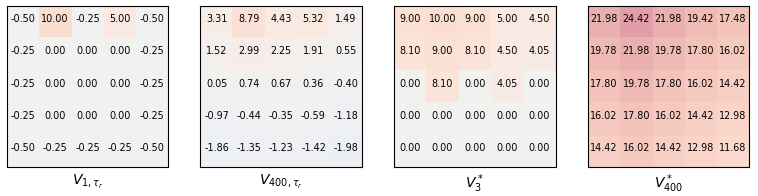
\includegraphics[scale=0.8]{figs/gridworld1.png}
    \caption{Value functions of the gridworld environment.
      Note that $V_{\max} \cdot \gamma^{400} = 100 \cdot (0.9)^{400}
      \approx 4.97 \cdot 10^{-17}$ so $V^*_{400}$ and $V_{\tau_r, 400}$
      are very close to the true infinite horizon value functions
    $V^*$ and $V_{\tau_r}$ (providing numerical errors are insignificant).}
    \label{fig:gw1}
  \end{figure}

  \begin{figure}[H]
    \centering
    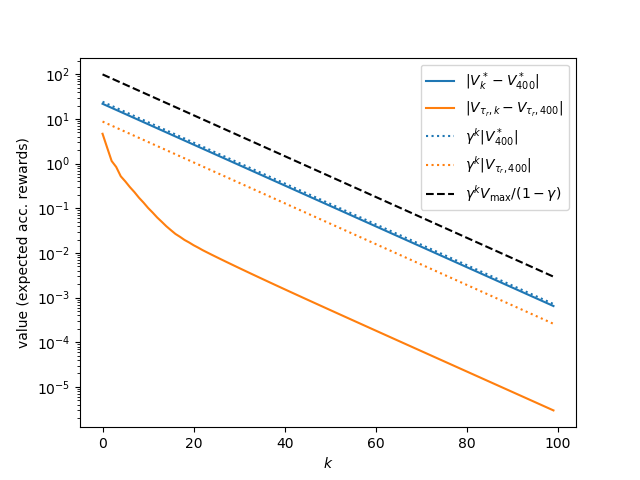
\includegraphics[scale=0.7]{figs/gridworld2.png}
    \caption{Convergence of gridworld value functions compared with
      the theoretical bounds. The black dashed line is the general theoretical
      bound for both $T$ and $T_{\tau}$ by Banachs fixed point theorem and
      the maximum value $V_{\max} = R_{\max} / (1-\gamma)$.
      The dotted blue and orange uses $\abs{V_k^*}$ and $\abs{V_{\tau, k}}$ 
      respectively, which might not be available.
    ($\gamma = 0.9$).}
    \label{fig:gw2}
  \end{figure}

  \label{ex:gridworld}
\end{example}

\subsection{Q-functions}

A \defemph{Q-function} is any function that assigns a real number
to every state-action pair, that is any function $Q : \cl{S} \times \cl{A}
\to \R$. Q-functions are also called \emph{action-value} functions,
to distinguish them from the \emph{value} functions we have discussed in the
previous sections.
The idea of Q-functions (and the letter Q) originates to
\mcite{W89}. Upon the definition he notes
\begin{displayquote}
  ``This is much simpler to calculate than [$V_\pi$]
  for to calculate [the greedy policy for $Q_\pi$] it is only necessary to look one
  step ahead [\ldots]''
\end{displayquote}
A clear advantage of working with Q-function
$Q:\Cal{S}\times\Cal{A} \to \R$ rather than a value function
$V:\Cal{S}\to \R$,
is that finding the optimal action $a^* \in \frak{A}(s)$ at state $s$
requires only a maximization over the Q-function itself:
$a^* = \argmax_{a \in \frak{A}(s)} Q(s,a)$.
This should be compared to finding an optimal action
according to a value function $V$:
$a^* = \argmax_{a \in \frak{A}(s)} r(s,a) + \gamma \E_{P(\cdot \mid s,a)} V$.
Besides being less simple,
this requires taking an expectation with respect to 
both the reward and transition kernel.
Later we will study settings where we can only sample from $P$ and $R$
when attempting to find the optimal strategy.
In these situations the advantage of Q-functions is clear.
For now however the transition kernel will remain known and we
will in this section see how the results of state-value functions
translate to Q-functions.
Because of the similar role Q-functions play compared to value function,
many concepts such as $T$-operators and the finite, infinite horizon
policy evaluations and greedy policies, can be defined analogously.

\begin{asm}[Finite admissable actions]
  $\frak{A}(s)$ is finite for every $s \in \cl{S}$. 
  \label{asm:finAdmAct}
\end{asm}
Throughout this section we will work under
\cref{sett:BS0} and \cref{asm:finAdmAct}.

\begin{rem}
  We make \cref{asm:finAdmAct} to ensure that the supremum
  $\sup_{a \in \frak{A}(s)} Q(s, a)$ is attained for any
  $Q \in \cl{L}_\infty(\cl{S} \times \cl{A})$.
  One might be able discard \cref{asm:finAdmAct} and instead
  demand that all Q-functions be
  upper semicontinuous generalizing the discussion in this section.
  We have not pursued this generalization.
\end{rem}

\begin{defn}[Policy evaluation for Q-functions]
  Let $\pi \in R\Pi$.
  Define
  \[ Q_{k, \pi}(s, a) = r(s, a) + \gamma \E_{P(\cdot \mid s, a)} V_{k, \pi}
  ,\qquad Q_\pi(s, a) = r(s, a) + \gamma \E_{P(\cdot \mid s, a)} V_\pi \]
  \[ Q^*_k = \sup_{\pi \in R\Pi} Q_{k, \pi}
  , \qquad Q^* = \sup_{\pi \in R\Pi} Q_\pi \]
  Define $Q_0 = r$ then we make the convention that
  $Q^*_0 = Q_{0,\pi} = Q_0 = r$.
  \label{defn:polEvalQ}
\end{defn}

\begin{defn}[Operators for Q-functions]
  For any stationary policy $\tau \in S\Pi$ and
  integrable Q-function $Q:\Cal{S} \times \Cal{A} \to \R
  \in \cl{L}_\infty(\cl{S} \times \cl{A})$ we define
  \begin{align*}
    \text{Next-step operator: }
    P_\tau Q(s, a) &= \int Q(s', a') \difd \tau P(s', a' \mid s, a)
    \\ \text{Policy evaluation operator: }
    T_\tau Q(s, a) &= 
    r(s, a) + \gamma \int Q(s', a') \difd \tau P(s', a' \mid s, a)
    \\ \text{Bellman optimality operator: }
      T Q(s, a) &= r(s, a) + \gamma
    \int \max_{a' \in \Cal{A}} Q(s', a') \difd P(s' \mid s, a)
  \end{align*}
  where $T_a = T_{\delta_a}$.
  \label{defn:opQ}
\end{defn}
\begin{rem}
  The next-step operator $P_\tau$
  is defined for simplications in proofs, especially
  in the analysis of \mcite{F20} in the later sections.
  Using $P_\tau$ we can write $T_\tau$ alternatively as
  $T_\tau Q(s, a) = r(s, a) + \gamma P_\tau Q (s, a)$.
\end{rem}
\begin{defn}[Greedy policies for Q-functions]
  Let $\tau : \Cal{S} \leadsto \Cal{A}$ be a stationary policy. Define
  $G_Q(s) = \argmax_{a \in \frak{A}(s)} Q(s, a)$.
  If there exist a measurable set $G_Q^\tau(s) \subseteq G_Q(s)$
  for every $s \in \Cal{S}$ such that
  \[ \tau \left( G_Q^\tau(s) \Mid s \right) = 1 \]
  then $\tau$ is said to be \defemph{greedy} with respect to $Q$ and is
  denoted $\tau_Q$.
  \label{defn:greedyQ}
\end{defn}

\begin{prop}[Relations between Q- and value functions]
  Let $\pi = (\tau_1, \tau_2, \dots) \in M\Pi$ be a Markov policy
  and $\tau \in S\Pi$ stationary. Then
  \leavevmode
  \begin{enumerate}
    \item Policy evaluations are related by
      $\E_{\tau(\cdot \mid s)} Q_{k, \pi} = V_{k+1, (\tau, \pi)}(s)$.
    \item $T_\tau$-operators are related by $T_\tau Q_{k, \pi}(s, a)
      = r + \gamma \E_{P(\cdot \mid s, a)} T_\tau V_{k, \pi}$.
    \item Greedy policies for policy evaluations are the same.
      That is
      \begin{enumerate}
	\item $\tau$ is greedy for
	  $Q_{k, \pi}$ if and only if $\tau$ is greedy for $V_{k, \pi}$.
	\item $\tau$ is greedy for $Q_\pi$ if and only if $\tau$ is greedy for
	  $V_\pi$.
      \end{enumerate}
    \item Optimal policies are related by
      $\max_{a \in \frak{A}(s)} Q^*(s, a) = V^*(s)$ and
      \[ Q^*_k(s, a) = r(s, a) + \gamma \E_{P(\cdot \mid s, a)} V^*_k,
      \quad Q^*(s, a) = r(s, a) + \gamma \E_{P(\cdot \mid s, a)} V^* \]
    \end{enumerate}
  \label{prop:relQV}
\end{prop}

\begin{prop}[Properties of Q-functions]
  Let $\pi = (\tau_1, \tau_2, \dots) \in M\Pi$ be a Markov policy
  and $\tau \in S\Pi$ stationary. Then
  \leavevmode
  \begin{enumerate}
    \item $Q_{k, \pi} = T_{\tau_1} \dots T_{\tau_k} Q_0$ and
      $Q^*_k = T_{\tau_{k-1}^*} \dots T_{\tau_0^*} Q^*_0
      = T^k Q^*_0$.
    \item $Q_\pi = \lim_{k \to \infty} Q_{k, \pi}$ and
      $Q^* = \lim_{k\to\infty} Q_k^*$. 
    \item $T,\; T_\tau$ are $\gamma$-contractive on
      $\Cal{L}_\infty(\Cal{S}\times\Cal{A})$
      and $Q^*,\; Q_\tau$ are their unique fixed points.
    \item $Q^* = Q_{\tau^*}$ and
      $Q_{k, \pi},\; Q_\pi,\; Q^*_k,\; Q^*$ are all upper semicontinuous
      and bounded by $V_{\max}$.
  \end{enumerate}
  \label{prop:propQ}
\end{prop}

\begin{proof}[Proof of \cref{prop:relQV} and \cref{prop:propQ}]
%todo fix this proof
  Measurability of $Q_{k, \pi}$ and $Q_\pi$
  follow from measurability of $V_{k, \pi}$, $V_{\pi}$
  and \cref{prop:intKerMeas}.
  Upper semicontinuity of $Q_{k, \pi}$ and $Q_\pi$ follows
  from \cref{prop:intSemiC} because $V_{k, \pi}$ and $V_\pi$ are
  upper semicontinuous (see \cref{cor:Viteration}).

  For \cref{prop:relQV}.1 we have \begin{align*}
    \E_{\tau(\cdot \mid s)} Q_{k, \pi}
    &= \int r(s,a) + \gamma \E_{P(\cdot \mid s, a)} V_{k, \pi}
    \difd \tau(a \mid s)
    \\ &= \int r(s,a) + \gamma \sum_{i=1}^{k} \gamma^{i-1} r(s_i, a_i)
    \difd P \tau_k \dots P\tau_1 P\tau(a, s_1, a_1, \dots, s_k \mid s)
  \\ &= V_{k+1, (\tau, \pi)} \end{align*}
  
  For \cref{prop:relQV}.2 we sketch the idea by
  \begin{align*}
    T_\tau Q_{k, \pi} = r + \gamma \int r + \gamma V_{k, \pi}
    \difd P \difd \tau P
    = r + \gamma \int r + \gamma V_{k, \pi} \difd P \tau \difd P
    = r + \gamma \int T_\tau V_{k, \pi} \difd P
  \end{align*}
  
  For $Q_{k,\pi} = T_{\tau_1} \dots T_{\tau_k} Q_0$ use \cref{prop:relQV}.2
  iteratively starting with
  $\tau = \tau_1, \pi = (\tau_2, \tau_3, \dots)$.
  
  The $\tau(Q_{k, \pi}) = \tau(V_{k, \pi})$ part of \cref{prop:relQV}.3
  is by definition of the two concepts of
  greedy functions.

  That $Q_\pi = \lim_{k \to \infty} Q_{k, \pi}$
  follows from dominated convergence and
  \cref{prop:VpiMeas}.3.

  For \cref{prop:relQV}.4 $Q_k^* = \sup_{\pi \in R\Pi} (r + \gamma \E V_{k,\pi})
  \leq r + \gamma \E V_k^* = r + \gamma \E V_{\pi_k^*}
  \leq Q_k^*$. The same argument works for the second part.

  Let $s \in \Cal{S}$ then $\sup_{a \in \frak{A}(s)} Q^*(s, a) = 
  \sup_{a \in \frak{A}(s)} (r(s, a) + \gamma \E_{P(\cdot \mid s, a)} V^*)
  = T V^*(s) = V^*(s)$.
  
  By the definition of $Q_{\tau^*}$ we have
  $Q^* = r + \gamma \E V^* = r + \gamma \E V_{\pi^*} = Q_{\tau^*}$.

  $T_\tau Q_\tau = T_\tau (r + \gamma \E \lim_{k\to\infty} T_\tau^k V_0)
  = \lim_{k\to\infty} T_\tau (r + \gamma \E T_\tau^k V_0)
  = \lim_{k\to\infty} (r + \gamma \E T_\tau^{k+1} V_0)
  = r + \gamma \E \lim_{k\to\infty} T^{k+1}_\tau V_0
  = r + \gamma \E V_\tau = Q_\tau$.

    We $T_{\tau_Q} Q = T Q$ for any measurable $Q$ because
  \[ T_{\tau_Q}(s, a) = r(s, a) + \gamma \int \max_{a' \in \frak{A}(s')} Q(s', a')
  \difd P(s' \mid s, a) = TQ(s, a) \]
  Therefore by \cref{prop:propQ}.1
  \[ T_{\tau_{k-1}^*} Q_{k-1, (\tau_{k-2}^*, \dots, \tau_0^*)}
  = T Q_{k-1}^* \]
  since by \cref{prop:relQV}.3 $\tau_{k-1}^*$ is greedy for $Q_{k-1}^*$.
  Now use induction to get $Q^*_{k-1} = T^k Q_0^*$.

  Because $V^* = V_{\tau^*}$ we have
  \[ TQ^* = T_{\tau^*} = r + \gamma \E T_{\tau^*} V_{\tau^*}
  = r + \gamma \E V^* = Q^* \]

  The contrativeness of $T$ and $T_\pi$ follows from the same argument as for
  value functions.
  Banach fixed point theorem now concludes \cref{prop:propQ}.3.

  Since now $Q^*$ and $Q_{\tau^*}$ are fixed points for $T$ they must be
  equal, concluding the last point, namely \cref{prop:propQ}.4.
\end{proof}

\subsubsection{Q-iteration}

Similar to the value iteration algorithm (\cref{alg:valueIteration}) we can
define the corresponding for Q-iteration.

\begin{figure}[H]
\begin{algorithm}[H] %\label{algocf:fq} % this labels line, could not fix
\caption{Simple theoretical Q-iteration}
\KwIn{MDP $(\Cal{S}, \Cal{A}, P, R, \gamma)$, number of iterations $K$}
Initialize the expected reward function:
$r \leftarrow \int x \difd R(x \mid \cdot)$.

Initialize the starting Q-estimator: $\wt{Q}_0 \leftarrow r$.

\For{$k = 0,1,2,\dots,K-1$}{
  Update the Q-estimator $ \wt{Q}_{k+1} = T \wt{Q}_k $
}
\KwOut{The $K$-optimal Q-function $Q^*_K = \wt{Q}_K$.}
\label{alg:theoSimpleQ}
\end{algorithm}
\end{figure}

By \cref{prop:propQ}.3 we thus have convergence of the \cref{alg:theoSimpleQ}:
\begin{cor}
  $\abs{Q^*_k - Q^*} \leq \gamma^k \norm{Q^*}_\infty
  \leq \gamma^k V_{\max}$.
  \label{prop:theoSimpleQConv}
\end{cor}

\subsection{Why are we not done?}

So far we have shown that value iteration under \cref{sett:BS0}
and Q-iteration under additionally \cref{asm:finAdmAct}, can solve
all such discounted MDPs with exponential convergence in $\gamma$.
This is a broad class of problems!
We name a few examples:
\begin{enumerate}
  \item Gridworld (\cref{ex:gridworld}).
  \item Board games like \emph{chess} and \emph{go}
    against a fixed (possibly randomized) opponent policy
    can be modelled accurately
    as such finite MDPs (putting $\gamma$ close to 1, so that winning late in 
    the game is still considered worth the effort).
  \item \emph{Pole balancing} in a 2D physical simulation environment
    (see e.g. the famous \emph{cartpole} example from \mcite{BSA83}).
    One may even add random effects (such as \emph{wind} effects)
    to make full use of our stochastic setup.
\end{enumerate}
The problem is of course that the value functions and operators
which are used in \cref{alg:theoSimpleQ} are not computable in practice.
For example the state space of chess is very large
(roughly $\abs{\cl{S}_{\hrm{chess}}} \geq 10^{43}$).
This means that if we were to use \cref{alg:theoSimpleQ} naively
(with finite implementation as \cref{ex:gridworld})
then we would have to store a vector of
roughly $N \cdot 10^{43}$ real numbers for each Q-function we define,
where $N$ is the average number of admissable actions at each state
$\frak{A}(s), s \in \cl{S}$
which has been estimated to around $35$ for chess.
This requires roughly $1.4 \cdot 10^{45}$ bytes, if each number is stored as a
single precision floating point number (4 bytes).
For comparison the entire digital data capacity in the world is estimated
less than $10^{23}$ bytes as of 2020.
Needless to say this is beyond any practical relevance.

The rest of this paper is therefore about the situations where we have
to use approximations and estimations for some or all of $P$, $R$ and
the Q-functions.

\section{Q-learning with function approximators}
In this section we will look at what happens if we
instead use approximations of the Q-functions and $T$ operator.
This means that we are in a setting where we can somehow
calculate $r$ and $TQ$ for any $(s,a) \in \cl{S} \times \cl{A}$,
but it is hard or infeasible to represent them (or at least one of them)
directly.
The purpose of this is to show how results about the convergence of Q-learning
is rather easily obtained if one has direct access
to the transition and reward kernels $P$ and $R$.

It seems to this author,
that this setting is not very well-studied in the case of a
continuous state space.
This is perhaps because it is considered solved
by the results of theoretical Q-learning presented in the previous section.
However as we have argued, this only have practical relevance 
when it is feasible to represent $TQ$.
Therefore we find it relevant to consider this setting in more detail.

What \emph{is} very well-studied is a further generalized setting
where $T$ and $r$ are assumed to be unknown,
that is, one has only access to their distributions via sampling from them.
Solutions for that setting are called \emph{model-free}.
We will deal with that setting in the next section.

\subsection{Algorithmic and approximation errors}

In the following we present some rather simple bounding techniques
which is inspired by arguments found in e.g. \ncite{F20},
together with some standard results from approximation theory
on artificial neural networks and Bernstein polynomials.

Let us consider any norm $\norm{\cdot}$ on
the set of Q-functions $\cl{Q} = \{ f: \cl{S} \times \cl{A} \to \R \}$.
Let $\cl{F} \subseteq \cl{Q}$ be some subclass of Q-functions
Let $\wt{Q}_0 \in \cl{F}$ be bounded in $\norm{\cdot}$.
Suppose we can approximate $T\wt{Q}_0$ by some $\wt{Q}_1 \in \cl{F}$
to $\ve_1 > 0$ precision and then approximate $T\wt{Q}_1$ by $\wt{Q}_2 \in \cl{F}$
and so on. This way we get a sequence of Q-functions satisfying
\begin{equation}
\norm{T\wt{Q}_{k-1} - \wt{Q}_k} \leq \ve_k, \forall k \in \N
\label{eq:defnvei}
\end{equation}

First observe that
\begin{align*}
  \norm{T^k \wt{Q}_0 - \wt{Q}_k}
  &\leq \norm{T^k \wt{Q}_0 - T \wt{Q}_{k-1}} + \norm{T\wt{Q}_{k-1} - \wt{Q}_k}
  \\ &\leq \gamma \norm{T^{k-1} \wt{Q}_0 - \wt{Q}_{k-1}}
  + \norm{T\wt{Q}_{k-1} - \wt{Q}_k}
\end{align*}

Using this iteratively we get
\begin{equation}
  \norm{T^k \wt{Q}_0 - \wt{Q}_k} \leq \sum_{i=1}^k \gamma^{k-i} \ve_i
  \label{eq:mbitb}
\end{equation}
This is sometimes called the \defemph{approximation error}
and we denote it
\begin{equation}
  \ve_{\mathrm{approx}}(k) \defeq \sum_{i=1}^k \gamma^{k-i} \ve_i
  \label{eq:defapproxe}
\end{equation}

Thus we get
\begin{thm}
  Let $\norm{\cdot}$ be a norm on the space of functions
  $\cl{S} \times \cl{A} \to \Rext$.
  Let $\wt{Q}_k$ be obtained from a function class $\cl{F}$
  such that $\norm{\wt{Q}_{k} - T\wt{Q}_{k-1}} \leq \ve_k$
  for any $k \in \N$. Then
  \[ \norm{Q^* - \wt{Q}_k} \leq \gamma^k \norm{Q^* - \wt{Q}_0}
  + \ve_{\mathrm{approx}}(k) \]
  \label{thm:genApprox}
\end{thm}
\begin{proof}
  By the discussion above and
  \begin{align*}
    \norm{Q^* - \wt{Q}_k}
    &\leq \norm{Q^* - T^k \wt{Q}_0} + \norm{T^k \wt{Q}_0 - \wt{Q}_k}
    \\ &
    \stackrel{\ref{eq:mbitb}}{\leq}
    \gamma^k \norm{Q^* - \wt{Q}_0} + \ve_{\mathrm{approx}}(k)
  \end{align*}
\end{proof}
The first term in \cref{thm:genApprox} is sometimes called the
\defemph{algorithmic} error\footnote{For example in \ncite{F20}.}.
The algorithmic error converges exponentially, so one is usually happy with this
part not spending time trying to bound this tighter.
The approximation error depends on our step-wise approximations. For example
if $\ve_i(k) = \ve$ for some $\ve > 0$ we easily get the bound
\begin{equation}
  \ve_{\mathrm{approx}}(k) = \ve \frac{1-\gamma^k}{1-\gamma} \leq \frac{\ve}{1-\gamma}
  \label{eq:approxEpsBound}
\end{equation}
If $\ve_i \leq c\gamma^i$ we get $\ve_{\mathrm{approx}}(k) \leq ck \gamma^k \to 0$ as
$k \to \infty$.
Generally if one can show that $\ve_i \to 0$ we have
\begin{prop} $ \sum_{i-1}^k \gamma^{k-i} \ve_i \to 0 $
  whenever $\ve_k \to 0$ as $k \to \infty$.
\end{prop}
\begin{proof}
  Let $\ve > 0$. Find $N$ such that $\ve_n \leq \ve (1-\gamma)/2$ 
  for all $n>N$ and find $M>N$ such that
  $\gamma^M \leq
  \ve \gamma^N \left( \sum_{i=1}^N \gamma^{N-i} \ve_i \right)^{-1}$.
  Then for all $m>M$
  \begin{align*}
    \sum_{i=1}^m \gamma^{m-i} \ve_i
    &\leq \gamma^{m-N} \sum_{i=1}^N \gamma^{N-i} \ve_i
    + \sum_{i=N+1}^m \gamma^{m-i} \ve (1-\gamma)/2
    \leq \ve/2 + \ve/2 \leq \ve
  \end{align*}
\end{proof}
We will now explore two different ways of obtaining bounds on the approximation 
error.

\subsection{Using artifical neural networks}

\begin{sett}[Continuous MDP]
  An MDP $(\cl{S}, \cl{A}, P, R, \gamma)$ with
  $\cl{S} = [0,1]^w$, $\cl{A}$ finite and
  a continuous expected reward function $r$.
  \label{sett:annApprox}
\end{sett}

\begin{defn}
  An \defemph{artificial neural network} (ANN) with $L \in \N_0$
  hidden layers, structure
  $(d_i)_{i=0}^{L+1} \subseteq \N$,
  activation functions $(\sigma_i)_{i=1}^L$,
  weights $(W_i)_{i=1}^{L+1} \in M^{d_i \times d_{i-1}}$ and
  biases $(v_i)_{i=1}^{L+1} \in \R^{d_i}$
  is the function $f:\R^{d_0} \to \R^{d_{L+1}}$ defined by
  \[ f = w_{L+1} \circ \sigma_L \circ w_L
  \circ \sigma_{L-1} \circ \dots \circ w_1 \]
  where $w_i$ is the affine function $x \mapsto W_i x + v_i$,
  and $\sigma_i : \R^{d_i} \to \R^{d_i}$ is coordinate-wise
  application of components $\sigma_{ij} : \R \to \R$.
  We denote the class of these networks (or functions)
  \[ \cl{DN} \left( (\sigma_i)_{i=1}^L,\; (d_i)_{i=0}^{L+1} \right) \]
  An ANN is called \emph{deep} if there are two or more hidden layers.
  \label{defn:ann}
\end{defn}

We shall often consider networks with only one type of activation functions,
i.e. all activation functions are equal to one function $\sigma: \R \to \R$.
We then write $f \in \cl{DN}\left(\sigma, (d_i)_{i=0}^{L+1} \right)$ as a
shorthand.

\begin{figure}[h]
  \centering
  \tikzset{%
    every neuron/.style={
      circle,
      draw,
      minimum size=0.5cm
    },
    neuron missing/.style={
      draw=none, 
      scale=2,
      text height=0.2cm,
      execute at begin node=\color{black}$\vdots$
    },
  }
  \begin{tikzpicture}[x=1cm, y=1cm, >=stealth]

    \foreach \m/\l [count=\y] in {1,2,3,missing,4}
    \node [every neuron/.try, neuron \m/.try] (input-\m) at (0,2.5-\y) {};

    \foreach \m [count=\y] in {1,missing,2}
    \node [every neuron/.try, neuron \m/.try ] (hidden-\m) at (2,2-\y*1.25) {};

    \foreach \m [count=\y] in {1,missing,2}
    \node [every neuron/.try, neuron \m/.try ] (output-\m) at (4,1.5-\y) {};

    \foreach \l [count=\i] in {1,2,3,d_0}
    \draw [<-] (input-\i) -- ++(-1,0)
    node [above, midway] {$x_{\l}$};

    \foreach \l [count=\i] in {1,d_1}
    \node [above=0.2cm] at (hidden-\i.north) { $n_{1, \l}$};

    \foreach \l [count=\i] in {1,d_2}
    \draw [->] (output-\i) -- ++(1,0)
    node [above, midway] {$f(x)_{\l}$};

    \foreach \i in {1,2,4} % 3 is looked at individually
    \foreach \j in {1,2}
    \draw [->] (input-\i) -- (hidden-\j);
      % 3
    \draw [->] (input-3) -- (hidden-2);

    \foreach \i in {1,...,2}
    \foreach \j in {1,...,2}
    \draw [->] (hidden-\i) -- (output-\j);

    \foreach \l [count=\x from 0] in {Input, Hidden, Ouput}
    \node [align=center, above, font=\footnotesize] at (\x*2,2)
    {\l \\ layer with \\ $d_{\x}$ nodes};
  \end{tikzpicture}
  \caption{An ANN with one hidden layer ($L=1$). Notice that there is no edge
    from $n_{0,3}$ to $n_{1,1}$ which means that
  $W_1(1,3) = 0$.}
\end{figure}

\begin{rem}
  Artificial neural networks are often illustrated as
  $L + 1$-partite graphs with $d_i$ nodes in the $i$th partition.
  A node $n_{i,j}$ in partition $i$ is then connected to a node
  $n_{i+1,k}$ if $W_{i+1}(k, j) \neq 0$.
  This is because they were
  inspired by the structure of \emph{neurons}
  in nerve tissue (e.g. the brain) of living organisms,
  with the graph nodes corresponding to neurons and edges to \emph{axons}.
  Indeed for every suitable collection of activation functions
  and every $L+1$-partite weighted graph $G$ satisfying
  \begin{equation}
    \text{\parbox{0.8\textwidth}{The $i$th partition is only
	connected to the neighboring $(i-1)$th and $(i+1)$th partition.
    }}
    \label{eq:graphANN}
  \end{equation}
  Then there exists a corresponding ANN corresponding to $G$.
  From the graph view-point it easy to see that one may join neural nets
  to form larger ones, by either function composition or side-by-side
  alignment.
  That this if
  $f \in \cl{DN}\left( (\sigma_i)_{i=1}^{L},\; (d_i)_{i=0}^{L + 1} \right)$
  and
  $g \in \cl{DN}\left( (\sigma'_i)_{i=1}^{L'},\; (d'_i)_{i=0}^{L' + 1} \right)$
  are two ANNs and $d_{L+1} = d_0'$ (i.e. that
  the dimensions match $\hrm{im}(f) \subseteq \hrm{dom}(g)$)
  then
  $g \circ f \in \cl{DN}
  \left( (\sigma_1, \dots, \sigma_L, \sigma'_1, \dots,
  \sigma'_{L'}), (d_1, \dots, d_L, d'_1, \dots, d'_{L'}) \right)$.
  By side-by-side alignment we mean the situation where $L = L'$
  and one creates the function
  $h : \R^{d_0 + d'_0} \to \R^{d_L + d'_L}$
  by defining $h(x_1, \dots, x_{d_0 + d'_0})
  = (f(x_1, \dots, x_{d_0}), g(x_1, \dots, x_{d'_0}))$.
  With this way of defining $h$ we have that
  $h$ is an ANN with structure $(d_0 + d'_0, \dots, d_{L+1} + d'_{L+1})$.
  Generally any way of stitching together graphs into $n$-partite graphs
  satisfying \cref{eq:graphANN}
  will gives ways of producing new ANNs. 
  \label{rem:annGraph}
\end{rem}

\begin{thm}[Universal Approximation Theorem for ANNs]
  Let $\sigma: \R \to \R$ be non-constant, bounded and continuous
  activation function.
  Let $\ve > 0$ and $f \in C([0,1]^w)$.
  Then there exists an $N \in \N$ and a network
  $F \in \cl{DN}(\sigma, (w, N, 1))$
  with one hidden layer,
  unbiased final layer (that is $v_2 = 0$)
  and activation function $\sigma$ such that
  \[ \norm{F - f}_\infty < \ve \]
  In other words $\bigcup_{N \in \N} \cl{DN}(\sigma, (w, N, 1))$ is
  dense in $C([0,1]^w)$.
  \label{thm:uniApprox}
\end{thm}
\begin{proof}[Discussion of proofs of \cref{thm:uniApprox}]
  The original proof in \mcite{C89} is very short and elegant,
  but non-constructive,
  using the Riesz Representation and Hahn-Banach theorems to
  obtain a contractiction to the statement that
  $\bigcup_{N \in \N} \cl{DN}(\sigma, (w,N,1))$
  is dense in $C([0,1]^w)$.
  Furthermore it considered only \emph{sigmoidal} activations
  functions, meaning that $\sigma$ should satisfy
  \[ \sigma(x) \to \begin{cases} 0 & x \to -\infty
  \\ 1 & x \to \infty \end{cases} \]
  
  This was extended in \mcite{CCR90} to the statement as presented above
  and their proof is constructive. 
\end{proof}

We will now show how ANNs can be used to approximate the optimal
value function to arbitrary precision,
and look at a particular class of ANNs called \emph{ReLU networks},
which are defined by their use of the \emph{ReLU activation function}
$\sigma_r(x) = \max(0, x)$.

\begin{defn}
  We define the class of ReLU networks as the ANNs (see \cref{defn:ann})
  with all ReLU activation functions, and write
  $\cl{RN}\left( (d_i)_{i=0}^{L+1} \right)
  \defeq \cl{DN}\left( \sigma_r, (d_i)_{i=0}^{L+1} \right)$. 
  \label{defn:relu}
\end{defn}

\begin{prop}
  Under \cref{sett:annApprox} let $\varepsilon > 0$.
  Assume that either
  \begin{enumerate}
    \item $P$ is deterministic with $P(\cdot \mid s, a) = \delta_{p(s, a)}$.
      For some continuous $p: \cl{S} \times \cl{A} \to \cl{S}$.
  \end{enumerate}

  or
  \begin{enumerate}[resume]
    \item $P(\cdot \mid s, a)$ is absolutely continuous
      with respect to the same measure $\nu$ on $\cl{S}$ for all
      $(s, a) \in \cl{S} \times \cl{A}$ with density
      $p(\cdot \mid s, a)$ which is continuous in $s$.
  \end{enumerate}
  Then for every $k \in \N$ there exists a $N\in \N$ and a sequence of
  Q-networks $(\wt{Q}_i)_{i=1}^k \subseteq \cl{RN}(w \abs{\cl{A}}, N, 1)$
  such that
  \[ \ve_{\mathrm{approx}}(i) = \norm{T\wt{Q}_{i-1} - \wt{Q}_i}_\infty < \ve \]
  for all $i \in [k]$.
  In particular
  \[ \abs{Q^* - \wt{Q}_k} < \varepsilon/(1 - \gamma) \]
\end{prop}
\begin{proof}[Proof]
  The key points are that
  \begin{enumerate}[label=\alph*.]
    \item Any ANN with continuous activation functions is continuous.
    \item Under assumptions 1. or 2. the Bellman operator $T$ preserves
      continuity.
    \item It is possible to join a finite number of ReLU networks
      $f_{a_1}, \dots, f_{a_\frak{a}} : \cl{S} \to \R$
      into a bigger ReLU network $f : \cl{S} \times \cl{A} \to \R$
      such that $f(s, a) = f_a(s)$.
  \end{enumerate}

  Using these facts we can use the universal approximation theorem
  (\cref{thm:uniApprox}) to get a series of networks
  \[ f_{a, k} : \cl{S} \to \R \]
  for each $a \in \cl{A}$ and $k \in \N$ satisfying
  \begin{equation}
    \abs{f_{a, k} - T \wt{Q}_{k-1}(\cdot, a)} < \ve
    \label{eq:ann_approx_1}
  \end{equation}
  Here $\wt{Q}_0 = r$ and $\wt{Q}_k$ is obtained recursively by
  joining for each $a$ the components $f_{a, k}$ into a single network
  $\wt{Q}_k : \cl{S} \times \cl{A} \to \R$ such that
  $\wt{Q}_k(s, a) = f_{a, k}(s)$.
  By \cref{eq:ann_approx_1} on each of its components
  approximates $T \wt{Q}_{k-1}$ to $\ve$ precision.
  $\wt{Q}_0$ is continuous by \cref{sett:annApprox} and by
  a. and b. $T \wt{Q}_k$ is as well.
  
  We will now establish points a., b. and c.
  \begin{enumerate}[label = \alph*.]
  \item follows by the fact that that composition of continuous functions
    are continuous.
  \item Let $Q: \cl{S} \times \cl{A} \in \cl{L}_\infty(\cl{S} \times \cl{A})$
    be continuous and let
    $x_1, x_2, \dots \in \cl{S} \times \cl{A}$ with
    $x_\ell \to x \in \cl{S} \times \cl{A}$.
    We will show that
    under 1. or 2. we have $TQ(x_\ell) \to TQ(x)$.
    \begin{enumerate}[label = \arabic*.]
      \item In this case $TQ(x) = r(x) + \gamma
	\max_{a' \in \cl{A}} Q(p(x), a')$ can be seen as the composition
	of the continuous functions $p$, $Q$, $\max$, $+$ and $r$.
      \item We have by dominated convergence and the assumption that
	$r$ is continuous (see \cref{sett:annApprox}) that
	\begin{align*}
	  TQ(x_\ell) &= r(x_\ell) + \gamma \int \max_{a'\in \cl{A}}
	  Q(s', a') p(s' \mid x_\ell) \difd v(s')
	  \\ &\to r(x) + \gamma \int \max_{a'\in \cl{A}}
	  Q(s', a') p(s' \mid x) \difd v(s')
	  \\ &= TQ(x)
	\end{align*}
    \end{enumerate}
  \item Let $k \in \N$.
    To join the components $f_{a, k}$ into a single network
    we embed $\cl{A}$ into $[0,1]^\frak{a}$ (where $\abs{\cl{A}} = \frak{a}$)
    by enumerating the actions $\cl{A} = \{ a_1, a_2, \dots, a_\frak{a} \}$
    and putting $a_i = (0,\dots,0,1,0,\dots,0)$ where the 1 is on the $i$th
    spot (this is called the \emph{one-hot embedding}).
    Let $L_a, (d_{a, i})_{i=0}^{L_a + 1}$ denote the number of hidden layers 
    and structure of $f_{a, k}$.
    We can now define $\wt{Q}_k : [0,1]^{w + \frak{a}} \to \R$
    as the ReLU network with 
    $L = 2 + \max_{a \in \cl{A}} L_a$ hidden layers and structure
    $d_0 = w + \frak{a}$, $d_1 = w \cdot \frak{a}$ and
    $d_i = \sum_{a \in \cl{A}} d'_{a, i-1}$ for $i = 2, \dots L-1$ putting
    $d'_{a, i} = d_{a, i}$ for $1 \leq i \leq L_a - 1$
    and $d'_{a, i} = d_{a, L_a}$ for $L_a \leq i \leq L - 1$
    then $d_L = \frak{a}$
    and finally $d_{L + 1} = 1$.
    The first layer consist of the affine map
    $w_1 : \R^{w + \frak{a}} \to \R^{w \cdot \frak{a}}$ defined by
    \[ w_1(s, 0, \dots, 1, \dots, 0)
    = (s, \dots, s + 1, \dots, s) - 1 \]
    where $s = (s_1, \dots, s_w) \in \R^w$ and where
    we use the notation $1 = (1, \dots, 1) \in \R^k$ for any $k \in \N$.
    Applying the ReLU activation $\sigma_r = \max(0, \cdot)$
    coordinate-wise we get
    \[ \sigma_r(w_1(s, 0, \dots, 1, \dots, 0)) =
    (0, \dots, s, \dots, 0) \]
    since all $s_i \in [0,1]$, so $\max(0, s_i - 1) = 0$ and
    $\max(0, s_i) = s_i$.
    We now use the component networks middle part of the network of $\wt{Q}_k$.
    For $2 \leq i \leq L$ put
    $w_i = (w_{1, i-1}, \dots, w_{\frak{a}, i-1}) : \R^{d_{i-1}} \to \R^{d_i}$ 
    where we define
    \[ w_{j, i} = \begin{cases}
	\text{the $i$th affine map of } f_{a_j, k} & 1 \leq i \leq L_{a_j}
	\\ \text{the identity map: } 
	\id : \R^{d_{a_j, i-1}} \to \R^{d_{a_j, i}} & L_{a_j} < i < L
	\\ \text{the $i$th affine map of } f_{a_j, L_{a_j} + 1} & i = L
	\\ \text{summation: } (x_1, \dots, x_\frak{a}) \mapsto
	\sum_{\ell = 1}^\frak{a} x_\ell & i = L + 1
    \end{cases} \]
    With this construction we have that
    $\wt{Q}_k(s, a) = f_{a, k}(s)$
    for all $a \in \cl{A}$.
    And that $\wt{Q}_k(s, a) \in \cl{RN}(w + \frak{a}, w\cdot \frak{a}
    , d_2, \dots, d_{L-1}, d_\frak{a}, 1)$.
\end{enumerate}
\end{proof}

This gives us the first method of how to approximate
$Q^*$ arbitrarily closely on continuous state spaces, in the case
where it is infeasible to represent $TQ$ directly.
However it is still not clear if this method is feasible
computationally.
To investigate this and indeed for any chance to implement the method
in practice one would need to go through the
construction in \ncite{CCR90}. We will not go further into this,
and instead focus on another approximation method using
\emph{Bernstein polynomials}.

\subsection{Using Bernstein polynomials}

In this case we need a stronger form of continuity, namely
Lipschitz continuity (see \cref{defn:Lipschitz}), to establish the bounds.

\begin{sett}[Bernstein approximable MDP]
  An MDP $(\cl{S}, \cl{A}, P, R, \gamma)$ with
  $\cl{S} = [0,1]^w$ and $\cl{A}$ finite.
  Assume that there exists a probability measure $\mu \in \cl{S}$, such that
  $P(\cdot \mid s, a)$ has density
  $p(\cdot \mid s, a) : \cl{S} \to \R$ with respect to
  $\mu$ for all $(s, a) \in \cl{S}\times\cl{A}$. 
  Furthermore assume that $r(\cdot, a), \; p(s \mid \cdot, a)$ are
  $\norm{\cdot}$-Lipschitz
  with constants $L_r,\; L_p$ respectively for all
  $(s, a) \in \cl{S} \times \cl{A}$
  for some norm $\norm{\cdot}$.
  \label{sett:polyApprox}
\end{sett}

\begin{defn}[Bernstein polynomial]
  The (multivariate) Bernstein polynomial $B_{f, n}$ of degree
  $n=(n_1, \dots, n_w) \in \N^w$ approximating the function $f:[0,1]^w \to \R$
  is defined by
  \begin{equation*}
    B_{f, n}(x_1, \dots, x_w) =
    \sum_{j = 1}^w \sum_{k_j = 0}^{n_j}
    f\left( \frac{k_1}{n_1}, \dots, \frac{k_w}{n_w} \right)
    \prod_{\ell = 1}^w \left(
    \binom{n_\ell}{k_\ell} x_\ell^{k_\ell}(1-x_\ell)^{n_\ell - k_\ell} \right)
  \end{equation*}
  \label{defn:Bfn}
\end{defn}
Notice that this a polynomial of (multivariate) degree
$\norm{n}_1 = n_1 + \dots + n_w$.

\begin{thm}[Approximation with Bernstein polynomials]
  Let $f : [0,1]^w \to \R$ be Lipschitz
  w.r.t. the standard euclidean 2-norm induced metrics on $[0,1]^w$ and $\R$
  with constant $L$. 
  Let $n = (n_1, \dots, n_w) \in \N^w$.
  The Bernstein polynomial
  $B_{f,n} : [0,1]^w \to \R$ satisfies
  \begin{enumerate}
    \item $\norm{f - B_{f,n}}_\infty
      \leq \frac{L}{2} \sqrt{\sum_{j=1}^w \frac{1}{n_j}}$
    \item $\norm{B_{f,n}}_\infty \leq \norm{f}_\infty$
  \end{enumerate}
  \label{thm:bernsteinApprox}
\end{thm}
\begin{proof}
  We refer to \mcite{H02} thm. B..7.
\end{proof}

\begin{lem}
  Under \cref{sett:polyApprox} 
  $TQ(\cdot, a)$ is Lipschitz in $\norm{\cdot}_2$ with constant
  $ L_T = L_r + \gamma V_{\max} L_p $
  for all $a \in \cl{A}$ and measurable
  $Q : \cl{S} \times \cl{A} \to [-V_{\max},V_{\max}]$.
  \label{lem:bernsteinLem}
\end{lem}
\begin{proof}
  Because of the Lipschitz property of $r$ and $p$ we have
  for any measurable $Q : \cl{S} \times \cl{A} \to [-V_{\max},V_{\max}]$
  and $s \neq s' \in \cl{S}$ that
  \begin{align*}
    \abs{TQ(s, a) - TQ(s', a)}
    &\leq \abs{r(s, a) - r(s', a)} 
    \\ &+ \gamma \int
    \abs{\max_{a'\in\cl{A}}Q(s'', a') p(s'' \mid s, a)
    - \max_{a'' \in \cl{A}} Q(s', a'') p(s'' \mid s', a) }
    \difd \mu(s'')
    \\ &\leq L_r \norm{s - s'} + \gamma \int
    \abs{\max_{a'\in\cl{A}}Q(s', a')}
    \abs{p(s'' \mid s, a) - p(s'' \mid s', a)}
    \difd \mu(s'')
    \\ &\leq L_r \norm{s - s'} + \gamma \int
    V_{\max}
    L_p \norm{s - s'}
    \difd \mu(s'')
    \\ & = (L_r + \gamma V_{\max} L_p) \norm{s - s'}
  \end{align*}
\end{proof}

Using this we can make a bound on the approximation error:

\begin{prop}
  Given an MDP satisfying \cref{sett:polyApprox} and using $\norm{\cdot}_\infty$
  we can bound
  \[ \ve_{\mathrm{approx}} \leq \frac{L_r + \gamma V_{\max} L_p}{2(1-\gamma)}
  \sqrt{\sum_{j=1}^w \frac{1}{n_j}} \]
  \label{prop:veapproxlibbound}
\end{prop}
\begin{proof}
  Following the procedure from leading to \cref{eq:mbitb},
  starting with $\wt{Q}_0 = 0$
  and using the $n = (n_1, \dots, n_w)$ degree Bernstein polynomium
  $\wt{Q}_{k} = B_{T\wt{Q}_{k-1}, n}$ as approximation for $T\wt{Q}_{k-1}$
  we know by induction and
  the results \cref{lem:bernsteinLem}
  and \cref{thm:bernsteinApprox}.2 that $T\wt{Q}_k$ is
  $L_T$-Lipschitz for any $k \in \N$.
  Now by choosing the euclidean norm $\norm{\cdot} = \norm{\cdot}_2$
  we have by \cref{thm:bernsteinApprox}.1 that
  \begin{equation}
    \ve_i = \norm{\wt{Q}_k - T\wt{Q}_{k-1}}_\infty
    \leq \frac{L_T}{2} \sqrt{\sum_{j=1}^w \frac{1}{n_j}} = \ve
    \label{eq:veapproxlib1}
  \end{equation}
  where $\ve$ is the one-step error defined in \cref{eq:defnvei}.
  Now by \cref{eq:approxEpsBound}
  we have that
  \begin{equation}
    \ve_{\hrm{approx}} \leq \frac{\ve}{1-\gamma}
    \label{eq:veapproxlib2}
  \end{equation}
  Combining \cref{eq:veapproxlib1} and \cref{eq:veapproxlib2} and noting
  that $L_T = L_r + \gamma V_{\max} L_p$ finishes the proof.
\end{proof}

To make more clear what are the implications of \cref{prop:veapproxlibbound}
we give a corollary where we put $n_j = m$ for all $j \in [w]$:

\begin{cor}
  Under \cref{sett:polyApprox} and using Bernstein polynomials of degree
  $n = (m, \dots, m) \in \N^w$ for $m \in \N$ we have the following bound
  \[ \norm{Q^* - \wt{Q}_k}_\infty \leq \gamma^{-k} V_{\max}
    + \frac{L_r + \gamma V_{\max} L_p}{2(1-\gamma)} \sqrt{w}
  \frac{1}{\sqrt{m}} \]
  In particular $\norm{Q^* - \wt{Q}_k}_\infty
  = \cl{O}(\gamma^{-k} + \frac{1}{\sqrt{m}})$
  when using $k$ iterations.
  \label{cor:libbound}
\end{cor}
\begin{proof}
  Use \cref{prop:veapproxlibbound}.
\end{proof}

This gives a very concrete way of constructing an arbitrarily good
approximation to $Q^*$ using polynomials.
A major drawback is the restriction on the transition dynamics $P$.
For example we cannot use \cref{cor:libbound} on deterministic
decision processes, since if $P$ is deterministic then there
are no measure $\mu \in \cl{P}(\cl{S})$ which allows for a
density $p(\cdot \mid s, a)$ (i.e. $p \cdot \mu = P(\cdot \mid s, a)$),
unless $P(\cdot \mid s, a) = \delta_{s'}$ for all $(s, a) \in \cl{S} \times
\cl{A}$, which would lead to a quite boring environment.
Generally the processes with fast convergence bounds 
according to \cref{cor:libbound} must be very stochastic.
%todo example.

This concludes our investigation of model-based Q-learning and we will
now look at the much more well-studied field of model-free Q-learning.



\chapter{Model-free algorithms}

In this section we will look at what can be done when the process dynamics
are unknown.
In this case we cannot calculate directly neither $r$, $T_\pi Q$ nor
$TQ$ because the transition and reward kernels $P,R$ are unknown.

It is clear that \cref{alg:theoSimpleQ} will not work without
modification in this case. Simply because $R$ and $P$ are not
available.
To make the scheme work anyway we could simply avoid taking expectations
and use the random outcomes of the kernels.
Leading to

\begin{figure}[H]
\begin{algorithm}[H] %\label{algocf:fq} % this labels line, could not fix
  \caption{Random theoretical Q-iteration (example of thought)}
\KwIn{MDP $(\cl{S}, \cl{A}, P, R, \gamma)$, number of iterations $K$}
$\forall (s, a) \in \cl{S} \times \cl{A} :
\wt{Q}_0(s, a) \leftarrow X \sim R(\cdot \mid s, a)$.

\For{$k = 0,1,2,\dots,K-1$}{
  $ \forall (s, a) \in \cl{S} \times \cl{A} :
  \wt{Q}_{k+1}(s, a) \leftarrow r'
  + \gamma \sup_{a' \in \cl{A}} \wt{Q}_k(s', a')$

  where $r' \sim R(\cdot \mid s, a), s' \sim P(\cdot \mid s, a)$.
}
Define $\pi_K$ as the greedy policy w.r.t. $\wt{Q}_K$ \\
\KwOut{An estimator $\widetilde{Q}_K$ of $Q^*$ and policy $\pi_K$}
\label{alg:theoRandomQ}
\end{algorithm}
\end{figure}
We immedially run into problems in the uncountable case, because
drawing uncountably many times from a distribution is not easily
defined in a sensible way.
Even in the finite case where the functions $\wt{Q}_k$
are well defined, they cannot converge if $R$ is not deterministic.
Therefore this approach does not work in a continuous or
stochastic setting.

There are broadly two ways of dealing with these
problems\footnote{This classification is discussed in \mcite{K99}.}.
In the \emph{indirect} approaches one tries to first estimate $P$ and $R$
by sampling.
We can then use the model-dependent methods of the last chapter using
estimated kernels $\wt{P}$ and $\wt{R}$.
We will not go further into indirect methods in this thesis.
The \emph{direct} approaches covers \emph{the rest},
and it is mainly these were are going to look at throughout this
paper. A popular indirect approach is called
\emph{temporal difference} (TD) learning and was initially invented 
for finite MDPs.

\section{Finite case}

\begin{sett}[Finite MDP]
  An MDP $(\cl{S}, \cl{A}, P, R, \gamma)$ where
  $\abs{\cl{S}} = \frak{s} \in \N$ and $\abs{\cl{A}} = \frak{a} \in \N$
  are finite.
\end{sett}

TD learning is based on the following
update scheme
\begin{equation}
  \wt{Q}_{k+1}(s, a) \leftarrow (1-\alpha_k) \wt{Q}_k(s, a)
  + \alpha_k (r' + \gamma \cdot \max_{a' \in \cl{A}} \wt{Q}_k(s', a'))
  \label{eq:tdeq}
\end{equation}
Here $r'$ and $s'$ are the reward and next-state drawn from the
reward and transition kernels,
and $\alpha_k \in [0,1]$ is the so-called \defemph{learning rate}
(of the $k$th step).
The 'temporal difference' is also the name of term
$ \alpha_k ( r' + \gamma \cdot \max_{a \in \cl{A}} \wt{Q}_k(s', a')
- \wt{Q}_k(s, a) )$ occuring from rearranging \cref{eq:tdeq}.
Usually the learning rate is fixed before running the algoritm
(does not depend on the history) and is set to decay
from 1 to 0 in some fashion as $k \to \infty$.

We will now look at a convergence result originally obtained in
\mcite{WD92} of a TD algorithm using Q-functions.
The result was extended slightly in \mcite{J94} and is here presented
more in the style of \ncite{J94}.
\begin{figure}[H]
\begin{algorithm}[H] %\label{algocf:fq} % this labels line, could not fix
  \caption{Finite asynchronos Q-learning}
  \KwIn{Finite MDP $(\cl{S}, \cl{A}, P, R, \gamma)$,
    i.e. $\abs{\cl{S}}\abs{\cl{A}} < \infty$,
    number of iterations $K$,
    state-action pairs $(s_1,a_1, \dots, s_K, a_K)$,
    learning rates $(\alpha_1', \dots, \alpha_K')$,
    initial $\wt{Q}_0 : \cl{S}\times\cl{A} \to \R$
  }
  Put $\alpha_k(s, a) \leftarrow \begin{cases}
    \alpha'_k & (s, a) = (s_k, a_k)
    \\ 0 & (s, a) \neq (s_k, a_k)
  \end{cases}$.

  \For{$k = 1,2,\dots,K$}{
    Sample $r' \sim R(\cdot \mid s_k, a_k),
    s' \sim P(\cdot \mid s_k, a_k)$

    Update action-value function:
    \[ \wt{Q}_k \leftarrow
      \wt{Q}_{k-1} +
      \alpha_k (r' + \max_{a' \in \cl{A}} \wt{Q}_{k-1}(s', a'))
    \]
  }
  Define $\pi_K$ as the greedy policy w.r.t. $\wt{Q}_K$ \\
  \KwOut{An estimator $\widetilde{Q}_K$ of $Q^*$ and policy $\pi_K$}
  \label{alg:finAsyncQL}
\end{algorithm}
\end{figure}
Note that only the value of the pair $(s_k, a_k)$ are updated in each
step of the algorithm
(since $\alpha_k(s, a) = 0$ for all $(s,a)\neq(s_k, a_k)$).

\begin{thm}[Watkins, Dayan 1992]
  Let $s_1, a_1, s_2, a_2, \dots \in
  \cl{S} \times \cl{A} \times \cl{S} \times \cl{A} \times \dots$
  be random variables, and $\alpha_1, \alpha_2, \dots \in [0,1]$.
  The output $\wt{Q}_K$ of \cref{alg:finAsyncQL} converges to $Q^*$
  provided
  \begin{enumerate}
    \item $\Prob\left(\sum_{i=1}^\infty \alpha_i(s,a) = \infty\right) = 1,
      \Prob\left(\sum_{i=1}^\infty \alpha_i^2(s,a) < \infty\right) = 1$.
    \item $\Var(R(\cdot \mid s, a)) < \infty$ for all $(s, a) \in
      \cl{S}\times\cl{A}$.
    \item If $\gamma = 1$ all policies lead to a reward-free terminal
      state almost surely.
  \end{enumerate}
\end{thm}
In the original formulation the sums of learning rates were supposed to
converge \emph{uniformly}. However this is equivalent to this formulation
because of the fact that
$\Prob(\sup_{(s, a) \in \cl{S} \times \cl{A}} \abs{f_n(s, a)} \to 0) = 1 \iff
\Prob\left(\;\abs{f_n(s, a)} \to 0 \right) = 1,
\forall (s, a) \in \cl{S} \times \cl{A}$
whenever $\cl{S}, \cl{A}$ is finite.
Notice that the first condition implies that all state-action pairs
occur infinitely often almost surely.
Also notice that the second condition is automatically fulfilled under
(D) since then $\Var(R(\cdot \mid s, a)) \leq \E (2R_{\max})^2 = 4 R_{\max}^2$.

%% Szepesvári Asymptotic convergence-rate of Q-learning 1997
In a special case of the same setup, convergence rates where
established by \mcite{S97}.
\begin{thm}[Szepesvári]
  Let $t \in \N$ and
  $s_1, a_1, s_2, \dots, s_t, a_t$ be sampled i.i.d. from
  $p \in \cl{P}(\cl{S} \times \cl{A})$.
  Set the learning rates such that
  $\alpha'_k
  = |\{ i \in [k-1] \mid (s_i, a_i) = (s_k, a_k) \}|^{-1}$,
  i.e. the reciprocal of the frequency of $(s_k, a_k)$ at step $k$.
  Let $\beta = \max_{x \in \cl{S} \times \cl{A}} p(x) /
  \min_{x \in \cl{S} \times \cl{A}} p(x)$.
  Then for some $B > 0$ the following holds asymptotically almost surely
  \begin{equation}
    \abs{\wt{Q}_t - Q^*} \leq B \frac{1}{t^{\beta (1-\gamma)}}
    \label{eq:Szepesvari1}
  \end{equation}
  and
  \begin{equation}
    \abs{\wt{Q}_t - Q^*} \leq B \sqrt{\frac{\log \log t}{t}}
    \label{eq:Szepesvari2}
  \end{equation}
\end{thm}
Here \cref{eq:Szepesvari1} is tightest when $\gamma > 1 - \beta/2$
otherwise \cref{eq:Szepesvari2} is tighter.
%todo find out if we wanna do proof

A paper \mcite{MH18} proves that $Q$-learning is PAC-learnable
given some additional assumptions.

\begin{algorithm}[H] %\label{algocf:fq} % this labels line, could not fix
  \caption{Finite synchronos Q-learning}
  \KwIn{MDP $(\cl{S}, \cl{A}, P, R, \gamma)$ such that
    $\abs{\cl{S}}\abs{\cl{A}} < \infty$,
    number of iterations $K$,
    learning rates $(\alpha_1, \dots, \alpha_K)$,
    initial $\wt{Q}_0 : \cl{S}\times\cl{A} \to \R$
  }

  \For{$k = 1,2,\dots,K$}{
    Sample $r' \sim R(\cdot \mid s_k, a_k),
    s' \sim P(\cdot \mid s_k, a_k)$

    Update action-value function:
    \[ \wt{Q}_k \leftarrow
      \wt{Q}_{k-1} +
      \alpha_k (r' + \max_{a' \in \cl{A}} \wt{Q}_{k-1}(s', a'))
    \]
  }
  Define $\pi_K$ as the greedy policy w.r.t. $\wt{Q}_K$ \\
  \KwOut{An estimator $\widetilde{Q}_K$ of $Q^*$ and policy $\pi_K$}
  \label{alg:finSyncQL}
\end{algorithm}


\begin{thm}[Mansour 2003]
  Assume (P) and (D). Let $\alpha_k = 1/(k+1)^\omega$ where
  $\omega \in (1/2,1]$.
  Fix $C>0$, a sufficiently large constant.
  Let $\ve, \delta >0$ and define
  \[ A = \frac{4V^2_{\max} \log(2\abs{\cl{S}}\abs{\cl{A}} V_{\max}/\delta
  (1-\gamma)\ve)}{(1-\gamma)^2\ve^2}, \quad B= 2 \log(V_{\max}/\ve)/(1-\gamma) \]
  The following hold for any $\psi > 0$.

  If the synchronos algorithm (\cref{alg:finSyncQL}) is run with
  \[ K \geq C \begin{cases}
      A^{1/\omega} + B^{1/(1-\omega)} & \omega \in (1/2,1)
      \\ \frac{(2 + \psi)^B}{\psi^2} \left(A +
      \frac{4 V^2_{\max} \log(1/\psi)}{(1-\gamma)^2 \ve^2} \right)
      & \omega = 1
    \end{cases}
  \]
  then with probability at least $1-\delta$ we have
  $\norm{\wt{Q}_K - Q^*}_\infty < \ve$.

  If the asynchronos algorithm (\cref{alg:finAsyncQL}) with 
  \[ K \geq C \begin{cases}
      (L^{1 + 3 \omega} A)^{1/\omega} + (L B)^{1/(1-\omega)}
      & \omega \in (1/2,1)
      \\ \frac{(L + \psi L + 1)^B}{\psi^2}
      \left(A + \frac{4V^2_{\max} \log(1/\psi)}{(1-\gamma)^2\ve^2} \right)
	& \omega = 1
  \end{cases} \]
  and the state-action pairs $(s_1, a_1, \dots, s_K, a_K)$ are drawn
  from a distribution such that every pair in $\cl{S}\times\cl{A}$
  appears in every sequence of length at least $L > 0$,
  then with probability at least $1-\delta$ we have
  $\norm{\wt{Q}_K - Q^*}_\infty < \ve$.
  \label{thm:mansour2003}
\end{thm}
In \ncite{MH18} $L$ is called the \emph{covering rate}.

\begin{rem}
An interesting side note to \cref{thm:mansour2003} is that
one can use the bounds to give hints at how to tune the learning rate
by changing $\omega$. Optimizing for different scenarios yield
different learning theoretically optimal values for $\omega$.
For example if we want to optimize for the bound on $K$ for 
$\gamma \to 1$ using the synchronos algorithm,
we get the following rate (treating other variables as constant)
$K \geq C'(1/(1-\gamma)^{4/\omega} + 1/(1-\gamma)^{1/(1-\omega)})$
for some $C'>0$.
Thus picking $\omega = 4/5$ is optimal.
As another example: running the asynchronos algorithm and wanting to
minimize for large covering rates $L$. We get
$K \geq C''(L^{2+1/\omega} + L^{1/(1-\omega)})$
for some $C'' > 0$.
This is optimized for $\omega \approx 0.77$.
Then in \ncite{MH18} experiments points to $\omega = 0.85$ as being
optimal using a scheme generating random finite MDPs.
Other authors have since used this number as a standard
value for the learning rate
(see e.g. \mcite{DM17}) % todo find more examples
\end{rem}

\subsection{History dependent setting}

\begin{sett}[Finite HDP]
  \leavevmode
  \begin{enumerate}
    \item A history dependent decision process (see \cref{sett:HDP}),
      with a single \emph{finite} state space,
      a single finite action space $(\cl{S}, \cl{A})$,
      and transition and reward kernels $(P_n, R_n)_{n \in \N}$.
      Define $\cl{H}^* \defeq \bigcup_{i \in \N} \cl{H}_n$,
      the space of finite histories.
    \item $(P_n)_{n \in \N}$ is viewed as a single kernel
      $P : \cl{H}^* \times \cl{A} \leadsto \cl{S}$.
    \item $(R_n)_{n \in \N}$ is deterministic and viewed as a single function
      $r : \cl{H}^* \to \R$.
      This is discounted by $\gamma \in [0,1)$ in accordance to
      condition (D). That is
      $r(h_n)$ is bounded in the interval
      $[-\gamma^{n-2}R_{\max}, \gamma^{n-2} R_{\max}]$ for any
      $h_n \in \cl{H}_n$.
      Furthermore $r$ depends only on $s_1 a_1 \dots s_k r_{k-1} a_k$
      when evaluated on
      $h_{k+1} = s_1 a_1 \dots r_{k-1} a_k s_{k+1} \in \cl{H}_{k+1}$.
  \end{enumerate}
  \label{sett:HDP_MH}
\end{sett}

\begin{rem}
  Note that the finite \cref{sett:HDP_MH} is a special case of
  \cref{sett:Schal} considered by [Schäl, 1974],
  because Polishness and compactness of $\cl{S}, \cl{A}$ is readily
  implied by using the discrete topology in the finite state and action
  spaces, and the fact that (D) implies pt. 5 in \cref{sett:Schal}.
  Further the conditions (S) and (W) of Schal are also both implied by
  the discreteness.
  This implies by \cref{thm:SchalExi} the existence of an optimal
  $\pi^* \in R\Pi$ and that $V^*_n \to V^*$.
\end{rem}

Within \cref{sett:HDP_MH} Q-functions are generalized so that
they are taking values in $\cl{H}^* \times \cl{A}$.
We likewise generalize the $T$ function by
\begin{equation}
  TQ(h, a) \defeq r' +
  \gamma \sum_{s\in\cl{S}} \max_{a' \in \cl{A}} Q(hr'as, a') P(s \mid ha),
  \qquad r' = r(h, a)
  \label{eq:MH_Q_def}
\end{equation}

The optimal Q-function $Q^*$ is defined in [Majeed, Hutter] as
the fixed point of the $T$ operator in
$\cl{L}_\infty(\cl{H}^* \times \cl{A})$.
%todo prove that this is the normal sup definition

Now a function $\phi : \cl{H}^* \to \cl{X}$ is introduced
which maps a history to a new finite space $\cl{X}$.
The intuition here is that $x_n = \phi(h_{n-1} r_{n-2} a_{n-1} s_n)$ is the
state $s_n$ as it is perceived by the agent.
This is called \defemph{partial observability}.
$\phi$ is a assumed to be surjective so $\cl{X}$ is a finite space of
reduced size in comparison to $\cl{S}$.
In applications this could be a partially observable environment
or a latent space.

This way we are now considering a class of problems
which is wider than a 
history dependent decision process (HDP).
Namely a partially observable HDP or shortened: POHDP.
A HDP under \cref{sett:HDP_MH} is the subclass of POHDP where
$\cl{S} = \cl{X}$ and $\phi = \id_\cl{S}$.

Let $\phi_{hra}(s) = \phi(hras)$. Then we can define a kernel
\begin{align*} p_h & : \{\phi(h)\} \times \cl{A} \leadsto \cl{X}
  \\ p_h & (x' \mid xa)
  = \sum_{s:\phi(hr'as)=x'} P(s \mid ha), \quad r'=r(h,a)
\end{align*}
or expressed as an image measure
$p_h(\cdot \mid xa) = \phi_{hr'a}(P(\cdot \mid ha))$.
and further function $q_h^*$ by the equation
\begin{equation}
  q_h^*(x, a) = r' + \gamma \sum_{x' \in \cl{X}} 
  \max_{a' \in \cl{A}} q^*_h(x', a')
  p_h(x' \mid xa), \quad r'=r(h,a)
  \label{eq:MH_q_def}
\end{equation}

\begin{asm}[State-uniformity condition]
  For any $h,h' \in \cl{H}^*$ we have
  \[ \phi(h) = \phi(h') \implies Q^*(h, \cdot) = Q^*(h', \cdot) \]
  \label{asm:stateUniformity}
\end{asm}

A process as in \cref{sett:HDP_MH} together with the state-uniformity condition
is by \ncite{MH18} called a \emph{Q-Value uniform decision process} (QDP).

\begin{thm}[Hutter, 2016]
  Under \cref{asm:stateUniformity} we have
  $q^*_{h'}(\phi(h), a) = Q^*(h, a)$ for any $h'\in \cl{H}^*$.
\end{thm}

With this as a motivation we will try to use
the standard TD update step as for an MDP environment:
\begin{equation}
  q_{t+1}(x, a) = q_t(x, a) + \alpha_t(x, a)
  \left(r' + \gamma \max_{a \in \cl{A}} q_t(x', a') - q_t(x, a)\right),
  \quad x = \phi(h), r' = r(h,a)
  \label{eq:updateStepMH}
\end{equation}

\begin{thm}
  Within \cref{sett:HDP_MH} assume
  \begin{enumerate}
    \item State-uniformity (\cref{asm:stateUniformity}).
    \item Any state is reached eventually under any policy
      (called \emph{state-process ergodicity} in \ncite{MH18}).
    \item Learning rate satisfies
      \[ \sum_{t=0}^\infty \alpha_t(x, a) = \infty, \quad
      \sum_{t=0}^\infty \alpha_t(x, a)^2 < \infty \]
  \end{enumerate}
  Then starting with any $q_0 : \cl{X} \times \cl{A} \to \R$
  the update step \cref{eq:updateStepMH} yields a sequence
  $(q_t)_{t \in \N}$ which converges to the optimal $q^* = Q^*$.
\end{thm}

It seems relevant to ask how restrictive the state-uniformity assumption is.
\ncite{MH18} answers this by an array of examples showing the following
relations of the classes of decision processes:

\begin{figure}[H]
  \centering
  \begin{tikzpicture}
    \draw (0,0) circle (70pt) ;
    \node at (0,2) { POHDP };
    \draw (0,-0.5) circle [x radius = 2cm, y radius = 1.3cm]; % (40pt) ;
    \node at (0,0.1) { POMDP };
    \draw (0,-1) circle (17pt) ;
    \node at (0,-0.9) { MDP };
    \draw[dashed] (0, -0.3) circle [x radius=1cm, y radius=2cm];
    \node at (0,1.2) { QDP };
  \end{tikzpicture}
  \caption{Classes of finite decision processes considered in \ncite{MH18},
  under \cref{sett:HDP_MH}.}
  \label{fig:DPMH}
\end{figure}

Recall that QDP is a partially observable HDP under state-uniformity
(\cref{asm:stateUniformity}).

One point remains unclear after reading \ncite{MH18}:
Why is $q^*$ and $Q^*$ well defined as the solution to their
functional equations (\cref{eq:MH_Q_def} and \cref{eq:MH_q_def})
and how are they related to the optimal value function
$V^*(s) = \sup_{\pi \in R\Pi} \E_s^\pi
\sum_{i=1}^\infty \gamma^{i-1} r_i $
(see \cref{defn:optimalValue})
of a general HDP?
A sensible thing to ask would be that
$Q^*(h, a) = r(h, a) + \gamma \E_{P(\cdot \mid h a)} V^*$.
However we will not go further into these details.

\section{Linear function approximation} \label{sec:linearFunctionApprox}

This section is based on \mcite{MR07}.

\begin{sett}[Continuous state, finite action, discounted MDP]
  \leavevmode
  \begin{enumerate}
    \item An MDP $(\cl{S}, \cl{A}, P, R, \gamma)$ (see \cref{sett:MDP}).
    \item Discounted, i.e. (D) holds with $\gamma \in [0,1)$.
    \item $\cl{S} \subseteq \R^w$ is a compact subset of a euclidean space.
    \item $\cl{A}$ is finite and not varying for each $s \in \cl{S}$, that
      is the set of admissible actions satisfy $A(s) = \cl{A}$ for all 
      $s \in \cl{S}$.
    \item $r_i$ is upper semicontinuous \label{item:MRlast}.
  \end{enumerate}
  \label{sett:MR}
\end{sett}

\begin{rem}
  \Cref{item:MRlast} was actually not part of the assumptions in
  \ncite{MR07}.
  We include it here in order to ensure the existence of an
  optimal policy and thus measurability of $V^*$.
\end{rem}

Let $\left\{ \xi_1, \dots, \xi_M \right\}$ be a finite set of linearly
independent, measurable and bounded action value functions,
$\xi_i : \cl{S} \times \cl{A} \to \R,\; \forall i \in [M]$.
Denote $\cl{F} \defeq \Span\left\{ \xi_i \mid i \in [M] \right\}$
and for $\theta \in \R^M$
\[ Q_\theta(s, a) = \sum_{i=1}^M \theta_i \xi_i(s, a) = \xi^T \theta \]
Note that $\cl{F} \subseteq \cl{L}_2(\cl{S}\times\cl{A})$ since any
$Q_\theta$ is bounded and $\cl{S}$ is compact (so closed and bounded).
We would now like to find the best approximation
$q^* \in \cl{F}$ to $Q^*$ within the span.
If we measure distance by the $\cl{L}_2$-norm this is
simply $\rho_\cl{F} Q^*$ where $\rho_\cl{F}$ is the orthogonal projection on
$\cl{F}$. Denote by $\theta^*$ the coordinates of this projection, i.e.
$\cl{F}_{\theta^*} = \rho_\cl{F} Q^*$.

The gradient of $Q_\theta$ over $\theta$ is
\[ \nabla_\theta Q_\theta(s, a) = \xi(s, a) \]
This gives the idea for a temporal difference with approximation from
$\cl{F}$ using the update step
\[ \theta_{k+1} = \theta_k + \alpha_k \xi(s_k, a_k)
  \left( r_k + \gamma \max_{b \in \cl{A}} Q_{\theta_k}(s_{k+1}, b)
- Q_{\theta_k}(s_k, a_k) \right) \]

\begin{figure}[H]
\begin{algorithm}[H] %\label{algocf:fq} % this labels line, could not fix
  \caption{Q-learning with linear approximation}
  \KwIn{MDP $(\cl{S}, \cl{A}, P, R, \gamma)$,
    policy $\pi$,
    number of iterations $K$,
    learning rates $(\alpha_1, \dots, \alpha_K)$,
    initial $\theta_1 \in \R^M$
  }

  \For{$k = 1,2,\dots,K$}{
    Sample $a_k \sim \pi(\cdot \mid s_k)$,
    $s_{k+1} \sim P(\cdot \mid s_k, a_k)$,
    $r_k \sim R(\cdot \mid s_k, a_k)$.

    Update action-value parameter:
    \[ \theta_{k+1} = \theta_k + \alpha_k \xi(s_k, a_k)
      \left( r_k + \gamma \max_{b \in \cl{A}} Q_{\theta_k}(s_{k+1}, b)
    - Q_{\theta_k}(s_k, a_k) \right) \]
  }
  Define $\wt{\pi}_K$ as the greedy policy w.r.t.
  $\wt{Q}_K \defeq Q_{\theta_{K+1}}$.

  \KwOut{An estimator $\wt{Q}_K$ of $Q^*$ and policy $\wt{\pi}_K$}
  \label{alg:QLlinear}
\end{algorithm}
\end{figure}

In order to understand the results of the analysis of \cref{alg:QLlinear}
found in \ncite{MR07},
we need to define some concepts from ergodic theory.

Let $\kappa : \cl{X} \leadsto \cl{X}$ be a transition kernel.
Let $\fk{P} = \kappa^\infty : \cl{X} \leadsto \cl{X}^\infty$.
And denote by
$\fk{P}_x = \fk{P}\delta_x \in \cl{P}(\cl{X}^\infty)$
the probability measure for the process starting at $x \in \cl{X}$.
Let $\rho_i : \cl{X}^\infty \to \cl{X}$ be projection on the
$i$th space.
Define for any $A \in \Sigma_{\cl{X}}$ the function
$\tau_A : \cl{X}^\infty \to \ol{\N} = \inf\{ i \in \N \mid \rho_i \in A \}$.
Intuitively this function records the earliest time where the process
enter the set $A \subseteq \cl{X}$.
Define the function
$\eta_A : \cl{X}^\infty \to \ol{\N} = \sum_{i \in \N} 1_A \circ \rho_i$.
This function records the total number of times in which the process is
inside the set $A$.
Let $\varphi \in \cl{P}(\cl{X})$ be a probability measure on $\cl{X}$.

\begin{defn}[Invariant measure]
  A countably additive measure $\mu \in \cl{P}(\cl{X})$ is said
  to be \defemph{invariant} w.r.t $\kappa$ if $\kappa \circ \mu = \mu$.
\end{defn}

\begin{defn}[Positivity]
  \leavevmode

  $\fk{P}$ is called \defemph{positive} if it admits an $\kappa$-invariant
  probability measure $\mu$.
\end{defn}

\begin{defn}[Irreducibility]
  $\fk{P}$ is called $\varphi$-irreducible
  $\fk{P}_x(\tau_A < \infty) > 0$
  for all $A \in \Sigma_\cl{X}$
  with $\varphi(A) > 0$
  and all $x \in \cl{X}$.
\end{defn}

\begin{defn}[Harris recurrency]
  $\fk{P}$ is called $\varphi$-Harris recurrent if
  it it $\varphi$-irreducible and
  $\fk{P}_x(\eta_A = \infty) = 1$ for all $A \in \Sigma_\cl{X}$ with
  $\varphi(A) > 0$ and all $x \in \cl{X}$.
\end{defn}

\begin{defn}[Geometric ergodicity]
  A Markov process $\fk{P}$ is called \defemph{geometrically ergodic} if
  it is positive with invariant measure $\mu$, $\varphi$-Harris recurrent
  for some $\varphi \in \cl{P}(\cl{X})$ and $\exists t>1$ such that
  \[ \sum_{i=1}^\infty t^i \norm{P^n_x - \mu}_{TV} < \infty,
  \quad \forall x \in \cl{X} \]
\end{defn}

Since the $P,R$ of our MDP is reward independent we can view the
MDP as a stationary process $\fk{P}$ on $\cl{S}$
generated by kernel $P\pi$ for a policy $\pi \in S\Pi$.

\begin{thm}[Melo, Ribeiro]
  Let $(\cl{S}, \cl{A}, P, R, \gamma)$ be an MDP as of \cref{sett:MR}.
  Let $\pi \in S\Pi$ be a stationary process
  and $\fk{P}$ the process kernel derived by $P\pi$.
  Assume that $\fk{P}$ is geometrically ergodic with invariant
  measure $\mu$ and that
  $\pi(a \mid s) > 0$ for all $a \in \cl{A}$ and $\mu$-almost all
  $s \in \cl{S}$.
  Assume that $\sum_{i=1}^M \abs{\xi_i} \leq 1$.
  Then if \cref{alg:QLlinear} is run with learning rates from a sequence
  $\{ \alpha_k \}_{k \in \N}$ satisfying $\alpha_k \in [0,1]$ and
  \[ \sum_{k = 1}^\infty \alpha_k = \infty, \qquad
  \sum_{k = 1}^\infty \alpha_k^2 < \infty \]
  we have that
  \[ \theta_k \to \theta^* \]
  with probability 1, and $Q_{\theta^*}$ satisfies
  \[ Q_{\theta^*} = \rho_\cl{F} T Q_{\theta^*} \]
  Furthermore the orthogonal projection is expressible as
  \[ \rho_\cl{F} Q = \xi^T
    \frac{\E_{\pi\mu}\left( \xi Q \right)}{\E_{\pi\mu} (\xi \xi^T)}
  \]
  (recall the definition of the kernel-derived measure $\pi \mu(S \times A)
  = \int_S \pi(A \mid s) \difd \mu(s)$).
  \label{thm:MeloRibeiro}
\end{thm}

This gives us our first sort of convergence garantee for Q-learning in
continuous state space setting.
However there is still room for improvement since \cref{thm:MeloRibeiro}
does not tell us:
\begin{enumerate}
  \item How fast is the convergence?
  \item How far is $Q_{\theta^*}$ from $Q^*$?
    \label{item:linApprox1}
  \item How far is $Q_{\wt{\pi}_K}$ from $Q^*$?
\end{enumerate}
\begin{rem}
  Question 2. is probably best handled seperately for each
    function class $\cl{F}$.
\end{rem}
In a quite similar setting these questions are answered for the
fitted Q-iteration algorithm in the next section (\cref{thm:main}).




\section{Deep Q-learning}
\subsection{Introduction}

\subsubsection{Differences in notation}
% Notational differences between this paper
% and [YangXieWang]

Because $\sigma$ is used ambigously in \cref{thm:main}
we denote the probability distribution $\sigma$
from \ncite{F20} p. 20 by $\nu$ instead.
I avoid the shorthand defined in
\ncite{F20} p. 26 bottom:
$\norm{f}_n^2 = 1/n \cdot \sum_{i=1}^n f(X_i)^2$.
and use $p$-norms instead.
The conversion to the notation used here becomes
$\norm{f}_n \leadsto \norm{f}/n$.
The letter $r$ is used in \ncite{F20} to denote the euclidean dimension of
the state space, while here we use $w$.

\subsubsection{The decision model}

\begin{sett}[Fan et al.]
  \leavevmode
  \begin{enumerate}
    \item We're considereing an MDP (\cref{sett:MDP}).
      That is a state and action space
      $(\Cal{S}, \Cal{A})$ and a transition and reward kernel $P, R$
      which only depends on the previous state-action pair.
    \item $S \subseteq \R^w$ is a compact subset of a euclidean space.
    \item $\Cal{A}$ is finite.
    \item Discounted factor satisfy $0 < \gamma < 1$.
  \end{enumerate}
\end{sett}

%todo establish connection to Bertsekas model, e.g. is this u.s.c?


\subsubsection{ReLU Networks}
\begin{defn}[Sparse ReLU Networks]
  For $s,V \in \R$ a (s,V)-\defemph{Sparse ReLU Network} is an ANN $f$
  with all activation functions being \emph{ReLU}
  i.e. $\sigma_{ij} = \max(\cdot, 0)$
  and with weights $(W_\ell, v_\ell)$ satisfying
  \begin{multicols}{3}
    \begin{itemize}
      \item $\max_{\ell \in [L+1]} \norm{\widetilde{W}_\ell}_\infty \leq 1$
      \item $\sum_{\ell = 1}^{L+1} \norm{\widetilde{W}_\ell}_0 \leq s$
      \item $\max_{j \in [d_{L+1}]} \norm{f_j}_\infty \leq V$
    \end{itemize}
  \end{multicols}
  Here $\widetilde{W}_\ell = (W_\ell, v_\ell)$.
  The set of them we denote $\Cal{F}\left(L, \{d_i\}_{i=0}^{L+1},s,V \right)$.
  \label{def:sparseReLU}
\end{defn}
The idea to work with this particular subclass of neural networks come from
\ncite{SH17}, which establishes the following lemma

\begin{lem}[Approximation of Hölder Smooth Functions by ReLU networks]
    Let $m,M \in \Z_+$ with $N \geq \max\{(\beta + 1)^r, (H + 1) e^r\}$,
    $L = 8 + (m + 5) (1 + \ceil{\log_2(r + \beta)})$, 
    $d_0 = r, d_j = 6(r + \ceil{\beta}) N, d_{L+1} = 1$.
    Then for any $g \in \Cal{C}_r \left( [0,1]^r, \beta, H \right)$
    there exists a ReLU network
    $f \in \Cal{F}\left(L, \{d_j\}_{j=0}^{L+1}, s, \infty \right)$
    with $s \leq 141 (r + \beta + 1)^{3 + r} N (m+6)$
    such that
    \begin{equation*}
      \norm{f - g}_\infty \leq (2 H + 1) 6^r N (1 + r^2 + \beta^2) 2^{-m}
      + H 3^{\beta} N^{-\beta/r}
    \end{equation*}
    \label{lem:holderapprox} 
    %todo: decide whether to do this proof
  \end{lem} 
  \vspace*{-\baselineskip}

\subsubsection{Fitted Q-Iteration}
The algorithm analysed by [Fan et al] is
\begin{figure}[H]
\begin{algorithm}[H] %\label{algocf:fq} % this labels line, could not fix
  \caption{Fitted Q-Iteration Algorithm}
  \KwIn{MDP $(\Cal{S}, \Cal{A}, P, R, \gamma)$, function class $\Cal{F}$,
    sampling distribution $\nu$, number of iterations $K$,
  number of samples $n$, initial estimator $\widetilde{Q}_0$}
  \For{$k = 0,1,2,\dots,K-1$}{
    Sample i.i.d. observations $\{(S_i, A_i), i \in [n]\}$ from $\nu$
    obtain $R_i \sim R(S_i, A_i)$ and $S'_i \sim P(S_i, A_i)$ \\
    Let $Y_i = R_i + \gamma \cdot \max_{a \in \Cal{A}} \widetilde{Q}_k(S'_i, a)$ \\
    Update action-value function:
    \[ \widetilde{Q}_{k+1} \leftarrow
      \argmin_{f \in \Cal{F}} \frac{1}{n}
    \sum_{i=1}^n (Y_i - f(S_i, A_i))^2 \]
  }
  Define $\pi_K$ as the greedy policy w.r.t. $\widetilde{Q}_K$ \\
  \KwOut{An estimator $\widetilde{Q}_K$ of $Q^*$ and policy $\pi_K$}
  \label{alg:fqi}
\end{algorithm}
\end{figure}



\subsection{Proofs}
The proof of \cref{thm:main} combines two results.
The first on the error propagation and the second on the error
ocurring in a single step.

\begin{thm}[Error Propagation]\label{thm:errorprop}
	Let $\{\wt{Q}_i\}_{0\leq i\leq K}$ be the iterates of the fitted Q-iteration algorithm.
	Then
	\begin{equation*}
	  \norm{Q^* - Q_{\pi_K}}_{1, \mu}
	  \leq \frac{2 \phi_{\mu,\nu} \gamma}{(1-\gamma)^2} \cdot \varepsilon_{\max}
	  + \frac{4 \gamma^{K+1}}{(1-\gamma)^2} \cdot R_{\max}
	\end{equation*}
	Where
	\[ \varepsilon_{\max}
	= \max_{k \in [K]} \norm{T\wt{Q}_{k-1} - \wt{Q}_k}_{2,\nu} \] 
\end{thm}

It is in the second theorem (\ref{thm:oneStep})
on the one-step approximation error
that we deviate slightly from \ncite{F20} by correcting some mistakes.
We will note these deviations as they occur in the proof
(see \cref{rem:mistake1}, and \cref{rem:mistake2}).

\begin{thm}[One-step Approximation Error]\label{thm:oneStep}
  Let
  \begin{itemize}
    \item $\Cal{F} \subseteq \Cal{B}(\Cal{S}\times\Cal{A}, V_{\max})$
      be a class of bounded measurable functions
    \item $\Cal{G} = T(\Cal{F})$ the class of functions obtainable by
      applying $T$ to some function in $\Cal{F}$.
    \item $\nu \in \Cal{P}(\Cal{S},\Cal{A})$ be a probability measure
    \item $(S_i, A_i)_{i\in[n]}$ be $n$ i.i.d. samples following $\nu$
    \item $(R_i, S'_i)_{i\in[n]}$ be the rewards and next states sampled
    	corresponding to the samples
    \item $Q \in \Cal{F}$ be fixed
    \item $Y_i = R_i + \gamma \max_{a \in \Cal{A}} Q(S'_i, a)$
    \item $\wh{Q} = \argmin_{f \in \Cal{F}} \frac{1}{n}
      \sum_{i=1}^n (f(S_i, A_i) - Y_i)^2$
    \item $\kappa \in (0,1],\; \delta > 0$ be fixed
    \item $\Cal{N}(\delta, \Cal{F}, \norm{\cdot}_\infty)$
      a minimal $\delta$-covering of $\Cal{F}$ w.r.t. $\norm{\cdot}_\infty$
    \item $N_\delta = \abs{\Cal{N}(\delta, \Cal{F}, \norm{\cdot}_\infty)}$
      the number of elements in this covering
  \end{itemize}
  Then
  \begin{align*}
    \norm{\wh{Q} - TQ}_\nu^2
    \leq & \frac{(1+\kappa)^2}{\kappa} \frac{1}{n} C_2^2 V_{\max}^2 \log(N_\delta)
    + (1 + \kappa) \left( \delta C_2^2 V_{\max}^2 \log(N_\delta)
    + \omega(\Cal{F}) \right) 
    \notag
    \\ & + 8 \sqrt{2} V_{\max} n^{-1/2} \sqrt{\log N_\delta}
    + 8 V_{\max} (n^{-1} + \delta)
  \end{align*}
  Where
  \begin{equation*}
    \omega(\Cal{F}) = \sup_{g \in \Cal{G}} \inf_{f \in \Cal{F}}
    \frac{1}{n} \E \norm{f - g}_\nu^2
    \label{eq:defomega}
  \end{equation*}
\end{thm}

The proofs of \cref{thm:errorprop} and \cref{thm:oneStep} are
found below, but first 
we will show how to combine them to obtain
\cref{thm:main}.





\begin{proof}[Proof of main theorem] %todo write intro
  Using \cref{thm:errorprop} we get
  \begin{equation}
    \norm{Q^* - Q^{\pi_K}}_{1,\mu} \leq
    \frac{2 \phi_{\mu, \nu} \gamma}{(1-\gamma)^2}\varepsilon_{\max} +
    \frac{4 \gamma^{K+1}}{(1-\gamma)^2} R_{\max}
    \label{eq:mp1}
  \end{equation}
  where $\varepsilon_{\max} =
  \max_{k \in [K]} \norm{T \wt{Q}_{k-1} - \wt{Q}_k}_{2, \nu}$.
  %todo: specify constants for \Cal{F}_0 !
  Using \cref{thm:oneStep} with $Q = \wt{Q}_{k-1}$,
  $\Cal{F} = \Cal{F}_0$, $\epsilon = 1$ and $\delta = 1/n$, we get
  \begin{align}
    \varepsilon_{\max} \leq & 6 n^{-1} C_2^2 V_{\max}^2 \log(N_0)
    + 2 \omega(\Cal{F}_0)
    + 8 \sqrt{2} V_{\max} n^{-1/2} \sqrt{\log N_0}
    + 16 V_{\max} n^{-1}
    \label{eq:mp2}
  \end{align}
  where $N_0 = \abs{\Cal{N}(1/n, \Cal{F}_0, \norm{\cdot}_\infty)}$.
  The remains only to wound $\omega(\Cal{F}_0)$ and $N_0$,
  starting with $\omega(\Cal{F}_0)$.

  \textbf{Step 1}. %todo: proper ref below
  We want to employ the following lemma by \mcite{SH17} p. 22.
  \ncite{lem:holderapprox} 
  to each Hölder smooth part of $g$ and then piece it together somehow,
  using that ReLU networks are easily stitched together into bigger
  ReLU networks.
  Therefore the first step is to refit our
  Hölder Smooth compositions in $\Cal{G}_0$ to be defined on a hyper-cube instead.
  This is a relatively simple procedure:

  Let $f \in \Cal{G}_0$ then $f(\cdot, a) \in
  \Cal{G}(\{p_j, t_j, \beta_j, H_j\})$ for all $a \in \Cal{A}$.
  Therefore $f(\cdot, a) = g_q \circ \dots \circ g_1$ where
  the (sub-)components $(g_{jk})_{k=1}^{p_{j+1}} = g_j$ satisfy
  \begin{equation}
    g_{jk} \in C_{t_j}([a_j, b_j]^{t_j}, \beta_j, H_j)
    , \qquad j \in [q], k \in [p_{j+1}]
  \end{equation}
  Here $a_1 = 0, b_1=1$ and,
  $a_j < b_j \in \R$ are some real numbers for $2 \leq j \leq q$.
  Notice that the Hölder smooth condition implies that
  $g_{jk}([a_j, b_j]^{t_j}) \subseteq [-H_j, H_j]$.
  Define
  \begin{align}
    h_1 = & g_1/(2H_1) + 1/2 \notag
    \\ h_j(u) = & g_j(2H_{j-1} u - H_{j-1})/(2H_j) + 1/2,
    & j \in \{2, \dots, q-1\} \notag
    \\ h_q(u) = & g_q(2H_{q-1}u - H_{q-1})
  \end{align}
  Then $g_q \circ \dots \circ g_1 = h_q \circ \dots \circ h_1$ and
  \begin{align}
    h_{1k} \in &\; C_{t_1}([0,1]^{t_1}, \beta_1, 1) \notag
    \\ h_{jk} \in &\; C_{t_j}([0,1]^{t_j}, \beta_j, (2H_{j-1})^{\beta_j}),
    & j \in \{2, \dots, q-1\} \notag
    \\ h_q \in &\; C_{t_q}([0,1]^{t_q}, \beta_q, H_q(2H_{q-1})^{\beta_q})
  \end{align}
  Define %todo: define N
  $N \defeq \max_{j \in [q]} n^{t_j/(2 \beta^*_j + t_j)}$
  $\eta \defeq \log \left((2W + 1) 6^{t_j} N
  / (W 3^{\beta_j} N^{-\beta_j/t_j}) \right)$,
  and $m \defeq \eta \ceil{\log_2 n}$,
  and assume $n$ is sufficiently large such that
  $N \geq \max \left\{ (\beta_j + 1)^{t_j},
  (H_j+1)e^{t_j} \mid j \in [q] \right\}$.
  \begin{equation}
    W \defeq \max \left( \left\{ (2 H_{j-1})^{\beta_j} \mid 1\leq j\leq q-1 \right\}
    \cup \left\{ H_q(2H_{q-1})^{\beta_q}, 1\right\} \right)
  \end{equation}
  By \cref{lem:holderapprox} there exists a ReLU network
  \begin{equation}
    \wh{h}_{jk} \in \Cal{F} \left( L_j + 2, \left\{ t_j, \wt{d}_j p_{j+1}, \dots,
    \wt{d}_j p_{j+1}, p_{j+1} \right\}, (\wt{s}_j + 4) \cdot p_{j+1} \right)
  \end{equation}
  where $\wt{d}_j = 6(t_j + \ceil{\beta_j})N$ and
  $\wt{s}_j \leq 141 (t_j + \beta_j + 1)^{3 + t_j} N (m + 6)$
  such that
  \begin{equation}
    \norm{\wh{h}_{jk} - h_{jk}}_\infty \leq (2 W + 1) 6^{t_j} N 2^{-m}
    + W 3^{\beta_j} N^{-\beta_j/t_j} \leq 2 W 3^{\beta_j} N^{-\beta_j/t_j}
    \label{eq:hhatbound}
  \end{equation} 
  Since $h_{j+1}$ is defined on $[0, 1]^{t_{j+1}}$ but $\wt{h}_j$ takes values
  in $\R$ we need to restrict $\wt{h}_j$ somehow to stitch
  the two together (by function composition). This is easily done by
  \begin{lem}
    Restriction to $[0, 1]$ is expressible as a two-layer ReLU network
    with 4 non-zero weights.
  \end{lem}
  \begin{proof}
    Namely $\tau(u) = 1 - (1 - u)_+ = \min \left\{
    \max \left\{ u, 0 \right\}, 1 \right\}$. %todo elaborate
  \end{proof}
  Now define
  $\wt{h}_{jk} = \tau \circ \wh{h}_{jk}$
  (and $\wt{h}_{j} = (\wt{h}_{jk})_{k \in [p_{j + 1}]}$).
  Then
  \begin{equation}
    \wt{h}_{jk} \in \Cal{F}\left( L_j + 2, \left\{ t_j,
  \wt{d}_j, \dots, \wt{d}_j, 1 \right\}, (\wt{s}_j + 4) p_{j+1} \right)
  \end{equation}
  and since $h_{jk}([0, 1]^{t_j}) \in [0, 1]$ by \cref{eq:hhatbound}
  \begin{align}
    \norm{\wt{h}_{jk} - h_{jk}}_\infty
    = &\; \norm{\tau \circ \wh{h}_{jk} - \tau \circ h_{jk}}_\infty
    \\ \leq &\; \norm{\wh{h}_{jk} - h_{jk}}_\infty
    \\ \leq &\; 2 W 3^{-\beta_j} N^{-\beta_j/t_j}
  \end{align}

  \textbf{Step 2}.
  Now define $\wt{f}:\Cal{S} \to \R$
  as $\wt{f} = \wt{h}_1 \circ \dots \circ \wh{h}_1$.
  If we set
  $\wt{L} \defeq \sum_{j=1}^q (L_j + 2)$,
  $\wt{d} \defeq \max_{j \in [q]} \wt{d}_j p_{j+1}$
  and $\wt{s} \defeq \sum_{j=1}^q (\wt{s}_j + 4) p_{j+1}$.
  Then $\wt{f} \in \Cal{F}\left( \wt{L}, \left\{ 
  r, \wt{d}, \dots, \wt{d}, 1\right\}, \wt{s} \right)$.
  We now take a moment to verify the size 
  of the constants involved in the network.
  Starting with $\wt{L}$.
  \begin{align*}
    \wt{L} \leq & \; \sum_{j=1}^q (L_j + 2)
    \\ = & \; \sum_{j=1}^q (8 + (\eta \ceil{\log_2 n} + 5)
    (1 + \ceil{\log_2(\beta_j + t_j)}))
    \\ \leq & \; \sum_{j=1}^q (8 + (\eta \log_2 n + \eta + 5)
    (2 + \log_2(\beta_j + t_j)))
    \\ \leq & \; 8q + (2 \eta + 5) \log_2(n)
    \sum_{j=1}^q (2 + \log_2(\beta_j + t_j)) 
    \\ \leq & \; 8q + (2 \eta + 5) \log_2(n)
    (2q + \log(n)^\xi) 
    \\ \leq & \; (10q + 1) (2 \eta + 5) \log_2(e) \log(n)^{1 + \xi}
    \\ \leq & \; C_{\wt{L}} \log(n)^{1 + 2\xi}
  \end{align*}
  where $C_{\wt{L}} = (10q + 1)(2\eta + 5)\log_2(e)$.
  For $\wt{d}$ we have
  \begin{align*}
    \wt{d} = & \; \max_{j \in [q]} \wt{d}_j p_{j+1}
    \\ = & \; \max_{j \in [q]} 6(t_j + \beta_j + 1) N p_{j+1}
    \\ \leq & \; 6 N (\max_{j \in [q]} p_j)
    (\max_{j \in [q]} (t_j + \beta_j + 1))
    \\ \leq & \; 6 N (\log n)^{2 \xi}
    \\ \leq & \; 6 n^{\alpha^*} (\log n)^{\xi^*}
  \end{align*}
  and for $\wt{s}$
  \begin{align*}
    \wt{s} = & \; \sum_{j=1}^q (\wt{s}_j + 4) p_{j+1}
    \\ \leq & \; \sum_{j=1}^q (141 N (m + 6)
    (t_j + \beta_j + 1)^{3 + t_j} + 4) p_{j+1}
    \\ \leq & \; 142 N (\log n)^\xi (2 \eta + 6) \log_2(n)
    \sum_{j=1}^q (t_j + \beta_j + 1)^{3 + t_j}
    \\ \leq & \; 142 N (\log n)^\xi (2 \eta + 6) \log_2(e) \log(n)
    (\log n)^\xi
    \\ = & \; 142 N (2 \eta + 6) \log_2(e) (\log n)^{1+ 2\xi}
    \\ = & \; C_{\wt{s}} n^{a^*} (\log n)^{\xi^*}
  \end{align*}
  where $C_{\wt{s}} = 142(2 \eta + 6) \log_2(e)$.
  Now we bound $\norm{\wt{f} - f(\cdot, a)}_\infty$.
  Define $G_j = h_j \circ \dots \circ h_1$
  , $\wt{G}_j = \wt{h}_j \circ \dots \circ \wt{h}_1$
  for $j \in [q]$,
  $\lambda_j = \prod_{\ell=j+1}^q (\beta_\ell \land 1)$
  for all $j \in [q-1]$ and $\lambda_q = 1$. We have
  \begin{align*}
    \norm{G_j - \wt{G}_j}_\infty
    = & \; \norm{h_j \circ G_{j-1} - h_j \circ \wt{G}_{j-1}
    + h_j \circ \wt{G}_{j-1} - \wt{h}_j \circ \wt{G}_{j-1}}
    \\ \leq & \; \norm{h_j \circ \wt{G}_{j-1} - h_j \circ G_{j-1}}_\infty
    + \norm{h_j \circ \wt{G}_{j-1} - h_j \circ G_{j-1}}_\infty
    \\ \leq & \; W \norm{G_{j-1} - \wt{G}_{j-1}}_\infty^{\beta_j \land 1}
    + \norm{\wt{h}_j - h_j}_\infty^{\lambda_j}
  \end{align*}
  so by induction and \cref{eq:hhatbound}
  \begin{align*}
    \norm{f(\cdot, a) - \wt{f}}_\infty = & \; \norm{G_q - \wt{G}_q}_\infty
    \\ \leq & \; W^q \sum_{j-1}^q \norm{\wt{h}_j - h_j}_\infty^{\lambda_j}
    \\ \leq & \; W^q \sum_{j-1}^q
    \left( 2 W 3^{\beta_j} N^{-\beta_j/t_j} \right)^{\lambda_j}
    \\ \leq & \; 2 q 3^{\max_{j \in [q]} \beta^*_j} W^{q+1} 
    \max_{j \in [q]} N^{-\beta^*_j/t_j}
    \\ \leq & \; c_N^{1/2} \max_{j \in [q]} n^{-\alpha^* \beta^*_j / t_j}
    \\ \leq & \; c_N^{1/2} n^{-\alpha^* \min_{j \in [q]} \beta^*_j / t_j}
  \end{align*}
  and therefore
  \begin{align*}
    \omega(\Cal{F}_0) = & \; \sup_{g \in \Cal{G}} \inf_{f \in \Cal{F}} 
    \\ \leq & \; C_N n^{-2 \alpha^* \min_{j \in [q]} \beta^*_j / t_j}
    \\ \leq & \; C_N n^{-2 \alpha^* \kappa^*}
    \numberthis \label{eq:boundOmega}
  \end{align*}
  where we define $\kappa^* = \min_{j \in [q]} \beta^*_j/t_j$.
  
  \textbf{Step 3}.
  Finally what is left is to bound the covering number of $\Cal{F}_0$.
  Denote by $\Cal{N}_\delta$ the $\delta$-covering of
  $\Cal{F}\left( \wt{L}, \{ \wt{d}_j \}_{j=1}^{\wt{L} + 1}, \wt{s}\right)$ by
  \[ \Cal{N}_\delta \defeq \Cal{N} \left( \delta,
      \Cal{F}\left(\wt{L}, \{ \wt{d}_j \}_{j=1}^{\wt{L} + 1}, \wt{s} \right),
  \norm{\cdot}_\infty \right) \]
  Since $\Cal{N}_\delta$ is a covering, for any $f \in \Cal{F}_0$
  and $a \in \Cal{A}$ you can find a $g_a \in \Cal{N}_\delta$ such that
  $\norm{f(\cdot, a) - g_a}_\infty < \delta$. Now let
  $g:\Cal{S} \times \Cal{A} \to \R = (s, a) \mapsto g_a(s)$.
  Then $\norm{f - g}_\infty < \delta$, so we can bound the covering number
  of $\Cal{F}_0$ by
  \[ \abs{\Cal{N}(\delta, \Cal{F_0},  \norm{\cdot}_\infty)}
  \leq \abs{\Cal{N}_\delta}^{\abs{\Cal{A}}} \]
  We now utilize a lemma found in [todo: ref to Anthony Bartlett 2009]
  \begin{lem}[Covering Number of ReLU Networks]
    Consider the family of ReLU networks
    \[ \Cal{F}\left(L, \{d_j\}_{j=0}^{L+1}, s, V_{\max}\right) \]
    where $\Cal{F}$ is defined in \cref{def:sparseReLU}.
  Let $D \defeq \prod_{\ell=1}^{L+1} (d_\ell + 1))$. Then for any $\delta > 0$
  \[ \Cal{N} \left(\delta,
      \Cal{F}\left(L, \{d_j\}_{j=0}^{L+1}, s, V_{\max}\right),
  \norm{\cdot}_\infty \right) \leq (2 (L+1) D^2 / \delta)^{s + 1} \]
  \label{lem:ABcovering}
  \end{lem}
  \begin{proof}
    We refer to theorem $14.5$ in [todo: ref to Anthony Bartlett, thm. 14.5].
  \end{proof}
  With \cref{lem:ABcovering} and $n$ sufficiently large we can bound
  \begin{align*}
    \log N_0 = & \; \log \abs{\Cal{N}(1/n, \Cal{F}_0, \norm{\cdot}_\infty)}
    \\ \leq & \; \abs{\Cal{A}} \cdot \log \abs{\Cal{N}_{1/n}}
    \\ \leq & \; \abs{\Cal{A}} (\wt{s} + 1) \log (2 (\wt{L} + 1) \wt{D}^2 n)
    \\ \leq & \; \abs{\Cal{A}} (c_{\wt{s}} n^{\alpha^*} \log(n)^{\xi^*} + 1)
    2 \log \left(2 (c_{\wt{L}} \log(n)^{\xi^*} + 1) \prod_{\ell=1}^{\wt{L} + 1}
    (\wt{d} + 1) \right)
    \\ \leq & \; 2 \abs{\Cal{A}} (c_{\wt{s}} n^{\alpha^*} \log(n)^{\xi^*} + 1)
    \log \left(2 (c_{\wt{L}} \log(n)^{\xi^*} + 1)
    (6 n^{\alpha^*} \log(n)^{\xi^*} + 1)^{\wt{L} + 1} \right)
    \\ \leq & \; 4 \abs{\Cal{A}} c_{\wt{s}} n^{\alpha^*} \log(n)^{\xi^*}
    (\wt{L} + 1) \log \left(24 c_{\wt{L}} \log(n)^{\xi^*}
    n^{\alpha^*} \log(n)^{\xi^*} \right)
    \\ \leq & \; 8 \abs{\Cal{A}} c_{\wt{s}} n^{\alpha^*} \log(n)^{\xi^*}
    c_{\wt{L}} \log(n)^{\xi^*} (\alpha^* + 2) \log(n)
    \\ = & \; 8 c_{\wt{s}} c_{\wt{L}} (\alpha^* + 2)
    n^{\alpha^*} \log(n)^{1 + 2\xi^*}
    \numberthis \label{eq:boundN0}
  \end{align*}
  Finally, combining
  \cref{eq:mp1}, \cref{eq:mp2}, \cref{eq:boundOmega}, \cref{eq:boundN0}
  and fiddling around with constants one obtains
  \begin{align*}
    \norm{Q^* - Q^{\pi_K}}_{1, \mu} \leq & \;
    C_{\varepsilon} \frac{\phi_{\mu, \nu} \gamma}{(1-\gamma)^2} V_{\max}^2
    n^{\max\{-2\alpha^*\kappa^*, (\alpha^*  - 1)/2 \}} \log(n)^{1+2\xi^*}
    + \frac{4 \gamma}{(1-\gamma)^2} R_{\max} \gamma^K
  \end{align*}
  where
  \begin{align*}
    C_{\varepsilon} = 160 C_2^2 C_{\wt{s}} C_{\wt{L}} (\alpha^* + 2)
    + 4 C_N + 32
  \end{align*}
  only depends on the constants in \cref{asm:A2}
  finishing the proof.
\end{proof}


\begin{lem}\label{lem:tlemma}
  $T Q \geq T^\pi Q$ for any policy $\pi : \Cal{S} \to \Cal{P}(\Cal{A})$
  and any action value function $Q: \Cal{S} \times \Cal{A} \to \R$.
\end{lem}
\begin{proof}
  \begin{align*}
    (TQ)(s, a) &= \E \left( R(s, a) + \gamma \max_{a'} Q(S', a')
    \mid S' \sim P(\cdot \mid s, a) \right)
    \\ &\geq \E \left( R(s, a) + \gamma Q(S', A')
    \mid S' \sim P(\cdot \mid s, a), A' \sim \pi(\cdot \mid S') \right)
    \\ &= T^\pi Q(s,a)
  \end{align*}
\end{proof}

\begin{lem}\label{lem:MRN}
  Let $f:\Cal{S}\times\Cal{A} \to \R$ be an action-value function,
  $\tau_1, \dots, \tau_m$ be policies
  and $\mu \in \Cal{P}(\Cal{S}\times\Cal{A})$ be a probability measure.
  Then
  \begin{align*}
    \E_\mu [(P^{\tau_m} \dots P^{\tau_1})(f)]
    \leq \kappa(k - i + j; \mu, \nu) \norm{f}_{2,\nu}
  \end{align*}
  For any measure $\nu \in \Cal{P}(\Cal{S}\times\Cal{A})$ which is
  absolutely continuous w.r.t. $(P^{\tau_m} \dots P^{\tau_1})(\mu)$.
	Here $\kappa$ is the concentration coefficients defined in \cref{defn:ccoefs}.
\end{lem}
\begin{proof}
  Recall that
  \begin{align*}
    \kappa(m; \mu, \nu) := \sup_{\pi_1, \dots, \pi_m} \left[
      \E_{\nu} \abs{\frac{\dif (P^{\pi_m}\dots P^{\pi_1}\mu)}{\dif \nu}}^2
      \right]^{1/2}
      \\ = \sup_{\pi_1, \dots, \pi_m}
      \norm{\frac{\dif (P^{\pi_m}\dots P^{\pi_1}\mu)}{\dif \nu}}_{2, \nu}
  \end{align*}
  Thus
  \begin{align}
    \E_\mu [(P^{\tau_m} \dots P^{\tau_1})(f)]
    &= \int (P^{\tau_m} \dots P^{\tau_1})(f) \dif \mu
    \\ &= \int f \dif (P^{\tau_m} \dots P^{\tau_1} \mu)
    \label{eq:preradniko}
    \\ &= \int f \frac{\dif(P^{\tau_m} \dots P^{\tau_1} \mu)}{\dif \nu} \dif \nu
    \label{eq:postradniko}
    \\ &\leq \norm{\frac{\dif(P^{\tau_m} \dots P^{\tau_1} \mu)}{\dif \nu}}_{2,\nu}
    \cdot \norm{f}_{2, \nu} \label{eq:cspost}
    \\ &\leq \kappa(m, \mu, \nu) \norm{f}_{2,\nu}
  \end{align}
  Where \cref{eq:postradniko} is due to the Radon-Nikodym theorem
  and \cref{eq:cspost} is Cauchy-Schwarz.
\end{proof}

\begin{proof}[Proof of \cref{thm:errorprop}] 
  First some things to keep in mind during the proof.
  Recall that $V_{\max} = R_{\max} / (1 - \gamma)$ and that
  $\pi_Q$ is the greedy policy w.r.t. $Q$.
  Denote 
  \[ \pi_i = \pi_{\wt{Q}_i},
    \; Q_{i+1} = T \wt{Q}_{i},
  \; \varrho_{i} = Q_{i} - \wt{Q}_{i},
\; \mbox{ for } i \in \{0,\dots,K+1\} \]
  Note that for any policy $\pi$,
  $P^{\pi}$ is linear and 1-contrative on
  $\Cal{L}^\infty(\Cal{S} \times \Cal{A})$. %todo: proof
  Also \[ T^{\pi} Q^{\pi} = Q^{\pi}, \;
    T Q = T^{\pi_Q} Q, \;
  T Q^* = Q^* = Q^{\pi^*} \]
  where $\pi^*$ is greedy w.r.t. $Q^*$. 
  If $f > f'$ for $f,f':\Cal{S}\times \Cal{A} \to \R$
  then $P^{\pi} f \geq P^{\pi} f'$. %nice-to-have proof
  
  The proof consists of four steps.

  \textbf{Step 1}
  We start by relating $Q^* - Q^{\pi_K}$, the quantity of interest,
  to $Q^* - \wt{Q}_K$, which is more related to the output of the algorithm.
  Using \cref{lem:tlemma} we can make the upper bound
  \begin{align}
    Q^* - Q^{\pi_K} &= T^{\pi^*} Q^* - T^{\pi_K} Q^{\pi_K} \notag
    \\ &= T^{\pi^*} Q^* + (T^{\pi^*} \wt{Q}_K - T^{\pi^*} \wt{Q}_K)
    + (T \wt{Q}_K - T \wt{Q}_K)- T^{\pi_K} Q^{\pi_K} \notag
    \\ &= (T^{\pi^*} \wt{Q}_K - T \wt{Q}_K)
    + (T^{\pi^*} Q^* - T^{\pi^*} \wt{Q}_K) 
    + (T \wt{Q}_K - T^{\pi_K} Q^{\pi_K}) \notag
    \\ &\leq (T^{\pi^*} Q^* - T^{\pi^*} \wt{Q}_K) 
    + (T \wt{Q}_K - T^{\pi_K} Q^{\pi_K}) \notag
    \\ &= (T^{\pi^*} Q^* - T^{\pi^*} \wt{Q}_K) 
    + (T^{\pi_K} \wt{Q}_K - T^{\pi_K} Q^{\pi_K}) \notag
    \\ &= \gamma P^{\pi^*} (Q^* - \wt{Q}_K)
    + \gamma P^{\pi_K} (\wt{Q}_K - Q^{\pi_K}) \notag
    \\ &= \gamma (P^{\pi^*} - P^{\pi_K})(Q^* - \wt{Q}_K)
    + \gamma P^{\pi_K} (Q^* - Q^{\pi_K}) \label{preU}
  \end{align}
  This implies
  \[ (I - \gamma P^{\pi_K})(Q^* - Q^{\pi_K})
  \leq \gamma (P^{\pi^*} - P^{\pi_K})(Q^* - \wt{Q}_K) \]
  Since $\gamma P^{\pi_K}$ is $\gamma$-contractive,
  $U = (I - \gamma P^{\pi_K})^{-1}$ exists as a bounded operator on
  $\Cal{L}^\infty(\Cal{S}\times \Cal{A})$ and equals
  \[ U = \sum_{i=0}^\infty \gamma^i (P^{\pi_K})^i \] 
  From this we also see that $f \geq f' \implies U f \geq U f'$ for any
  $f, f' : \Cal{S}\times \Cal{A} \to \R$.
  Therefore we can apply $U$ on both sides of \cref{preU} to obtain 
  \begin{equation} Q^* - Q^{\pi_K} \leq \gamma U^{-1}(P^{\pi^*}(Q^* - \wt{Q}_K)
  - P^{\pi_K} (Q^* - \wt{Q}_K)) \label{eq:qq1} \end{equation} 

  \textbf{Step 2}
  Using \cref{lem:tlemma} for any $i \in [K]$ we can get an upper bound
  \begin{align}
    Q^* - \wt{Q}_{i+1} &= Q^* + (T\wt{Q}_i - T \wt{Q}_i) - \wt{Q}_{i+1}
    + (T^{\pi^*}\wt{Q}_i - T^{\pi^*}\wt{Q}_i) \notag
    \\ &= (Q^* - T^{\pi^*} \wt{Q}_i) + (T \wt{Q}_i - \wt{Q}_{i+1})
    + (T^{\pi^*}\wt{Q}_i - T \wt{Q}_i) \notag
    \\ &= (T^{\pi^*} Q^* - T^{\pi^*} \wt{Q}_i) + \varrho_{i+1}
    + (T^{\pi^*}\wt{Q}_i - T \wt{Q}_i) \notag
    \\ &\leq T^{\pi^*} Q^* - T^{\pi^*} \wt{Q}_i + \varrho_{i+1} \notag
    \\ &= \gamma P^{\pi^*} (Q^* - \wt{Q}_i) + \varrho_{i+1} \label{Qst_high}
  \end{align}
  and a lower bound
  \begin{align}
    Q^* - \wt{Q}_{i+1} &= Q^* + (T\wt{Q}_i - T \wt{Q}_i) - \wt{Q}_{i+1}
    + (T^{\pi_i}Q^* - T^{\pi_i}Q^*) \notag
    \\ &= (T^{\pi_i}Q^* - T^{\pi_i} \wt{Q}_i) + \varrho_{i+1}
    + (T Q^* - T^{\pi_i} Q^*) \notag
    \\ &\geq T^{\pi_i}Q^* - T^{\pi_i} \wt{Q}_i + \varrho_{i+1} \notag
    \\ &= \gamma P^{\pi_i} (Q^* - \wt{Q}_i) + \varrho_{i+1} \label{Qst_low}
  \end{align}
  Applying \cref{Qst_high} and \cref{Qst_low} iteratively we get  
  \begin{align}
    Q^* - \wt{Q}_K \leq \gamma^K (P^{\pi^*})^K (Q^* - \wt{Q}_0)
    + \sum_{i=0}^{K-1} \gamma^{K-1-i} (P^{\pi^*})^{K-1-i} \varrho_{i+1}
    \label{eq:Qsk_high}
  \end{align}
  and
  \begin{align}
    Q^* - \wt{Q}_K \geq \gamma^K (P^{\pi_{K-1}} \dots P^{\pi_0})(Q^* - \wt{Q}_0)
    + \sum_{i=0}^{K-1}\gamma^{K-1-i}(P^{\pi_{K-1}}\dots P^{\pi_{i+1}})
    \varrho_{i+1} \label{eq:Qsk_low}
  \end{align}

  \textbf{Step 3}
Combining \cref{eq:Qsk_high} and \cref{eq:Qsk_low} with \cref{eq:qq1} we get
  \begin{equation}
    \begin{split}
      Q^* - Q^{\pi_K} \leq U^{-1} \bigg(
	\gamma^{K+1}((P^{\pi^*})^{K+1} - P^{\pi_K} \dots P^{\pi_0})(Q^* - \wt{Q}_0)
	\\ + \sum_{i=0}^{K-1} \gamma^{K-i}
      ((P^*)^{K-i} - P^{\pi_K} \dots P^{\pi_{i+1}}) \varrho_{i+1} \bigg)
    \end{split}
    \label{eq:step3_1}
  \end{equation}
  For shorthand define constants
  \begin{equation} \alpha_i = \frac{(1-\gamma) \gamma^{K-i-1}}{1 - \gamma^{K+1}}
    \; \mbox{ for } 0 \leq i \leq K-1 \mbox{ and }
    \alpha_K = \frac{(1-\gamma) \gamma^K}{1 - \gamma^{K+1}}
  \end{equation}
  (note that $\sum_{i=0}^K \alpha_i = 1$) and operators
  \begin{align}
    O_i = (1-\gamma)/2 U^{-1} [(P^{\pi^*})^{K-i}
    + (P^{\pi_K} \dots P^{\pi_{i+1}})]
    \\ O_K = (1-\gamma)/2 U^{-1} [(P^{\pi^*})^{K+1}
    + (P^{\pi_K} \dots P^{\pi_0})]
  \end{align}
  Then by \cref{eq:step3_1}
  \begin{align}
    \abs{Q^* - Q^{\pi_K}} \leq \frac{2 \gamma (1- \gamma^{K+1})}{(1-\gamma)^2}
    \left[ \sum_{i=0}^{K-1} \alpha_i O_i \abs{\varrho_{i+1}}
    + \alpha_K O_K \abs{Q^* - \wt{Q}_0} \right]
  \end{align}
  So by linearity of expectation
  \begin{align}
    \norm{Q^* - Q^{\pi_K}}_{1, \mu} &= \E_\mu \abs{Q^* - Q^{\pi_K}}
    \\ &\leq \frac{2 \gamma (1- \gamma^{K+1})}{(1-\gamma)^2}
    \left[ \sum_{i=0}^{K-1} \alpha_i \E_\mu (O_i \abs{\varrho_{i+1}})
    + \alpha_K \E_\mu (O_K \abs{Q^* - \wt{Q}_0}) \right]
    \label{eq:step3_final}
  \end{align}
  With the bound on rewards we (crudely) estimate
  \begin{equation}
    \E_\mu O_K \abs{Q^* - \wt{Q}_0} \leq 2 V_{\max} = 2 R_{\max} / (1-\gamma)
    \label{eq:step3_crude}
  \end{equation}
  The remaining difficulty lies in $\E_\mu(O_i\abs{\varrho_{i+1}})$.

  \textbf{Step 4}
  Using the sum expansion of $U^{-1}$ we get
  \begin{align}
    & \E_\mu (O_i \abs{\varrho_{i+1}})
    \\ &= \frac{1 - \gamma}{2} \E_\mu \left( U^{-1} [(P^{\pi_K})^{K-i} +
    P^{\pi_K} \dots P^{\pi_{i+1}}] \abs{\varrho_{i+1}} \right)
    \\ &= \frac{1 - \gamma}{2} \E_\mu \left( \sum_{j=0}^\infty
      [(P^{\pi_K})^j (P^{\pi_K})^{K-i}
      + (P^{\pi_K})^{j+1} P^{\pi_{K-1}} \dots P^{\pi_{i+1}}]
    \abs{\varrho_{i+1}} \right)
    \\ &= \frac{1 - \gamma}{2} \sum_{j=0}^\infty
      \E_\mu \left( [(P^{\pi_K})^j (P^{\pi_K})^{K-i}
      + (P^{\pi_K})^{j+1} P^{\pi_{K-1}} \dots P^{\pi_{i+1}}] 
      \abs{\varrho_{i+1}} \right)
  \end{align}
  Notice that there are $K-i+j$ $P$-operators on both terms
  in the sum. Therefore were can employ \cref{lem:MRN} twice.
  Moreover define
  $\varepsilon_{\max} = \max_{i \in [K]} \norm{\varrho_i}_{2,\nu}$.
  Then
  \begin{align}
    \E_\mu(O_i \abs{\varrho_{i+1}}) &\leq (1-\gamma)
    \sum_{j=0}^\infty \gamma^j \kappa(K-i+j;\mu,\nu) \norm{\varrho_{i+1}}_{2,\nu}
    \notag
    \\ &\leq \varepsilon_{\max} (1-\gamma)
    \sum_{j=0}^\infty \gamma^j \kappa(K-i+j;\mu,\nu) 
    \label{eq:step4_1}
  \end{align} 
  Using \cref{eq:step3_final}, \cref{eq:step3_crude} and \cref{eq:step4_1}
  \begin{equation}
    \begin{split}
    \norm{Q^* - Q^{\pi_K}}_{1,\mu} \leq
    \frac{2 \gamma (1- \gamma^{K+1})}{1-\gamma} 
    \left[ \sum_{i=0}^{K-1} \sum_{j=0}^\infty
    \alpha_i \gamma^j \kappa(K-i+j; \mu, \nu) \right] \varepsilon_{\max}
    \\ + \frac{4 \gamma (1-\gamma^{K+1})}{(1-\gamma)^3} \alpha_K R_{\max}
  \end{split}
  \label{eq:step4_2}
  \end{equation} 
  Focusing on the first term on RHS of \cref{eq:step4_2}, if we 
  then we can take the norm out of the sum as a constant. We are left with
  \begin{align}
    & \sum_{i=0}^{K-1} \sum_{j=0}^\infty \alpha_i \gamma^j \kappa(K-i+j;\mu,\nu)
    \notag
    \\ &= \sum_{i=0}^{K-1} \sum_{j=0}^\infty  
    \frac{(1-\gamma) \gamma^{K-i+j-1}}{1-\gamma^{K+1}} \kappa(K-i+j;\mu,\nu)
    \notag
    \\ &= \frac{1-\gamma}{1-\gamma^{K+1}} \sum_{j=0}^\infty \sum_{i=0}^{K-1} 
    \gamma^{K-i+j-1} \kappa(K-i+j;\mu,\nu) \notag
    \\ &\leq \frac{1-\gamma}{1-\gamma^{K+1}} \sum_{m=0}^\infty
    \gamma^{m-1} \cdot m \cdot \kappa(m; \mu, \nu) \notag
    \\ &\leq \frac{1}{1-\gamma^{K+1}(1-\gamma)} \phi_{\mu,\nu}
    \label{eq:step4_3}
  \end{align}
  Where the last inequality is due to \cref{asm:A2}.
  %todo reference assumption 2 (concentration coefficients)
  Combining \cref{eq:step4_2} and \cref{eq:step4_3} we arrive at
  \begin{equation}
    \norm{Q^* - Q^{\pi_K}}_{1,\mu} \leq
    \frac{2\gamma \cdot \phi_{\mu,\nu}}{(1-\gamma)^2} \cdot \varepsilon_{\max}
    + \frac{4\gamma^{K+1}}{(1-\gamma)^2} \cdot R_{\max}
  \end{equation}
\end{proof}



% Proof of Theorem 6.2 (section C.2, page 36 in YangXieWang)
% Questions to ponder:
% Should we have two 'delta's?



\begin{prop}
  \label{lem:norm12ineq}
  Let $v$ be a random vector in $\R^n$ then
  \[ \E \norm{v}_1 \leq \sqrt{n} \sqrt{ \E \norm{v}_2^2 } \]
\end{prop}

\begin{proof}
  Denote $v$'s coordinates $v=(v_1, \dots, v_n)$.
  Cauchy-Schwarz applied to some vector $w$ and $(1, \dots, 1)$ yields
  \[ \norm{w}_1 \leq \sqrt{n} \norm{w}_2 \]
  Now let $w = (\E v_1, \dots, \E v_n)$.
  Then by linearity of expectation and Jensens inequality
  \[ \E \norm{v} = \norm{w} \leq \sqrt{n} \sqrt{\sum_{i=1}^n (\E v_i)^2}
  \leq \sqrt{n} \sqrt{\E \sum_{i=1}^n v_i^2} = \sqrt{n} \sqrt{\E \norm{v}_2^2} \]
\end{proof}

\begin{proof}[Proof of \cref{thm:oneStep}]
  First some introductory fixing of notation and variables.
  Fix a minimal $\delta$-covering of $\Cal{F}$
  with centers $f_1, \dots, f_{N_\delta}$.
  Define
  \[ \wt{Q} := \argmin_{f \in \Cal{F}} \norm{f - TQ}_{\nu}^2 \]
  \[ k^* := \argmin_{k \in [N_\delta]} \norm{f_k - \wh{Q}}_\infty \]
  and $ X_i := (S_i, A_i) $.
  Notice that $\wt{Q}$ differs from $\wh{Q}$ in that
  $\wt{Q}$ approximates $TQ$ w.r.t. $\norm{\cdot}^2_\nu$ while
  $\wh{Q}$ approximates $Y = (Y_1, \dots, Y_n)$ in mean squared error over
  $X = (X_1, \dots, X_n)$.
  %We define a shorthand for the average by
  %$\ol{f(X)} := 1/n \cdot \sum_{i=1}^n f(X_i)$.
  %In general we shall loosely write \emph{vectored} equations like
  %$ Y = R + \gamma \max_{a \in \Cal{A}} Q(S',a) $ 
  %(this is then meant to be equivalent to the definition of $Y$).
  We shall be loose about applying functions to vectors
  (of random variables)
  in the sense that they are applied entry-wise.
  We use $\norm{\cdot}_p$ to denote the (finite dimensional) $p$-norm
  ($p$ ommitted when $p=2$).
  When talking about $p$-norms on the random variables we always specify
  the distribution (e.g. $\norm{\cdot}_\nu$).
  When the sample (e.g. $X$) is clear from context we omit it writing
  $\norm{f} = \norm{f(X)}$.
  
  \textbf{Step 1}
  By definion (of $\wh{Q}$) for all $f \in \Cal{F}$ we have
  $\norm{\wh{Q}(X) - Y}^2 \leq \norm{f(X) - Y}^2$, leading to
  \begin{align}
    & \norm{Y}^2 + \norm{\wh{Q}}^2 - 2 Y\cdot \wh{Q}
    \leq \norm{Y}^2 + \norm{f}^2 - 2 Y\cdot f
    \\ \iff & \norm{\wh{Q}}^2 + \norm{TQ}^2 - 2 \wh{Q}\cdot TQ 
    \leq \norm{f}^2 + \norm{TQ}^2 - 2 f\cdot TQ + 2 Y\cdot \wh{Q}
    - 2 Y \cdot f - 2 \wh{Q}\cdot TQ + 2f\cdot TQ
    \\ \iff & \norm{\wh{Q} - TQ}^2
    \leq \norm{f - TQ}^2 + 2(Y - TQ)\cdot(\wh{Q} - f) 
    \\ \iff & \norm{\wh{Q} - TQ}^2
    \leq \norm{f - TQ}^2 + 2 \xi \cdot (\wh{Q} - f)
    \label{eq:c2first}
  \end{align}
  Where $ \xi_i := Y_i - TQ(X_i) $ and $\xi := (\xi_1, \dots, \xi_n)$.
  Now we proof a minor lemma
  \begin{prop}
    $\E(\xi_i g(X_i)) = 0$ for any function $g:\R\to \R$.
    \label{lem:YTQ}
  \end{prop}
  \begin{proof}
    Recall that $X_i = (S_i, A_i)$,
    \begin{align*}
      Y_i = R_i + \gamma \max_{a \in \Cal{A}} Q(S_{i+1}, a)
    \end{align*}
    where $S_{i+1} \sim P(X_i)$, $R_i \sim R(X_i)$ and
    \begin{align*}
      TQ(X_i) = \E_{X_i} R'_i
      + \gamma \E_{X_i} Q(S', \argmax_{a \in \Cal{A}} Q(S', a))
    \end{align*}
    where $S' \sim P(X_i)$, $R'_i \sim R(X_i)$.
    Since $S'$ and $S_{i+1}$ are i.i.d.
    \begin{align*}
      \E_{X_i} \xi_i & = \E_{X_i} \left( Y_i - TQ(X_i) \right)
      \\ & = \E_{X_i} R_i - \E_{X_i} R'_i
      + \gamma \left( \E_{X_i} \left( \max_{a \in\Cal{A}} Q(S_{i+1}, a) \right)
      - \E_{X_i} \argmax_{a \in \Cal{A}} \left(  Q(S', a) \right) \right)
      \\ & = 0 
    \end{align*}
    Therefore $\E(\xi_i g(X_i)) = 0$.
  \end{proof}
  By this lemma we can deduce
  \begin{equation}
    \E \left( \xi \cdot (\wh{Q} - f) \right)
    = \E \left( \xi \cdot (\wh{Q} - TQ) \right)
  \end{equation}
  To bound this we insert $f_{k^*}$ by the triangle inequality
  \begin{equation}
    \abs{\E \left( \xi \cdot (\wh{Q} - TQ) \right) }
    \leq \abs{\E \left( \xi \cdot (\wh{Q} - f_{k^*}) \right) } 
    + \abs{\E \left( \xi \cdot (f_{k^*} - TQ) \right) }
    \label{eq:c2triangle1}
  \end{equation}
  We now bound these two terms. The first by Cauchy-Schwarz
  \begin{equation}
    \abs{\E \xi \cdot (\wh{Q} - f_{k^*})}
    \leq \E \left( \norm{\xi} \norm{\wh{Q} - f_{k^*}} \right)
    \leq \E (\norm{\xi}) \sqrt{n} \delta
    \leq 2 n V_{\max} \delta
    \label{eq:c2firstcs}
  \end{equation}
  where we have used that $\norm{\wh{Q} - f_{k^*}}_\infty \leq \delta$ so
  \begin{equation}
    \norm{\wh{Q} - f_{k^*}}^2
    = \sum_{i=1}^n (\wh{Q}(X_i) - f_{k^*}(X_i))^2
    \leq \sum_{i=1}^n \delta^2
    = n \delta^2
  \end{equation}
  and that $\abs{Y_i}, TQ(X_i) \leq V_{\max}$ so
  \begin{equation}
    \norm{\xi}^2 = \sum_{i=1}^n (Y_i - TQ(X_i))^2 
    \leq \sum_{i=1}^n (2 V_{\max})^2
    = 4 V_{\max}^2 n
  \end{equation}
  To bound the second term in \cref{eq:c2triangle1} define
  \begin{equation}
  Z_j := \xi \cdot (f_j - TQ) \norm{f_j - TQ}^{-1}
  \end{equation}
  %TODO more steps here probably
  Then
  \begin{align}
    \E \left( \xi \cdot (f_{k^*} - TQ) \right)
    &= \E \left( \norm{f_{k^*} - TQ} \abs{Z_{k^*}} \right)
    \label{eq:long1_1}
    \\ &\leq 
    \E \left( \left(\norm{\wh{Q} - TQ} + \norm{\wh{Q} - f_{k^*}} \right)
    \abs{Z_{k^*}} \right) 
    \label{eq:long1_2}
    \\ &\leq 
    \E \left( \left(\norm{\wh{Q} - TQ} + n \delta \right)
    \abs{Z_{k^*}} \right) 
    \label{eq:long1_3}
    \\ &\leq 
    \left( \E \left(\norm{\wh{Q} - TQ} + n \delta \right)^2 \right)^{1/2}
    \left( \E Z_{k^*}^2 \right)^{1/2} 
    \label{eq:long1_4}
    \\ &\leq 
    \E \left(\norm{\wh{Q} - TQ} + n \delta \right) 
    \left( \E Z_{k^*}^2 \right)^{1/2} 
    \label{eq:long1_5}
    \\ &\leq 
    \left(\sqrt{ \E \norm{\wh{Q} -TQ}_2^2 } + n \delta \right) 
    \left( \E Z_{k^*}^2 \right)^{1/2} 
    \label{eq:long1_6}
    \\ &\leq \left(\sqrt{\E \norm{\wh{Q} -TQ}_2^2} + n \delta \right)
    2 V_{\max} 
    \label{eq:long1_8}
  \end{align}
  Where \cref{eq:long1_1} to \cref{eq:long1_2} is by the triangle inequality,
  \cref{eq:long1_5} to \cref{eq:long1_6} is \cref{lem:norm12ineq}
  and \cref{eq:long1_6} to \cref{eq:long1_8} is due to the following
  \begin{prop}
    \[ |Z_j| \leq 2 V_{\max} \]
  \end{prop}
  \begin{proof} For any $i \in [n]$
    \[ |\xi_i| = |Y_i - \wh{Q}(X_i)| \leq |Y_i| + |\wh{Q}(X_i)|
    \leq 2 V_{\max} \]
    Thus
    \begin{align*}
      \xi \cdot (f_j - TQ)
      & \leq \norm{\xi} \cdot \norm{f_j - TQ} \cdot \norm{f_j - TQ}^{-1}
      \\ & \leq 2 V_{\max} 
    \end{align*}
  \end{proof}
  Combining \cref{eq:c2first}, \cref{eq:c2triangle1},
  \cref{eq:c2firstcs} and \cref{eq:long1_8}
  \begin{align}
    \E \norm{\wh{Q} - TQ}^2 & \leq \E \norm{f - TQ}^2 + 4 n V_{\max} \delta
    + \left( \sqrt{\E \norm{\wh{Q} - TQ}^2} + \sqrt{n} \delta \right)
    2 V_{\max} 
    \\ & = 2 \sqrt{\E \norm{\wh{Q} - TQ}^2} V_{\max} 
    + 6 n \delta V_{\max} + \E \norm{f - TQ}^2
    \label{eq:c2step1comb}
  \end{align}
  \begin{lem} Let $a,b>0, \kappa \in (0,1]$ then
    \[ a^2 \leq 2ab + c \implies a^2 \leq (1 + \kappa)^2 b^2 / \kappa
    + (1 + \kappa) c \]
    \label{lem:abc}
  \end{lem}
  \begin{proof} $0 \leq (x - y) = x^2 + y^2 - 2xy \implies 2xy \leq x^2 + y^2$
    for any $x, y \in \R$ so
    \begin{align*}
      2ab & = 2 \sqrt{\frac{\kappa}{1+\kappa}} a \sqrt{\frac{1+\kappa}{\kappa}} b
      \\ & \leq \frac{\kappa}{1+\kappa} a^2 + \frac{1 + \kappa}{\kappa} b^2
    \end{align*}
  \end{proof}
  By \cref{lem:abc} applied to \cref{eq:c2step1comb}
  \begin{align}
    \frac{1}{n} \E \norm{\wh{Q} - TQ}^2
    & \leq \frac{(1+\kappa)^2}{\kappa} \frac{1}{n} V_{\max}^2
    + (1 + \kappa) \left( 6 \delta V_{\max}
    + \frac{1}{n} \E \norm{f - TQ}^2 \right)
    \label{eq:c2step1final0}
    \\ & \leq \frac{(1+\kappa)^2}{\kappa} \frac{1}{n} V_{\max}^2
    + (1 + \kappa) \left( 6 \delta V_{\max}
    + \inf_{f \in \Cal{F}} \frac{1}{n} \E \norm{f - TQ}^2 \right)
    \label{eq:c2step1final}
  \end{align}
  Here we can take infimum since
  \cref{eq:c2step1final0} holds for all $f \in \Cal{F}$.

  \textbf{Step 2} Here we link up $\norm{\wh{Q} - TQ}_{\sigma}^2$ 
  with $\E \frac{1}{n} \norm{\wh{Q} -TQ}^2$.
  \begin{align}
    \abs{ \left( \wh{Q}(x) - TQ(x) \right)^2
    - \left( f_{k^*}(x) - TQ(x) \right)^2 }
    &= \abs{ \wh{Q}(x) - f_{k^*}(x) } \cdot
    \abs{ \wh{Q}(x) + f_{k^*}(x) - 2 TQ(x) }
    \\ & \leq 4 V_{\max} \delta
  \end{align}
  Using this twice we can say
  \begin{align}
    & (\wh{Q}(\wh{X}_i) - TQ(\wh{X}_i)^2 
    \\ \leq {} & (\wh{Q}(\wt{X}_i) - TQ(\wt{X}_i))^2
    - (f_{k^*}(\wt{X}_i) - TQ(\wt{X}_i))^2
    + (f_{k^*}(\wt{X}_i) - TQ(\wt{X}_i))^2 
    \\ \leq {} & (f_{k^*}(\wt{X}_i) - TQ(\wt{X}_i))^2 
    + (\wh{Q}(X_i) - TQ(X_i))^2
    - (\wh{Q}(X_i) - TQ(X_i))^2
    \notag \\ & + (f_{k^*}(X_i) - TQ(X_i))^2
    - (f_{k^*}(X_i) - TQ(X_i))^2 + 4 V_{\max} \delta
    \\ \leq {} & (\wh{Q}(X_i) - TQ(X_i))^2
    + (f_{k^*}(\wt{X}_i) - TQ(\wt{X}_i))^2
    - (f_{k^*}(X_i) - TQ(X_i))^2
    + 8 V_{\max} \delta
    \label{eq:c2step2long1}
  \end{align}
  Thus we get
  \begin{align}
    & \norm{\wh{Q} - TQ}_\sigma^2
    \\ = {} & \E \frac{1}{n} \sum_{i=1}^n (\wh{Q}(\wt{X}_i) - TQ(\wt{X}_i))^2
    \\ \leq {} & \E \frac{1}{n} \sum_{i=1}^n \left( (\wh{Q}(X_i) - TQ(X_i))^2 
      + (f_{k^*}(\wt{X}_i) - TQ(\wt{X}_i))^2
    - (f_{k^*}(X_i) - TQ(X_i))^2 \right)
    + 8 V_{\max} \delta 
    \\ = {} & \frac{1}{n} \norm{\wh{Q} - TQ}^2
    + \frac{1}{n} \sum_{i=1}^n h_{k^*}(X_i, \wt{X}_i)
    + 8 V_{\max}
  \end{align}
  Where we define
  \begin{equation}
    h_j(x, y) \defeq \left( f_j(y) - TQ(y) \right)^2
    - \left( f_j(x) - TQ(x) \right)^2
    \label{eq:c2step2hdef}
  \end{equation}
  
\end{proof}







\chapter{Comparison and conclusion}


In this paper we have build up the theory behind Q-learning,
covering decision models, optimality of policies,
value functions and their iteration methods.
This gave an introduction to Q-learning 
and a general framework from which to understand
and compare results within the field.
We then turned to model-free algorithms 
and presented convergence results for such in a variety
of settings with state space being both finite and infinite and
dynamics being allowed to depend on history or not.
Finally we presented and proved convergence of the fitted Q-iteration
algorithm as obtained in \ncite{F20}.
All together this paints a picture of what Q-learning is,
how it was developed, which topics it is related to,
what its challenges are and what it is possible to
say theoretically about its convergence to optimaliy at present.
Theoretically you could say that Q-learning is solved in many situations,
since, as we have established,
there is convergence guarrantees for broad classes of problems.
However as to how these convergence results relate to practical aspects of
Q-learning we can still say little and as to the success of the DQN of
\ncite{M15} we are not much further in understanding.
The major reason is that the computational aspects are so important to their 
success, and this part is mostly ignored in the results we have covered.
Even though we establish results of the related FQI algorithm in \ncite{F20},
it is unclear if it captures the critical aspects of DQN,
such as experience replay.
In \ncite{F20} convergence of FQI is guaranteed given corresponding
increases in iterations, batch size and function space complexity.
It is hard to interpret exactly how large these increases must be
or whether it is practical.
However it is also possible that DQN can be seen largely as an instance of FQI 
and that the results we have covered from \ncite{F20} does explain
part of its success.

\subsection{Further directions}
\subsubsection{Examples}
In this paper we talk little about concrete decision processes, only
applying our theory on the rather trivial gridworld environment in
\cref{ex:gridworld}.
Examples are important drivers much of both theoretical and more empirical
research in RL.
Applying the theory in this paper on concrete cases would be a interesting
next step.

\subsubsection{Suboptimality of policies}
This is relating to decision processes and value functions.
Through out this paper we discuss a wide array of
approximations of $Q^*$.
The default strategy is then to accept some close-enough approximation $\wt{Q}$
and then pick the greedy policy $\wt{\pi}$ with respect to $\wt{Q}$.
We then measure our deviation from optimality in terms of the distance
$\norm{Q^* - \wt{Q}}_\infty$.
However in most cases we do not estimate the deviation of
$Q_{\wt{\pi}}$ from $Q^*$ which from a theorical point of view should be
a better measure of the sub-optimality of $\wt{\pi}$ compared to $\pi^*$.
Some sources like \ncite{F20} succeed in bounding
$\norm{Q^* - Q_{\wt{\pi}}}_\infty$,
while most others is satisfied with a bound on $\norm{Q^* - \wt{Q}}_\infty$.
To this end it could be interesting to establish relations
between $\norm{Q^* - Q_{\wt{\pi}}}_\infty$ and $\norm{Q^* - \wt{Q}}_\infty$.

\subsubsection{Bernstein polynomials vs. orthogonal projection}
A Bernstein polynomial $B_f$ approximating a function $f$
are constructed by evaluating the
functions at a finite number of points (see \cref{defn:Bfn}).
Since we in this setting are concerned with approximation in the 2-norm,
another approach would be to simply take the orthogonal projection of
$TQ$ onto the span of polynomials of degree less than $n$.
One should keep in mind that this requires integration of
$\abs{TQ(\cdot, a) f_i}$ for every basis polynomial $f_i$,
which is potentially hard to compute.
On the other hand, as the orthogonal projection is distance minimizing,
it should provide the best approximation with polynomials.
The relation between the performances of the Berstein polynomial
and the orthogonal projection, both in terms of accuracy and 
computational complexity, could be interesting to analyse.

\subsection{Notes on references}
The proofs on basic measure theory are inspired by ones found in
\mcite{RH14} and \mcite{K02}.
A good survey on results on optimal policy existence in the special case
of Markov decision processes can be found in \mcite{F12},
however proofs in this source is either missing or sketched
(as one must expect in a survey).
A standard reference for optimal policies in MDPs is \ncite{BS07},
which we also rely heavily upon in this paper.

\subsection{Credits}
I would like to thank PhD-student Jonas Rysgaard Jensen for helping me
out with a proof on the Ionescu Tulcea kernel,
my cousin Rune Harder Bak for valuable feedback,
my dormmates at the P.C.Petersens dorm for good company and very necessary
recreational breaks from writing,
my aunt Susanne for letting me stay at her house during the covid-19 and
my family for love and support.


%appendices
\setcounter{chapter}{0}% Enumerate by Appendices with 'A'
\renewcommand{\thechapter}{\Alph{chapter}}%
\chapter{Appendices}

\subsection{Basic definitions and results}

\begin{defn}[Interior]
  For a subset $A \subseteq \cl{X}$
  of a topological space $(\cl{X}, \cl{O}_\cl{X})$
  the \defemph{interior} $A^\circ \subseteq A$ of $A$ is the
  union of all open sets $U \in \cl{O}_\cl{X}$ which are contained in $A$.
  That is
  \[A^\circ = \bigcup_{U \in \cl{U}} U, \text{ where } \cl{U}
  = \left\{ U \in \cl{O}_\cl{X} \Mid U \subseteq A \right\}\]
  \label{defn:interior}
\end{defn}

\begin{defn}[Order Topology]
  Given a totally ordered set $(\cl{X}, <)$ the \defemph{order topology}
  is the topology generated by the subbase of sets on the form
  \[ \left\{ x \mid a < x \right\},\; a \in \cl{X}\; \hrm{and} \;
  \left\{ x \mid x < b \right\}, b \in \cl{X} \]
  \label{defn:orderTop}
\end{defn}

\begin{defn}[$\sigma$-algebra]
  A $\sigma$-\defemph{algebra} $\Sigma$ on a set $\cl{X}$ is a pavement (family of
  subsets of $\cl{X}$) $\Sigma \subseteq 2^\cl{X}$ (where $2^\cl{X}$ denotes the
  powerset of $\cl{X}$) satisfying
  \begin{itemize}
    \item $\emptyset,\; \cl{X} \in \Sigma$.
    \item $A \in \Sigma \implies \cl{X} \setminus A \in \Sigma$.
    \item If $A_1, A_2, \dots \in \Sigma$
      are a countable collection of subsets of $\cl{X}$
      in $\Sigma$ then $\bigcup_{i \in \N} A_i \in \Sigma$.
  \end{itemize}
  The pair $(\cl{X}, \Sigma)$ of a set and a $\sigma$-algebra on it is
  called a \defemph{measurable space}.
  \label{defn:sigmaAlg}
\end{defn}

\begin{thm}
  For any pavement $\Gamma \subseteq 2^\cl{X}$ of a set $\cl{X}$ there exists
  a \emph{smallest} $\sigma$-algebra $\Sigma \subseteq 2^\cl{X}$ on $\cl{X}$
  satisfying
  \begin{enumerate}
    \item $\Gamma \subseteq \Sigma$.
    \item For any $\sigma$-algebra $\Sigma'$ for which $\Gamma \subseteq \Sigma'$
      it holds that $\Sigma \subseteq \Sigma'$.
  \end{enumerate}
  This smallest $\sigma$-algebra is denoted $\sigma(\Gamma)$.
\end{thm}

\begin{defn}[Borel $\sigma$-algebra]
  For a topological space the \defemph{Borel} $\sigma$-algebra is the smallest
  $\sigma$-algebra containing all open sets.
  \label{defn:BorelAlg}
\end{defn}

\begin{defn}[Product $\sigma$-algebra]
  Let $(\cl{X}_i, \cl{A}_i)_{i \in I}$ be a collection of measurable spaces.
  the product $\sigma$-algebra
  \[ \bigotimes_{i \in I} \cl{A}_i \]
  is the smallest $\sigma$-algebra making all coordinate projections
  $\rho_i : \prod_{j \in I} \cl{X}_j \to \cl{X}_i$
  measurable.
  In particular if $\abs{I} = 2$
  \[ \cl{A}_1 \otimes \cl{A}_2 = \sigma \left(
      \left\{ A_1 \times \cl{X}_2 \mid A_1 \in \cl{A}_1 \right\} \cup
  \left\{ \cl{X}_1 \times A_2 \mid A_2 \in \cl{A}_2 \right\} \right) \]
  \label{defn:prodSigmaAlg}
\end{defn}

\begin{defn}[Dynkin class]
  Let $D$ be a pavement of $X$,
  that is a collection of subsets of $X$.
  $D$ is called a \defemph{Dynkin class} if
  \begin{enumerate}
    \item $X \in D$,
    \item If $A, B \in D$ and $A \subseteq B$ then $B \setminus A \in D$,
    \item If $A_1, A_2, \dots \in D$ with $A_n \subseteq A_{n+1}$ for
      all $n \in \N$ then $\bigcup_{n=1}^\infty A_n \in D$.
  \end{enumerate}
  \label{defn:DynkinClass}
\end{defn}

\begin{thm}[Dynkins $\pi$-$\lambda$ theorem]
  Let $P$ be a pavement of $X$ which is stable under finite intersections
  (such are called $\pi$-systems) and $D$ a Dynkin class
  (see \cref{defn:DynkinClass}).
  If $P \subseteq D$ then $\sigma(P) \subseteq D$
  where $\sigma(P)$ is the smallest $\sigma$-algebra containing $P$.
  \label{thm:DynkinPiLambda}
\end{thm}

\begin{defn}[Measure]
  Given a measurable space $(\cl{X}, \Sigma)$ a \defemph{measure}
  is a function $\mu : \Sigma \to [0, \infty]$ satisfying
  \begin{enumerate}
    \item $\mu(\emptyset) = 0$
    \item $\mu\left( \bigcup_{i \in \N} A_i \right) =
      \sum_{i \in \N} \mu(A_i)$
      for any countable collection of mutually disjoint sets
      $A_1, A_2, \dots \in \Sigma$.
  \end{enumerate}
  If there exists a sequence of subsets
  $A_1 \subseteq A_2 \subseteq \dots \subseteq
  \cl{X}$ with $\bigcup_{i \in \N} A_i = \cl{X}$ and $\mu(A_i) < \infty$ for all
  $i \in \N$ then $\mu$ is called $\sigma$\defemph{-finite}.
  If $\mu(\cl{X}) < \infty$ then $\mu$ is called \defemph{finite},
  and if furthermore $\mu(\cl{X}) = 1$ then $\mu$ is called a
  \defemph{probability measure}.
\end{defn}

\begin{thm}[Carathéodory's extension theorem]
  Let $\cl{X}$ be a set and $\cl{S} \subset 2^\cl{X}$ be a pavement of $\cl{X}$
  satisfying
  \begin{enumerate}
    \item $\emptyset \in \cl{X}$
    \item $S,\; T \in \cl{S} \implies S \cap T \in \cl{X}$
    \item For $S,\; T \in \cl{S}$ there exists finitely many disjoint
      subsets $S_1, S_2, \dots, S_n \in \cl{S}$ so that
      $ S \setminus T = \bigcup_{i=1}^n S_i$.
  \end{enumerate}
  ($\cl{S}$ is then called a \emph{semi-ring}).
  Let $\mu : \cl{S} \to [0,\infty]$ be a function satisfying
  \begin{enumerate}[label=\roman*.]
    \item $\mu(\emptyset) = 0$
    \item For a countable mutually disjoint collection of subsets
      $S_1, S_2, \dots \in \cl{S}$ it holds that
      $\mu\left( \bigcup_{i \in \N} S_i \right)
      = \sum_{i \in \N} \mu(S_i)$.
  \end{enumerate}
  Then $\mu$ has an extension to a measure $\mu$ on $\sigma(\cl{S})$.
  Furthermore if there exists an increasing sequence of subsets
  $S_1 \subseteq S_2 \subseteq \dots \in \cl{S}$ of $\cl{S}$
  satisfying $\bigcup_{i \in \N} S_i = \cl{X}$ and
  $\mu(S_i) < \infty$ for all $i \in \N$ then
  the extension is unique.
  In particular if $\cl{X} \in \cl{S}$ and $\mu(\cl{X})=1$ then
  $\mu$ extends uniquely to a probability measure on $(\cl{X}, \sigma(\cl{S}))$.
  \label{thm:caratheo}
\end{thm}

\begin{defn}[Measurable function]
  A functions $f : \cl{X} \to \cl{Y}$ between two measurable spaces
  are called \defemph{measurable} if
  \[ f^{-1}(\Sigma_\cl{Y}) =
    \left\{ f^{-1}(B) \mid B \in \Sigma_\cl{Y} \right\}
  \subseteq \Sigma_\cl{X} \]
  The set of such functions we denote
  $\cl{M}(\Sigma_\cl{X}, \Sigma_\cl{Y})$ or $\cl{M}(\cl{X}, \cl{Y})$.
  \label{defn:measFunc}
\end{defn}

\begin{defn}[Almost sure uniform convergence of random processes]
  A sequence of random processes $X_n : \Cal{X} \times \Omega \to \R$
  is said to converge \defemph{almost surely
  uniformly} to $X: \Cal{X} \times \Omega \to \R$ if and only if
  \[ \Prob(\sup_{x \in \Cal{X}} \abs{X_n(x) - X(x)} \to 0) = 1 \]
\end{defn}

\begin{defn} [Uniform convergence in probability of random processes]
  A sequence of random processes $X_n: \Cal{X} \times \Omega \to \R$
  is said to converge \defemph{uniformly
  in probability} to $X : \Cal{X} \times \Omega \to \R$ if and only if
  \[ \sup_{x \in \Cal{X}} \abs{X_n(x) - X(x)} \overset{P}{\to} 0 \]
  \label{defn:uniformConvProb}
\end{defn}

\begin{defn}
  A sequence of events $A_1, A_2, \dots \subseteq \Omega$
  is said to be \defemph{asymptotically almost sure}
  if $\Prob(A_k) \to 1$ for $k \to \infty$.
  \label{defn:aas}
\end{defn}

\begin{example}
  For example if $U_1, U_2, \dots \sim \hrm{Unif}(0,1)$ are i.i.d. random
  variables, $X_k = \max_{i \in [k]} U_i$ for $k \in \N$ and $\ve > 0$ then
  the events $(A_k)_{k \in \N} = (X_k > 1 - \ve)_{k \in \N}$
  are asymptotically almost sure
  since $\Prob(A_k) \to 1$ as $k \to \infty$.
  The property
  $X_k > 1 - \ve$ is then said to hold \emph{asympotically almost surely}.
  \label{example:aas}
\end{example}

\begin{prop}
  $\id_{\cl{P}(X)} = \mu \mapsto \kappa \circ \mu$
  where $\kappa(\cdot \mid x) = \delta_x(\cdot)$.
  Thus $\kappa$ can be seen as an identity mapping on $\cl{P}(X)$.
  \label{prop:identityKernel}
\end{prop}
\begin{proof}
  \[ \kappa \mu (A) = \int \delta_x(A) \difd \mu(x) = \mu (A) \]
\end{proof}

\begin{defn}[Lipschitz continuity]
  Let $(\cl{X}, d_\cl{X}), \; (\cl{Y}, d_\cl{Y})$ be metric spaces.
  A function $f: \cl{X} \to \cl{Y}$ is
  said to \defemph{Lipschitz} with constant $L > 0$ if
  \[ d_\cl{Y}(f(x),f(y)) \leq L d_\cl{X}(x,y) \]
  \label{defn:Lipschitz}
\end{defn}

\begin{defn}[Differentiability in one variable]
  A function $f : A \to \R$ where $A \subseteq \R$ is an open subset of the
  real numbers is \defemph{differentiable}
  at $x \in \R$ if the \defemph{derivative}
  \[ f'(x) \defeq \lim_{x_n \to x} \frac{f(x) - f(x_n)}{x - x_n} \]
  exists, is finite and is the same for any sequence
  $(x_n)_{n \in \N} \subseteq A$
  converging to $x$
  with $x_n \neq x$ for all $n \in \N$.
  If $f$ is differentiable at $A$ if it is differentiable for every
  $x \in A$.
  If $f' : A \to \R$ is continuous then we write $f \in C^1(A)$.
  If $f'' = (f')' : A \to \R$ exists and is continuous we write
  $f \in C^2(A)$. Like this for $k \in \N_0$ we say that $C^k$
  is the set of $k$ times continuously
  differentiable functions, 
  and we write $f^{(k)}$ for the $k$th derivative,
  when $k=0$ we have $C^0(A) = C(A)$ the set of continuous functions and
  $f^{(0)} = f$.
  This extends to $C^\infty$, called the set of
  \defemph{smooth} functions, for any element is continuously differentiable
  $n$ times for any $n \in \N_0$.
  \label{defn:diffR}
\end{defn}

\begin{defn}[Partial derivatives]
  Let $f : U \to \R$ where $U \subseteq \R^n$ 
  is open be a function
  satisfying for some $x = (x_1, \dots, x_n) \in U$ that
  $f_{x, i} = x_i \mapsto f(x_1, \dots, x_i, \dots, x_n) \in C^1(\rho_i(U))$
  where $\rho_i : U \to \R$ is projection onto the $i$th coordinate.
  The partial derivative of $f$ with respect to the $i$th variable at $x$ is the
  function $\delta_i f(x) \defeq f_{x, i}'(x_i)$.
  For $k \in \N_0$
  if $f_{x, i} \in C^k$ then write
  $\delta_i^k f(x) \defeq f^{(k)} f_{x, i} (x_i)$ whenever this exists.
  If $\alpha = (\alpha_1, \dots, \alpha_n) \in \N_0^n$ we denote by
  $\delta^\alpha f(x) \defeq \delta_1^{\alpha_1} \dots \delta_n^{\alpha_n} f(x)$.
  \label{defn:partialDer}
\end{defn}
\begin{rem}
  A standard result called \emph{Schwartz's theorem} say that the order
  in which partial derivatives are taken does not matter when
  these such derivates are continuous.
\end{rem}

\begin{defn}[Differentiability in $\R^n$]
  A function $f: U \to \R$ defined on an open set $U \subseteq \R^n$
  is said to be $C^k$ for $k \in \N_0$ if
  the partial derivatives
  $\partial^\alpha f : U \to \R$ exists and is continuous for all
  $\alpha \in \N_0^n$ with $\norm{\alpha}_1 = \alpha_1 + \dots + \alpha_n \leq k$.
  \label{defn:diffRn}
\end{defn}

\begin{defn}[Absolutely continuity of measures]
  Let $\mu, \nu \in \cl{P}(\cl{X})$ be $\sigma$-finite measures
  then $\mu$ is said to be \defemph{absolutely continuous} with respect to 
  $\nu$, written $\mu << \nu$ if for all $A \in \Sigma_\cl{X}$ we have
  $\nu(A)=0 \implies \mu(A)=0$.
  \label{defn:absContMeas}
\end{defn}

\begin{thm}[Radon-Nikodym]
  Let $\mu, \nu \in \cl{P}(\cl{X})$ with $\mu << \nu$.
  Then there exists a positive measurable function
  $f : \cl{X} \to [0, \infty)$
  such that $\mu(A) = \int_A f \difd \nu$.
  This function is denoted $f = \frac{\difd \mu}{\difd \nu}$.
  %By some authors also called the \emph{Rattata-Nidoking} theorem.
  \label{thm:radonNiko}
\end{thm}

\begin{thm}[Banach fixed point theorem]
  Let $(\Cal{X}, d)$ be a complete metric space
  and $T:\Cal{X} \to \Cal{X}$ be a contraction,
  i.e. $d(Tx, Ty)<\gamma d(x, y)$ for some $0 < \gamma < 1$
  and all $x,y \in \Cal{X}$.
  Then $T$ has a unique fixed point $x^*$ and for every $x\in \Cal{X}$
  it holds that $T^k x \to x^*$ as $k \to \infty$, with rate
  $d(T^k x, x^*) < \gamma^k d(x, x^*)$.
  \label{thm:BanachFP}
\end{thm}

\subsection{Geometric ergodicity}
\label{sec:geometricErgo}

To understand geometric ergodicity we need
to define some concepts from ergodic theory.
Let $\kappa : \cl{X} \leadsto \cl{X}$ be a transition kernel.
Let $\fk{P} = \kappa^\infty : \cl{X} \leadsto \cl{X}^\infty$.
And denote by
$\fk{P}_x = \fk{P}\delta_x \in \cl{P}(\cl{X}^\infty)$
the probability measure for the process starting at $x \in \cl{X}$.
Let $\rho_i : \cl{X}^\infty \to \cl{X}$ be projection on the
$i$th space.
Define for any $A \in \Sigma_{\cl{X}}$ the function
$\tau_A : \cl{X}^\infty \to \ol{\N} = \inf\{ i \in \N \mid \rho_i \in A \}$.
Intuitively this function records the earliest time where the process
enter the set $A \subseteq \cl{X}$.
Define the function
$\eta_A : \cl{X}^\infty \to \ol{\N} = \sum_{i \in \N} 1_A \circ \rho_i$.
This function records the total number of times in which the process is
inside the set $A$.
Let $\varphi \in \cl{P}(\cl{X})$ be a probability measure on $\cl{X}$.

\begin{defn}[Invariant measure]
  A countably additive measure $\mu \in \cl{P}(\cl{X})$ is said
  to be \defemph{invariant} w.r.t $\kappa$ if $\kappa \circ \mu = \mu$.
\end{defn}

\begin{defn}[Positivity]
  \leavevmode

  $\fk{P}$ is called \defemph{positive} if it admits an $\kappa$-invariant
  probability measure $\mu$.
\end{defn}

\begin{defn}[Irreducibility]
  $\fk{P}$ is called $\varphi$-irreducible
  $\fk{P}_x(\tau_A < \infty) > 0$
  for all $A \in \Sigma_\cl{X}$
  with $\varphi(A) > 0$
  and all $x \in \cl{X}$.
\end{defn}

\begin{defn}[Harris recurrency]
  $\fk{P}$ is called $\varphi$-Harris recurrent if
  it it $\varphi$-irreducible and
  $\fk{P}_x(\eta_A = \infty) = 1$ for all $A \in \Sigma_\cl{X}$ with
  $\varphi(A) > 0$ and all $x \in \cl{X}$.
\end{defn}

\begin{defn}[Geometric ergodicity]
  A Markov process $\fk{P}$ is called \defemph{geometrically ergodic} if
  it is positive with invariant measure $\mu$, $\varphi$-Harris recurrent
  for some $\varphi \in \cl{P}(\cl{X})$ and $\exists t>1$ such that
  \[ \sum_{i=1}^\infty t^i \norm{P^n_x - \mu}_{TV} < \infty,
  \quad \forall x \in \cl{X} \]
\end{defn}





\subsection{Proofs of auxiliary results}

\begin{proof}[Proof of \cref{prop:compKer}]
  Let $x \in \cl{X}$, $B \in \Sigma_\cl{Y}$ and $C \in \Sigma_\cl{Z}$.
  First of all $g_{x, B \times C} = y \mapsto 1_B(y) \phi(C \mid x, y)$ is
  measurable since it is the product (multiplication is measurable)
  of the measurable functions $1_B$ and $\phi(C \mid x, y)$
  (measurability of $\phi$ comes from \cref{defn:probKer}.2 since
  $\phi$ is a probability kernel).
  Further $g_{x, B \times C} \in [0,1]$ so it is
  $\kappa(\cdot \mid x)$-integrable.
  We also have $g_{x, \cl{Y} \times \cl{Z}} = 1$ and $g_{x, \emptyset} = 0$.
  Since
  $\left\{ B \times C \mid B \in \Sigma_\cl{Y}, C \in \Sigma_\cl{Z} \right\}$
  is a semi-ring generating $\Sigma_\cl{Y} \otimes \Sigma_\cl{Z}$
  by \cref{thm:caratheo}
  we have that $\phi \kappa( \cdot \mid x)$ extends uniquely to a
  probability measure on $\cl{Y} \times \cl{Z}$.
  Since $(x, y) \mapsto 1_B(y) \phi(C \mid x, y)$ is measurable
  by \cref{prop:intKerMeas} we have that
  $\phi \kappa(B \times C \mid x)$ is measurable in $x$.
  We have now shown that $\phi \kappa$ is a probability kernel.
  
  We now show associativity of composition with measures, i.e. that
  $(\phi \kappa) \mu = \phi (\kappa \mu)$ when $\mu \in \cl{P}(\cl{X})$.
  Let $A \in \Sigma_\cl{X}$ then
  \begin{align*}
    (\phi \kappa) \mu(A \times (B \times C))
    &\stackrel{\ref{thm:intKer}}{=}
    \int_A \phi\kappa(B \times C \mid x) \difd \mu (x)
    \\ &= \int_A \int 1_B(y) \phi(C \mid x, y)
    \difd \kappa(y \mid x) \difd \mu (x)
    \\ &= \int \int 1_{A \times B}(x, y) \phi(C \mid x, y)
    \difd \kappa(y \mid x) \difd \mu (x)
    \\ &\stackrel{\ref{thm:extTonFub}}{=}
    \int \int 1_{A \times B}(x, y) \phi(C \mid x, y)
    \difd \kappa\mu (x, y)
    \\ &= \phi(\kappa \mu)((A \times B) \times C)
  \end{align*} 
  The associativity of the product of three kernels is left as an
  exercise.

  As a preliminary lemma to the last statement notice that by 
  \cref{thm:extTonFub} (Fubini)
  \[ \int f(x', y) \kappa \delta_x (x', y)
    = \int \int f(x', y) \difd \kappa(y \mid x') \difd \delta_x(x')
  = \int f(x, y) \kappa(y \mid x) \]

  Therefore again by Fubini and the property of integration over the
  Dirac measure
  \begin{align*}
    \int f(x, y, z) \difd \phi \kappa(y, z \mid x)
    &= \int f(x', y, z) \difd \phi (\kappa \delta_x) (x', y, z)
    \\ & \stackrel{\ref{thm:extTonFub}}{=}
    \int f(x', y, z) \difd \phi (z \mid x', y)
    \difd \kappa \delta_x (x', y)
    \\ & \stackrel{\ref{thm:extTonFub}}{=}
    \int \int f(x', y, z) \difd \phi (z \mid x', y)
    \difd \kappa(y \mid x') \difd \delta_x (x')
    \\ &= \int f(x, y, z) \difd \phi (z \mid x, y)
    \difd \kappa(y \mid x)
  \end{align*}
  \label{proof:compKer}
\end{proof}



\newpage
\section{Disambiguation}




\begin{itemize}
  \item $[\phi] = 1$ when $\phi$ is true/holds and $0$ otherwise,
    for a logical formula $\phi$.
  \item $[q] = \{1,\dots,q\}$ for $q\in \N$.
  \item $C_{\bb{K}}(X) = \{ f : X \to \bb{K} \mid f \; \text{continuous} \}$,
    $\bb{K} \in \{ \R, \C \}$. $C(X) = C_\R(X)$
  \item ANN abrv. artificial neural network see \cref{def_ANN}.
  \item $\delta_a$ Dirac-measure of point $a$. I.e. $\delta_a(A) = [a \in A]$.
  \item $(\Omega, \Cal{F}, \bb{P})$ the underlying measure space
    of all random variables and processes when not otherwise specified.
  \item $\bb{B}_n$ the $n$-dimensional Borel $\sigma$-algebra.
\end{itemize}

%bibliography
\newpage
\bibliography{bib}{}
\end{document}
